% Thesis format
\documentclass[11pt, twoside]{book}

%Select needed packages
\usepackage[paperwidth=17cm, paperheight=22.5cm, bottom=2.5cm, right=2.5cm]{geometry}
\usepackage{amssymb,amsmath,amsthm} 
\usepackage[spanish, es-nodecimaldot]{babel}
\usepackage[utf8]{inputenc} 
\usepackage{enumerate}
\usepackage{graphicx}
\usepackage[nottoc]{tocbibind}
\usepackage[pdftex,
            pdfauthor={Alejandro Tarango},
            pdftitle={Interaccion de Flujos Multiples},
            pdfsubject={Astrofísica},
            pdfkeywords={Bowshocks},
            pdfproducer={Latex con hyperref},
            pdfcreator={pdflatex}]{hyperref}
\usepackage{natbib}
%\usepackage[varg]{newtxmath}
%\usepackage{newtxtext}
\usepackage{microtype}
\usepackage{adjustbox}
\usepackage{xcolor}
\usepackage{aas_macros}
\usepackage{fixltx2e}
\usepackage{caption}
\usepackage{booktabs}
\usepackage{siunitx}
\usepackage{pdfpages}
\usepackage{color}
\usepackage{nonumonpart}
\usepackage{pdflscape}
\usepackage{rotating}
\usepackage{hyperref}
%\usepackage[document]{ragged2e}
\usepackage[font=footnotesize]{caption}
\hypersetup{colorlinks=True, linkcolor=blue!50!black, citecolor=black,
  urlcolor=blue!50!black}

\usepackage{etoolbox}
\robustify\bfseries
\robustify\itshape


%% Bold italic
\newcommand\hmmax{0}            % we don't need heavy fonts
\newcommand\bmmax{1}            % reduce use of math alphabets for bold
\usepackage{bm}
\usepackage{fancyhdr}
%\usepackage[fit]{truncate}
\newcommand\thC{\(\theta^1\)\,Ori~C} %Theta 1 C. For further use in any chapter
\newcommand\Ion[2]{\ensuremath{\mathrm{#1\,\scriptstyle #2}}} %Used when naming different ions. Credit: William J. Henney
\newcommand\Nio{\ensuremath{\mathcal{N}}}
\title{Tesis de doctorado\\
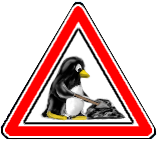
\includegraphics[width=0.1\linewidth]{./Figures/tux-development}
}

\author{Jorge Alejandro Tarango Yong}
\DeclareCaptionFormat{cont}{#1 (cont.)#2#3\par}
\begin{document}
\maketitle
\pagestyle{empty}
\begin{center}

\includegraphics[width=0.2\linewidth]{./Figures/logoUNAM}

\large
\textbf{UNIVERSIDAD NACIONAL AUTÓNOMA DE MÉXICO}

\rule{\linewidth}{0.1pt}

\rule[3mm]{0.7\linewidth}{1pt}


INSTITUTO DE RADIOASTRONOMÍA Y ASTROFÍSICA
\\[3\baselineskip]
``Estudio de la Interacción de Flujos Múltiples de Fuentes Astrofísicas, Aplicada
a los Proplyds Clásicos de la Nebulosa de Orión''
\\[2\baselineskip]

T E S I S
\\[2\baselineskip]
PARA OBTENER EL GRADO ACADÉMICO DE

DOCTOR EN CIENCIAS (ASTRONOMÍA)
\\[2\baselineskip]

P R E S E N T A
\\[2\baselineskip]
JORGE ALEJANDRO TARANGO YONG

Director de Tesis: Dr. William J. Henney
\\[2\baselineskip]
\normalsize
\end{center}
\begin{flushright}
Morelia, Michoacán

2017

\end{flushright}

\tableofcontents
\newpage
\section*{Agradecimientos}

% Esta tesis se realizó para obtener el título de doctorado en ciencias (Astronomía). Deseo aprovechar esta sección para hacer agradecimientos a personas y/o instituciones que me ayudaron para que pueda completar este trabajo de manera exitosa.
Primero que nada debo agradecer al Instituto de Radioastronomía y Astrofísica por haberme dado el priviligio de formar parte del Posgrado en Astrofísica para obtener el título de Doctor en Astrofísica. La dedicación, la disciplina y el pensamiento crítico son algunas de las habilidades que adquirí durante la estancia de esta magnífica institución.

En segunda agradezco al Consejo Nacional de Ciencia y Tecnología (CONACyT) por haberme asignado una beca nivel Nacional, del año 2013 al 2017, mi número CVU es 378230.

También quiero agredecer a mi asesor Will por su paciencia, sus buenos consejos y por todo lo que pude aprender de él tanto en la maestría como en el doctorado, y por la oportunidad que me dio de presentar mi trabajo en aquel congreso en Grecia.

A Karin por su amistad y por la ayuda que nos proporcionó durante todo en posgrado. A Rafa también por su amistad y por toda la trayectoria en materia de divulgación que tuve durante mi estancia en el instituto.

Mis padres también tienen una parte especial de mí: ellos me ayudaron cuando terminó el contrato de mi beca CONACyT: de no ser por su ayuda, esta tesis hubiera tomado aún más tiempo terminarla. También sus consejos y su cariño han sido fundamentales para poder llegar a ser quien soy el día de hoy.

Por último y no menos importante, a mi familia: mi amada esposa Betty y mi hija Carmen. Por ellas es por quienes tengo fuerzas todas las mañanas de levantarme y seguir adelante, aunque el resto de mi cuerpo y mi mente me digan lo contrario. A veces parece que no es así, pero nunca estaré arrepentido de que estén a mi lado, y nunca me rendiré para que podamos salir adelante, no importa el tiempo que tome.
\newpage
\section*{Resumen}
  Abstract en español

\newpage
\section*{Abstract}
  Abstract written in english

\newpage
\section*{\centering Prefacio}

Los choques de proa se producen cuando un flujo de gas con simetría esférica se mueve a velocidades supersónicas e interactúa con el medio que lo rodea. Aparecen en diferentes escenarios astrofísicos, como mencionaremos más adelante.

En trabajos anteriores se intentó obtener información relevante acerca de las propiedades de choques de proa dentro de la Nebulosa de Orión producidos por proplyds basándose en mediciones de su forma aparente \citep{Robberto:2005}, sin embargo, las mediciones de algunos de estos choques no concordaban con el modelo teórico utilizado para obtener dicha información. La motivación inicial de este trabajo consistía en extender el modelo de aproximación de capa delgada para la interacción de dos vientos \citep{Canto:1996} para incluir el escenario donde el viento interior deja de ser isotrópico, esperando que las mediciones de la forma del choque producido por esta clase de vientos ajuste mejor a la forma de los choques de proa restantes en la Nebulosa de Orión.

Esta tesis está estructurada de la siguiente manera: en el capítulo \ref{chap:ONC} mencionamos algunas características generales de la Nebulosa de Orión, la región \Ion{H}{II} por excelencia para estudiar el escenario de la formación estelar y donde se han encontrado una gran variedad de objetos y fenómenos astrofísicos de gran interés, así como el modelo aceptado actualmente de la formación de los proplyds, que son los que producen los choques de proa observados en las Nebulosa de Orión, y muy probablemente en otras regiones \Ion{H}{II}. En el capítulo \ref{chap:bow-shocks} se explican diferentes escenarios donde se pueden formar choques de proa. En el capítulo \ref{chap:Modelo-generico} se explican conceptos fundamentales que nos serán de gran utilidad para entender los modelos de interacción de vientos de los que obtendermos la forma de los choques de proa, tales como los ``radios característicos'', que son los parámetros medibles con los que determinaremos la forma de los choques de proa. También explicaremos como para un choque geométricamente delgado y ópticamente delgado su orientación respecto al plano del cielo influye en la forma que observamos, y lo ejemplificamos con las formas más simples (aunque no necesariamente plausibles físicamente): las cuádricas de revolución. El capítulo \ref{chap:hipersonica} explica a detalle el modelo de capa delgada de \citet{Canto:1996} en el que nos basamos para modelar la forma de los choques de proa, y explicamos la extensión a este modelo que realizamos. Asimismo mostramos cómo sería su forma aparente si su eje de simetría no estuviera en el plano del cielo. En el capítulo \ref{chap:proplyds} aplicamos los resultados de los capítulos anteriores a los choques de proa formados por los proplyds de la Nebulosa de Orión. Por último, en el capítulo \ref{chap:conclusions} enumeramos las conclusiones finales de este trabajo.

Esta tesis también cuenta con apéndices donde explicamos a detalle conceptos importantes para esta tesis: los apéndices \ref{app:HII}-\ref{app:shocks} explican el modelo actual de las regiones \Ion{H}{II} y la física detrás de los choques y Frentes de Ionización, que nos ayudará a entender cómo se forma el viento fotoevaporado e ionizado de un proplyd. El apéndice \ref{app:math-curvature-radius} contiene el procedimento matemático con el que se define y se calcula el Radio de Curvatura (uno de nuestros radios característicos) para una curva genérica, siempre y cuando sea continua y derivable. El apéndice \ref{app:derivation-radii} explicamos de manera detallada cómo se obtienen las ecuaciones para calcular los radios característicos en el modelo de capa delgada. Por último, en el apéndice \ref{app:article} mostrmos el artículo en que se basa gran parte de esta tesis (parte del capítulo \ref{chap:bow-shocks} y los capítulos \ref{chap:Modelo-generico} - \ref{chap:hipersonica}), actualmente publicado (el capítulo \ref{chap:proplyds} se basa en un artículo que aún no está terminado y probablemente los resultados presentados aquí serán incluídos).

\newpage

  

\pagestyle{fancy}
\fancyhf{}
\fancyhead[LE]{\footnotesize \thepage \quad\leftmark}
\fancyhead[RO]{\footnotesize \rightmark \quad\thepage}
\chapter[La Nebulosa de Orión]{La Nebulosa de Orión: La Fotoevaporación de Discos Protoplanetarios como una Forma de Feedback Estelar}
\thispagestyle{empty}
\label{chap:ONC}
\section{Características Generales}
\begin{figure*}
  \centering
  \begin{tabular}{cc}
    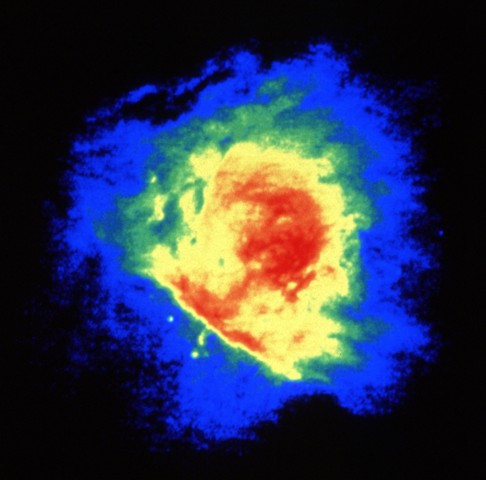
\includegraphics[width=0.5\linewidth]{./Figures/OrionVR13A} & 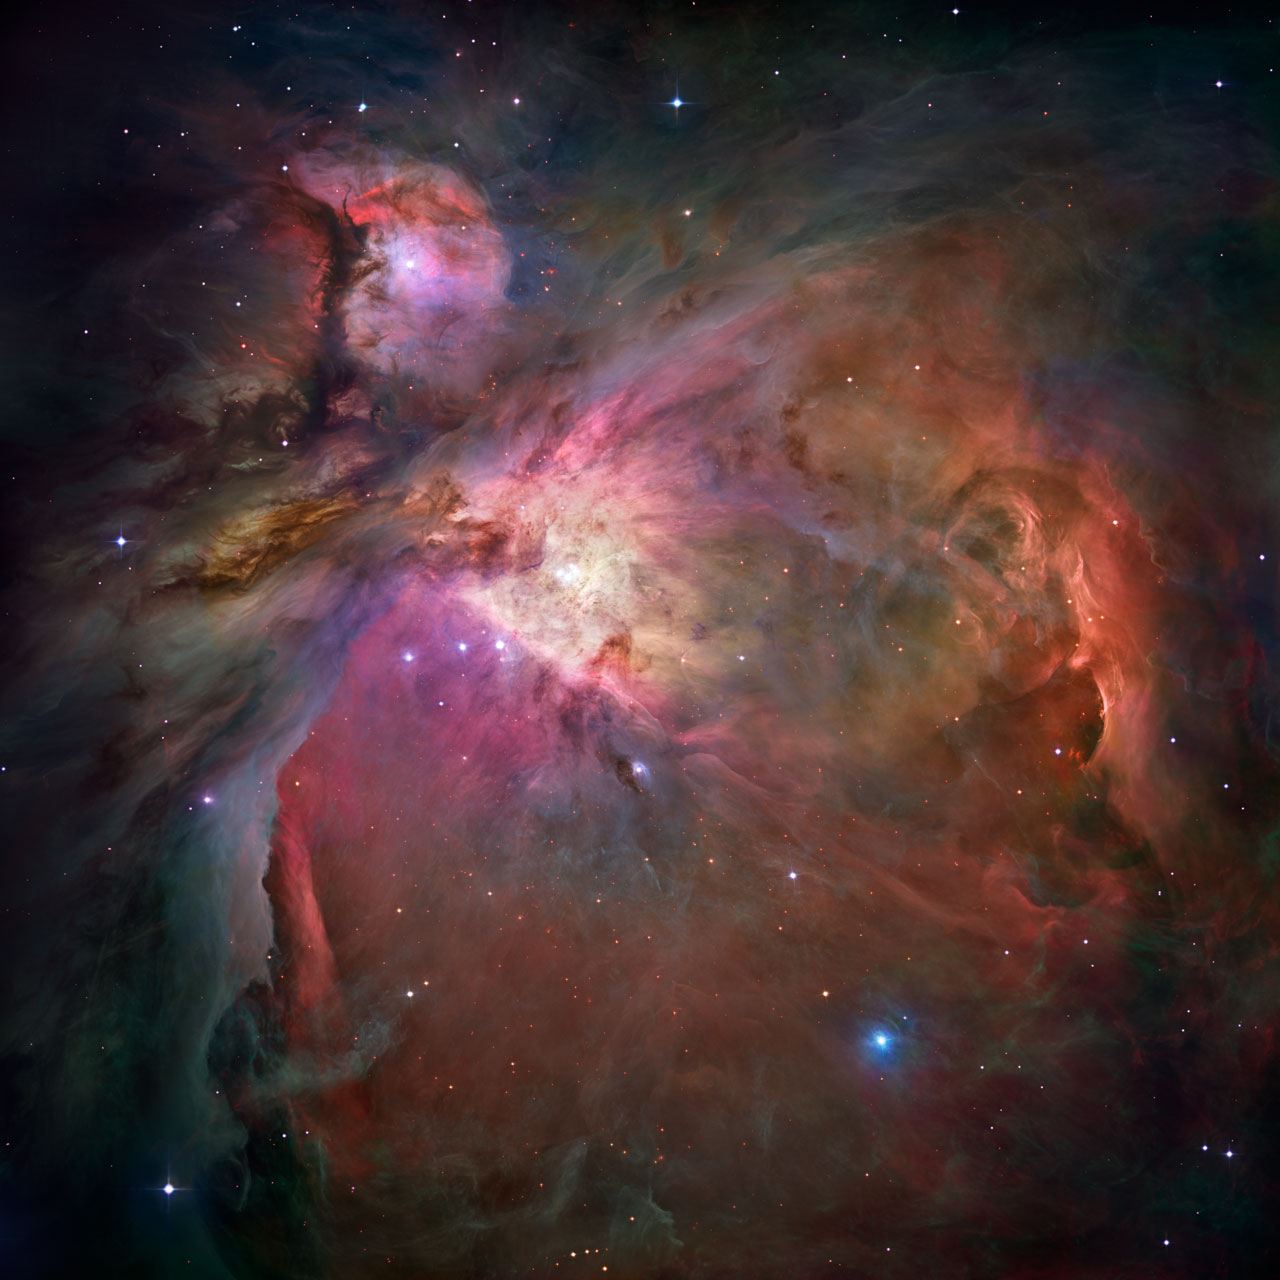
\includegraphics[width=0.5\linewidth]{./Figures/ONC-HST}
  \end{tabular}
  \caption{Izquierda:La Nebulosa de Orión observada por el VLA en la banda L ($\lambda = \SI{20}{cm}$, $\nu = \SI{1.4}{GHz}$, \citet{Yusef:1990}). Derecha: la nebulosa de Orion tomada con el Telescopio Espacial Hubble (hubblesite.org).}
\end{figure*}

El cúmulo de las Nebulosa de Orión (ONC por sus siglas en inglés), ubicada a $\sim \SI{414}{pc}$ \citep{Menten:2007}, es probablemente la región \Ion{H}{II} mejor estudiada del cielo (ver apéndice \ref{app:HII}). Forma parte de la nube molecular gigante de Orión, de donde se distinguen dos sub-unidades, llamadas Orión A y Orión B. ONC forma parte de Orión A. El cúmulo de estrellas masivas que se formó y que es responsable de la región \Ion{H}{II} se conoce como asociación OB Ori Id, cuyos miembros más prominentes son un grupo de cuatro estrellas conocidas como el ``Trapecio''. La más masiva de éstas es \thC{}, de clasificación espectral O6 aproximadamente (ver tabla \ref{tab:ionizing-radiation}), tiene una luminosidad de \SI{4e5}{L_\odot} y una temperatura de \SI{4e4}{K}. Cuando la región \Ion{H}{II} se encuentra embebida en el gas molecular, no puede ser visible en el rango óptico del espectro. En el caso de ONC, que se ubica cerca del borde de la nube molecular Orion A, el gas ionizado caliente, que posee una presión mayor que el gas molecular frío, se escapa hacia el gas adyacente a la nube molecular en forma de ``flujo de champaña'' (figura \ref{fig:champagne}), y de esta manera el gas ionizado puede ser visible por medio de diferentes líneas espectrales, tanto de hidrógeno como de otros elementos. 

\begin{figure}
  \centering
  \begin{tabular}{lr}
    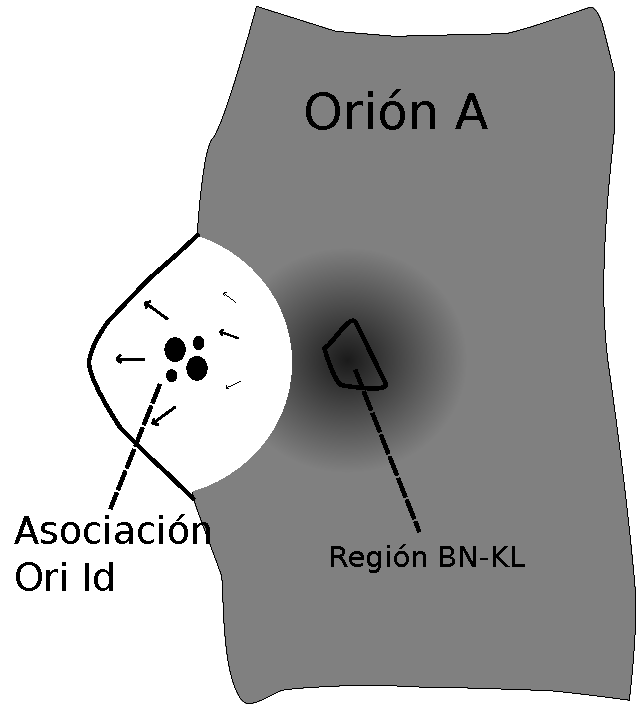
\includegraphics[width=0.4\linewidth]{./Figures/champagne} &
    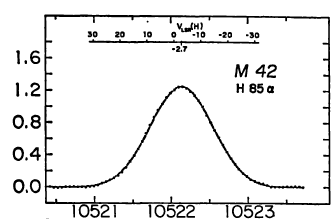
\includegraphics[width=0.5\linewidth]{./Figures/H85-alpha}
    \end{tabular}
  \caption{Izquierda: Representación esquemática de la Asociación Ori Id y su ubicación dentro de la nube molecular gigante Orión A. La región BN-KL es una región de formación estelar muy activa donde se observan entre otras cosas, máseres de agua y SiO y flujos moleculares \citep{Stahler:2004}. Derecha: Línea espectral \Ion{H85}{\alpha} de hidrógeno de ONC. El eje horizontal corresponde a la frecuencia en MHz, mientras que el eje verical representa la temperatura de antena. El espectro muestra un corrimiento al azul que muesta que el gas se acerca a una velocidad de $\sim \SI{3}{km.s^{-1}}$ \citep{Stahler:2004, Churchwell:1970}}
  \label{fig:champagne}
\end{figure}

\section{Proplyds}
\subsection{Descubrimiento}
Observaciones en óptico de la región del Trapecio en filtros de banda angosta de diferentes líneas de emisión tales como \Ion{H}{\alpha}, \Ion{H}{\beta}, [\Ion{O}{III}], [\Ion{N}{II}], [\Ion{S}{II}] y continuo, revelaron la existencia de objetos puntuales visibles notablemente en líneas de alta ionización (\Ion{H}{\alpha}, \Ion{H}{\beta} y [\Ion{O}{III}]) que fueron inicialmente denominados como ``condensaciones nebulares'' \citep{Laques:1979}. Hasta ese momento no se sabía con certeza si esas ``condensaciones nebulares'' eran en realidad condensaciones nebulares (regiones donde la densidad de la nebulosa es inusualmente alta por alguna razón o bien esferas de gas molecular cuya envolvente fue ionizada y que la radiación de la estrella central la está ``erosionando'') o si se trataba de protoestrellas de baja masa cuyo disco protoplanetario estaba siendo fotoevaporado por la estrella central \citep{churchwell:1987}. No fue sino hasta que se contó con observaciones de alta resolución con el Telescopio Espacial Hubble (HST) que se se pudo determinar la verdadera naturaleza de estos objetos \citep{ODell:1993} y la razón por la que se les denominó ``proplyds'' (PROtoPLanetarY DiskS). A su vez se encontraron por primera vez arcos delgados y otras estructuras de gran interés.

\subsection{¿Qué es un proplyd? Breve introducción \citep{Johnstone:1998}}
\label{sec:prop-Johnstone}

Las imágenes del HST de la Nebulosa de Orión mostraron imágenes de discos alrededor de estrellas jóvenes de baja masa. Algunos se ven como siluetas oscuras que contrastan con la nebulosa, y otros casos son visibles en líneas de emisión de líneas de alta ionización. Un proplyd típico tiene forma cometaria, con una cabeza brillante que apunta hacia la fuente de radiación ionizante, y una cola que se extiende en dirección contraria a ésta. La explicación a esta forma es que se trata de estrellas T-Tauri que quedaron embebidas por la región \Ion{H}{II} en expansión y el disco protoplanetario está siendo fotoevaporado por la radiación ionizante de una estrella masiva (\thC{} en caso de la Nebulosa de Orión), la cabeza es un frente de ionización cuyo radio escala como $R_{\mathrm{IF}} \propto D^{2/3}$, donde $D$ es la distancia a la estrella masiva. La forma de la cola se debe a radiación ionizante difusa, producto de dispersión por polvo y por recombinaciones (Figura \ref{fig:prop-shape}). \citet{churchwell:1987} ya había notado que la tasa de pérdida de masa observada en el gas ionizado implicaba que la fuente de este gas debía oscurecer a la protoestrella huésped, a menos que proviniera de un disco circunestelar. De la emisión de radio observada, se estima que la densidad electrónica máxima en el IF es de $n_e \sim \SI{e6}{cm^{-3}}$ y la tasa de pérdida de masa es de $\dot{M} \sim \SI{e-7}{M_\odot.yr^{-1}}$.

\begin{figure}
  \centering
  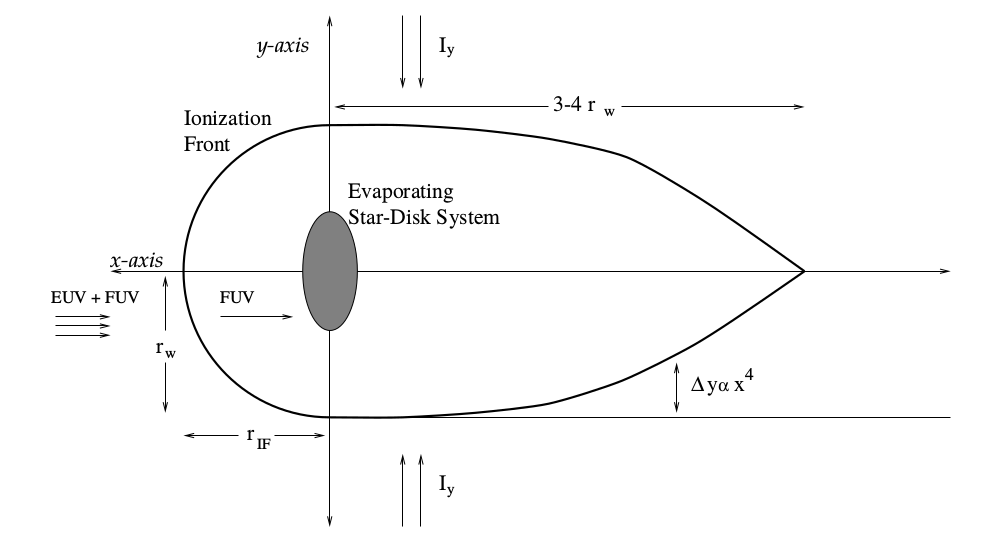
\includegraphics[width=0.8\linewidth]{./Figures/Johnstone-shape}
  \caption{Representación esquemática de la formación de un frente de ionización hemisférico y de una cola de gas ionizado detrás del disco en proceso de fotoevaporación. $r_{\mathrm{IF}}$ y $r_w$ representan el radio del frente de ionización en las direcciones de los ejes $x$ e $y$, respectivamente. $I_y$ representa el campo de radiación difusa. Por detrás del disco, la radiación difusa calienta el gas del disco provocando otro flujo fotoevaporado. $\Delta y$ es la diferencia entre la forma actual del frente de ionización por detrás del disco y una forma cilíndrica. La forma de la colase explica como que el flujo de radiación $I_y$ es capaz de penetrar más cerca del eje $x$ conforme uno se aleja del disco, donde el flujo fotoevaporado es menos denso.}
    \label{fig:prop-shape}
\end{figure}


\subsection{Mecanismos de fotoevaporación \citep{Johnstone:1998}}
\label{sec:photoevaporation}

El principal mecanismo de fotoevaporación es el campo de radiación de la estrella central, en la parte ultravioleta del espectro electromagnético. Según la masa de la estrella central, podemos tener dos clases de flujo radiativo: Dominado por el ultravioleta lejano (FUV, $h\nu < \SI{13.6}{eV}$) o dominado por el ultravioleta extremo (EUV, $h\nu \geq \SI{13.6}{eV}$). En general, el FUV se encarga de disociar moléculas y de calentar el gas de la región de fotodisociación (PDR) hasta temperaturas de \SI{100}{} - \SI{1000}{K}, mientras que el EUV puede ionizar el gas y elevar su temperatura hasta \SI{e4}{K}. El EUV no puede atravesar el frente de ionización (IF) pero el FUV sí.

En el caso de que el flujo sea dominado por el EUV, la presión térmica del flujo fotoevaporado es determinada por la fotoionización, la PDR producida por el FUV es delgada. El gas calentado por el FUV se mueve de manera subsónica hasta llegar al IF y la tasa de pérdida de masa depende de la tasa de ionización inducida por el EUV.

Si el flujo está dominado por el FUV, la presión térmica depende del calentamiento por el FUV. El gas tibio se expande como un viento que empuja el IF lejos del disco. La tasa de pérdida de masa la determina la temperatura de la PDR, el flujo FUV y la opacidad del polvo a las longitudes de onda del FUV. Inicialmente la forma del disco impone una geometría cilíndrica en el flujo fotoevaporado, pero eventualmente los gradientes de presión tornan esta geometría en esférica.

Las ecuaciones de continuidad de la masa y el momento restringen la velocidad del flujo neutro antes de alcanzar el IF. Mas allá de éste, la presión del gas hace que éste se expanda a velocidades del orden de una a dos veces la velocidad del sonido, que es de $c_{\mathrm{I}} \sim \SI{3}{km.s^{-1}}$ para el gas neutro, y de $c_{\mathrm{II}} \sim \SI{10}{km.s^{-1}}$ para el gas ionizado. Para el gas neutro dentro del IF hay dos posibles soluciones: si el gas neutro es supersónico entonces el IF será de baja densidad (Tipo R) con bajo contraste de densidad entre gas neutro y gas ionizado. O si el gas neutro es subsónico se formará un IF tipo D con un gran contraste de densidad entre el gas neutro y el gas ionizado. Sin embargo, sin importar qué tipo de radiación domina la fotoevaporación, el gas neutro permanece a velocidades subsónicas al llegar al IF, por lo que dicho frente será tipo D. En el caso de un flujo dominado por el EUV, el gas neutro permanece a velocidad subsónica, su velocidad decae como $v_I \propto r^{-2}$ y llega a \SI{0.5}{km.s^{-1}} al llegar al frente de ionización. Cundo el flujo es dominado por el FUV, el gas neutro se acelera hasta llegar a velocidades supersónicas, luego atraviesa un choque isotérmico que lo desacelera y llega al frente de ionizacion a \SI{0.5}{km.s^{-1}}.

\begin{figure}
  \centering
    \begin{tabular}{cc}
      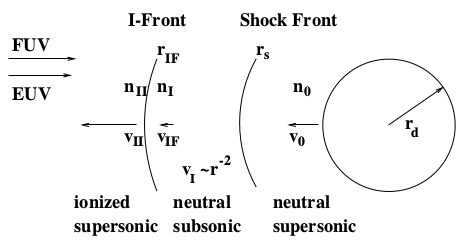
\includegraphics[width=0.5\linewidth]{./Figures/Johnstone-2} &
      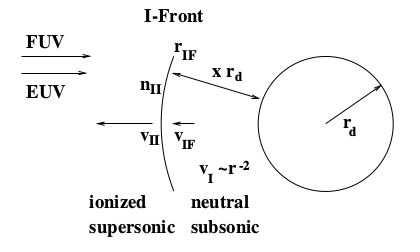
\includegraphics[width=0.5\linewidth]{./Figures/Johnstone-3}
    \end{tabular}
    \label{fig:EUV-FUV-IF}
    \caption{Representación esquemática de las regiones del flujo fotoevaporado de un proplyd. Izquierda: Cuando el flujo es dominado por el FUV. Derecha: Flujo dominado por EUV \citep{Johnstone:1998}}
  \end{figure}
  
  
Sin importar el tipo de mecanismo de fotoevaporación dominante, el flujo fotoevaporado existe solo si la presión térmica supera a la gravedad de la protoestrella. Entonces, el flujo fotoevaporado solo existe a partir de un radio crítico $r_g$, donde este radio se estima a partir del balance entre la energía necesaria para escapar de una órbita kepleriana y la energía térmica:
\begin{align}
  r_g = \frac{GM_*}{c^2}
\end{align}
Donde $M_*$ es la masa de la protoestrella y $c$ es la velocidad del sonido del gas. Para las protoestrellas típicas del Trapecio la masa típica es de
$M_* = \SI{0.2}{M_\odot}$. Utilizando las velocidades del sonido para el gas neutro e ionizado, encontramos que el radio gravitacional para un flujo dominado por el EUV es de $r_{\mathrm{gII}} \sim \SI{2}{AU}$ y para un flujo dominado por el FUV es de $r_{\mathrm{gI}} \sim \SI{20}{AU}$.

\chapter[Choques de Proa]{Choques de Proa en el Medio Interestelar}
\label{chap:bow-shocks}
\thispagestyle{empty}

En general, un choque de proa se forma cuando un fluido interactua con un objeto moviéndose a velocidades supersónicas. A continuación enumeramos algunos ejemplos astrofísicos que se pueden encontrar en el Medio Interestelar:

\begin{itemize}
\item Superficies de trabajo de jets
\item Interacción de magnetósfera con el viento solar
\item Choques de proa estelares
  \begin{itemize}
  \item Estrellas AGB
  \item Estrellas O
  \item \textbf{Proplyds}
  \item Estrellas T Tauri
  \item Estrellas de Neutrones
  \end{itemize}
\end{itemize}

La morfología general de un choque de proa se ilustra en la figura \ref{fig:terminology}. La región donde la distancia entre el choque y la estrella (en el caso de un choque de proa \textit{estelar}) es la mínima, se denomina cabeza o \textit{ápex}, mientras que las regiones más alejadas son denominadas las \textit{alas}. En el caso ideal los choques de proa son cilíndricamente simétricos.

\begin{figure}
  \centering
  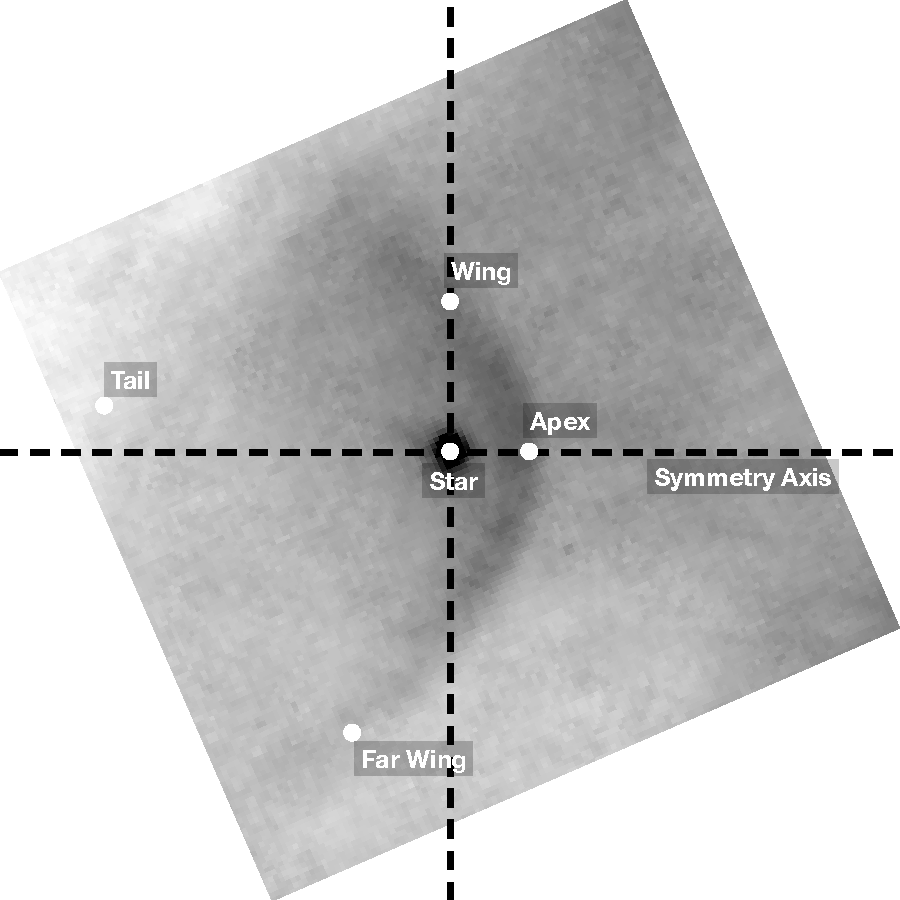
\includegraphics[width=0.5\linewidth]{./Figures/bow-terminology}
  \caption{Terminología de un choque de Proa \textit{estelar}.}
  \label{fig:terminology}
\end{figure}

\section{Proplyds}
Observaciones en mediano infrarrojo y en líneas de emisión de \Ion{H}{\alpha} y [\Ion{O}{III}] \citep{Robberto:2005, Bally:1998, Bally:2000} muestran de manera clara la presencia de arcos que rodean varios proplyds y otros objetos en la ONC cerca y lejos e la región del Trapecio. \citet{Hayward:1994} abre por primera vez la discusión acerca de la naturaleza de estos arcos (enfocándose en la región del Trapecio), sugiriendo que la presión de radiación y el viento estelar de \thC{} interactúan con el flujo de gas proveniente de cada proplyd individual.

\begin{figure}
  \centering
  \begin{tabular}{lr}    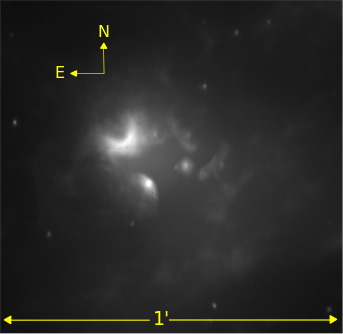
\includegraphics[width=0.5\linewidth]{./Figures/Orion_Robberto}&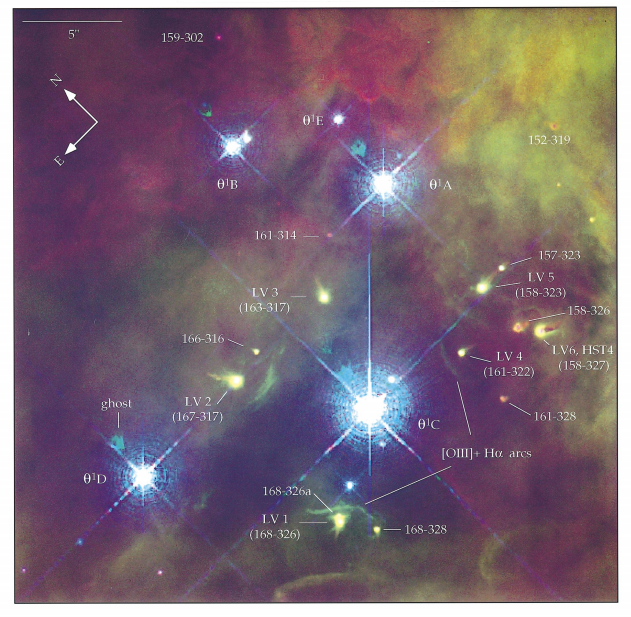
\includegraphics[width=0.5\linewidth]{./Figures/bally-trapezium}
  \end{tabular}
  \caption{Izquierda: La región del trapecio en \SI{10}{\mu m}. \thC{} es la fuente débil al centro de la imagen. Dentro de este campo además se encuentran los proplyds LV1-LV5 con sus respectivos arcos. Al noreste se encuentra una fuente extensa llamada la Nebulosa Ney Allen (NA). El norte es encuentra hacia arriba y el este a la izquierda. El tamaño del campo es de aproximadamente $1' \times 1'$ \citep{Robberto:2005}. Derecha: La región del trapecio en mosaico de colores con imágenes de la Cámara Planetaria de Campo Ancho 2 (WPC2) del ciclo 4 del Telescopio Espacial Hubble (HST). El color rojo corresponde al [\Ion{N}{II}], el verde al \Ion{H}{\alpha} y el azul es [\Ion{O}{III}] \citep{Bally:1998}.}
\end{figure}

Asimismo, en \citet{Robberto:2005} se hicieron mediciones de la forma de estos arcos, utlizando el radio aparente en el ápex $R_0/D$ y el radio perpendicular a éste $R_{90}/D$ (la alatud en este trabajo, excepto que normalizada con la distancia a \thC{} $D$, ver \S \ref{sec:char-rad}) para los proplyds LV1-LV5 y la nebulosa Ney-Allen, y los compararon con el modelo de capa delgada \citep{Canto:1996} (figura \ref{fig:Robberto}). Encontraron que aunque los proplyds LV1, LV4 y posiblemente LV5 ajustan a dicho modelo, pero el resto se aleja mucho de las curvas teóricas. Ésto no se puede atribuir atribuir a las limitaciones de la aproximación algebraica hecha por \citet{Canto:1996}, debido a que aun con todas las simplificaciones que conlleva, ajusta bien con modelos hidrodinámicos más complejos (\citet{Garcia-Arredondo:2001}, figura \ref{fig:GA-simulation}). Este trabajo es en parte la inspiración para esta tesis, ya que para explicar la discrepancia en la figura \ref{fig:Robberto} con los proplyds restantes nos llevó a extender el modelo de \citet{Canto:1996} al caso donde el viento interior no es isotrópico. En la figura \ref{fig:generic-bowshock} se explica el modelo general para explicar éstos choques de proa: el flujo fotoevaporado de un proplyd, ya sea isotrópico o anisotrópico, interactúa con el viento estelar de \thC{}, formando dos choques separados por una discontinuidad de contacto. El Frente de Ionización del proplyd es tipo D (ver \S \ref{sec:photoevaporation}), por lo que la velocidad del flujo fotoevaporado es cercano a la velocidad del Sonido y se acelera máximo hasta $M\sim 3$, y su densidad electrónica es de $n_e\sim \SI{e6}{cm^{-3}}$ (ver \S \ref{sec:prop-Johnstone}). Por otro lado, el viento de \thC{} ha alcanzdo su velocidad terminal, que es de $M > 100$ con una tasa de pérdida de masa de $\dot{M} \simeq \SI{4e-7}{M_\odot.yr^{-1}}$ \citep{Gagne:2005}. Bajo estas condiciones, el choque exterior es poco denso y extenso y el choque interior es más denso y angosto. Por tanto, el enfriamiento en el choque interior es más eficiente y consideramos que este choque es radiativo mientras que el choque exterior no.

\begin{figure}
  \centering
  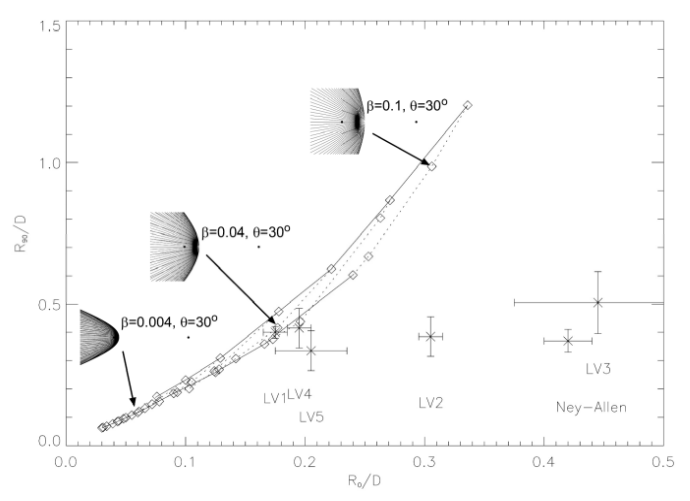
\includegraphics[width=0.7\linewidth]{./Figures/robberto}
  \caption{Comparación de los Radio Característicos aparentes $R'_{90}/D$ y $R_0/D$ para los proplyds LV1-LV5 y para la Nebulosa Ney-Allen mostrados con puntos y sus respectivas incertidumbres, y los diamantes abiertos se muestran soluciones al modelo de capa delgada de \citep{Canto:1996} para $\beta=[0.001, 0.002, 0.004, 0.01, 0.02, 0.1]$ y para intervalos de inclinaciones de $15^\circ$ entre $0^\circ$ y la inclinación máxima (ver \S \ref{sec:fundamental-parameters}, \ref{sec:projection}).}
  \label{fig:Robberto}
\end{figure}

\begin{figure}
  \centering
  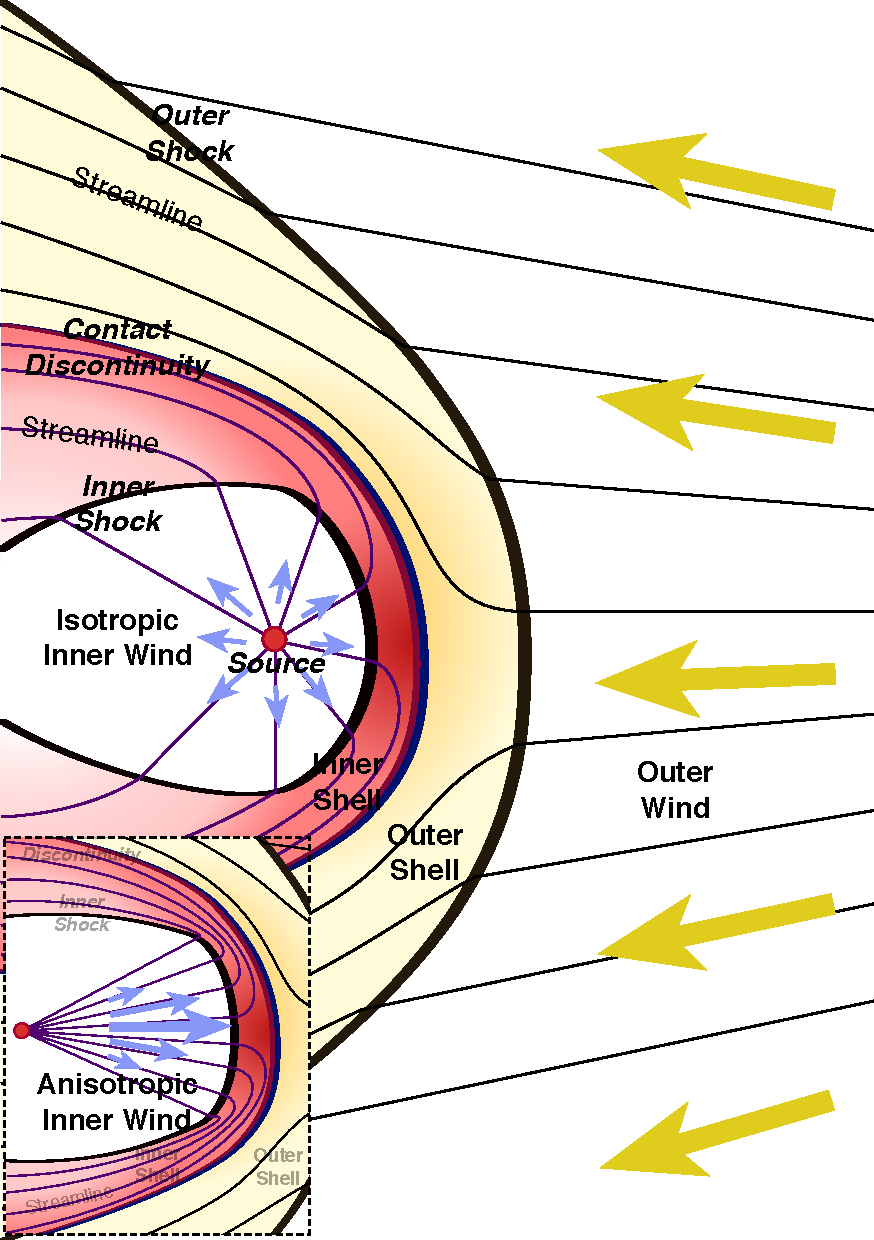
\includegraphics[width=0.7\linewidth]{./Figures/generic-bowshock}
  \caption{Esquema del choque de proa de un proplyd: el viento rápido proveniente de una estrella masiva interactúa con el flujo fotoevaporado de un proplyd que puede ser isotrópico o anisotrópico. Se forman dos choques separados por una discontinuidad de contacto, y dependiendo de la velocidad y densidad de los vientos, dichos choques pueden ser radiativo o no. En el caso de los proplyds más cercanos al trapecio, solo el choque interno es radiativo.}
  \label{fig:generic-bowshock}
\end{figure}


\begin{figure}
  \centering
  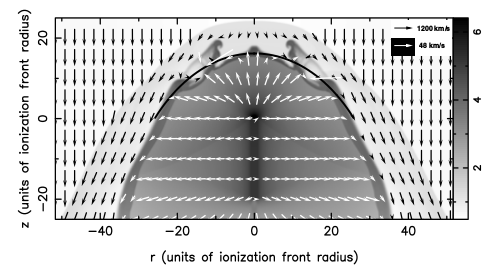
\includegraphics[width=0.7\linewidth]{./Figures/GA-simulation}
  \caption{Resultado de una simulación hidrodinámica de la interacción de un flujo fotoevaporado de un proplyd con un viento estelar. Las flechas indican la velocidad de los flujos (negro para el viento estelar y blanco para el flujo fotoevaporado del proplyd) y la escala gris representa el logaritmo de la densidad. Los ejes están en coordenadas cilíndricas $(r, z)$ en unidades del radio del IF. El arco negro representa la solución analítica de la posición de la discontinuidad de contacto de un choque ancantoide con $k=1/2$ y $\beta=0.002$ \citep{Garcia-Arredondo:2001}}
  \label{fig:simulation}
\end{figure}

\section[Objetos LL]{Choques de Proa ``In Situ'': Objetos LL'}

El arquetipo de esta clase de objetos es LL\,Ori (LL1 de aquí en adelante), son llamados también choques ``in situ'' \citep{Kobulnicky:2016}, donde el choque se da cuando viento de una estrella interactúa con un flujo tal como un flujo de champaña. Sin embargo, no es del todo claro el tipo de flujo interno proveniente de la estrell central (figura \ref{fig:LL-scheme}). \citet{Gutierrez-Soto:2015a} hizo un catálogo de objetos dentro de ONC en los que se observan choques de proa, algunos de ellos no habían sido identificados previamente, a la vez que se realizaron mediciones de $(R'_0, R'_c)$ de cada objeto (ver \S \ref{sec:fundamental-parameters}, \ref{sec:projection}). En las figuras \ref{fig:Luis-mosaic-1} y \ref{fig:Luis-mosaic-2} mostramos algunos ejemplos de este catálogo. A diferencia de los choques de proa más próximos a \thC{}, los objetos LL pueden presentar dos cáscaras. Si ese es el caso, los radios $(R'_0, R'_c)$ fueron medidos para ambas cáscaras, así como el grosor $H'$ que es la diferencia de $R'_0$ de ambas cáscaras y la orientación (figura \ref{fig:methodology-LL}).

\begin{figure}
  \centering
  \includegraphics[width=\linewidth]{./Figures/LL-outer-inner-extend-Luis}
  \caption{Posibiles escenarios para los flujos en interacción de los choques de proa en ONC. Izquierda: Un flujo de champaña transónico interactúa ya sea con el flujo fotoevaporado de un proplyd o con un viento estelar, este caso aplica para los arcos más alejados de \thC{}. Derecha: El viento estelar proveniente de una estrella tipo O interactúa con el flujo fotoevaporado de un proplyd. Aplica para los proplyds más cercanos a \thC{}.}
  \label{fig:LL-scheme}
\end{figure}

\begin{figure}
  \centering
  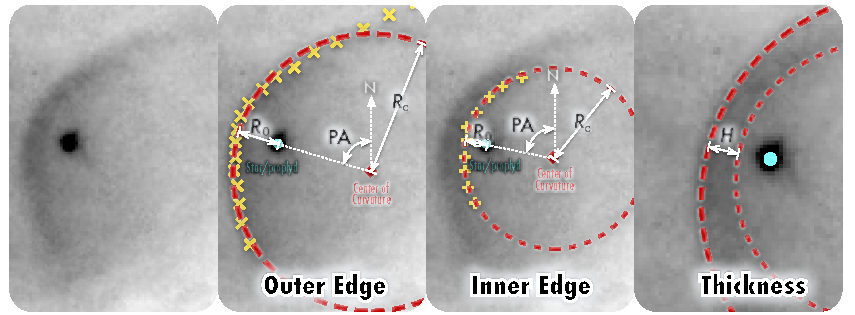
\includegraphics[width=0.7\linewidth]{./Figures/radius-methodology-Luis}
  \caption{Metodología para la medición de los radios característicos $(R'_0, R'_c)$. Para un arco dado, se traza la posición de las dos cáscaras utilizando marcas con el programa DS9 para imágenes astronómicas (las cruces en la figura). Posteriormente, con un ajuste de mínimos cuadrados se ajusta un círculo a las marcas de cada cáscara para obtener el radio de curvatura aparente $R'_c$ (línea roja rayada). $R'_0$ se obtiene como la distancia mínima entre la posición de la estrella y el ajuste circular y por último el grosor $H'$ se obtiene como la diferencia entre ambas mediciones de $R'_0$, suponiendo que estén disponibles.}
  \label{fig:methodology-LL}
\end{figure}

\begin{figure}
  \centering
  \begin{tabular}{cc}
    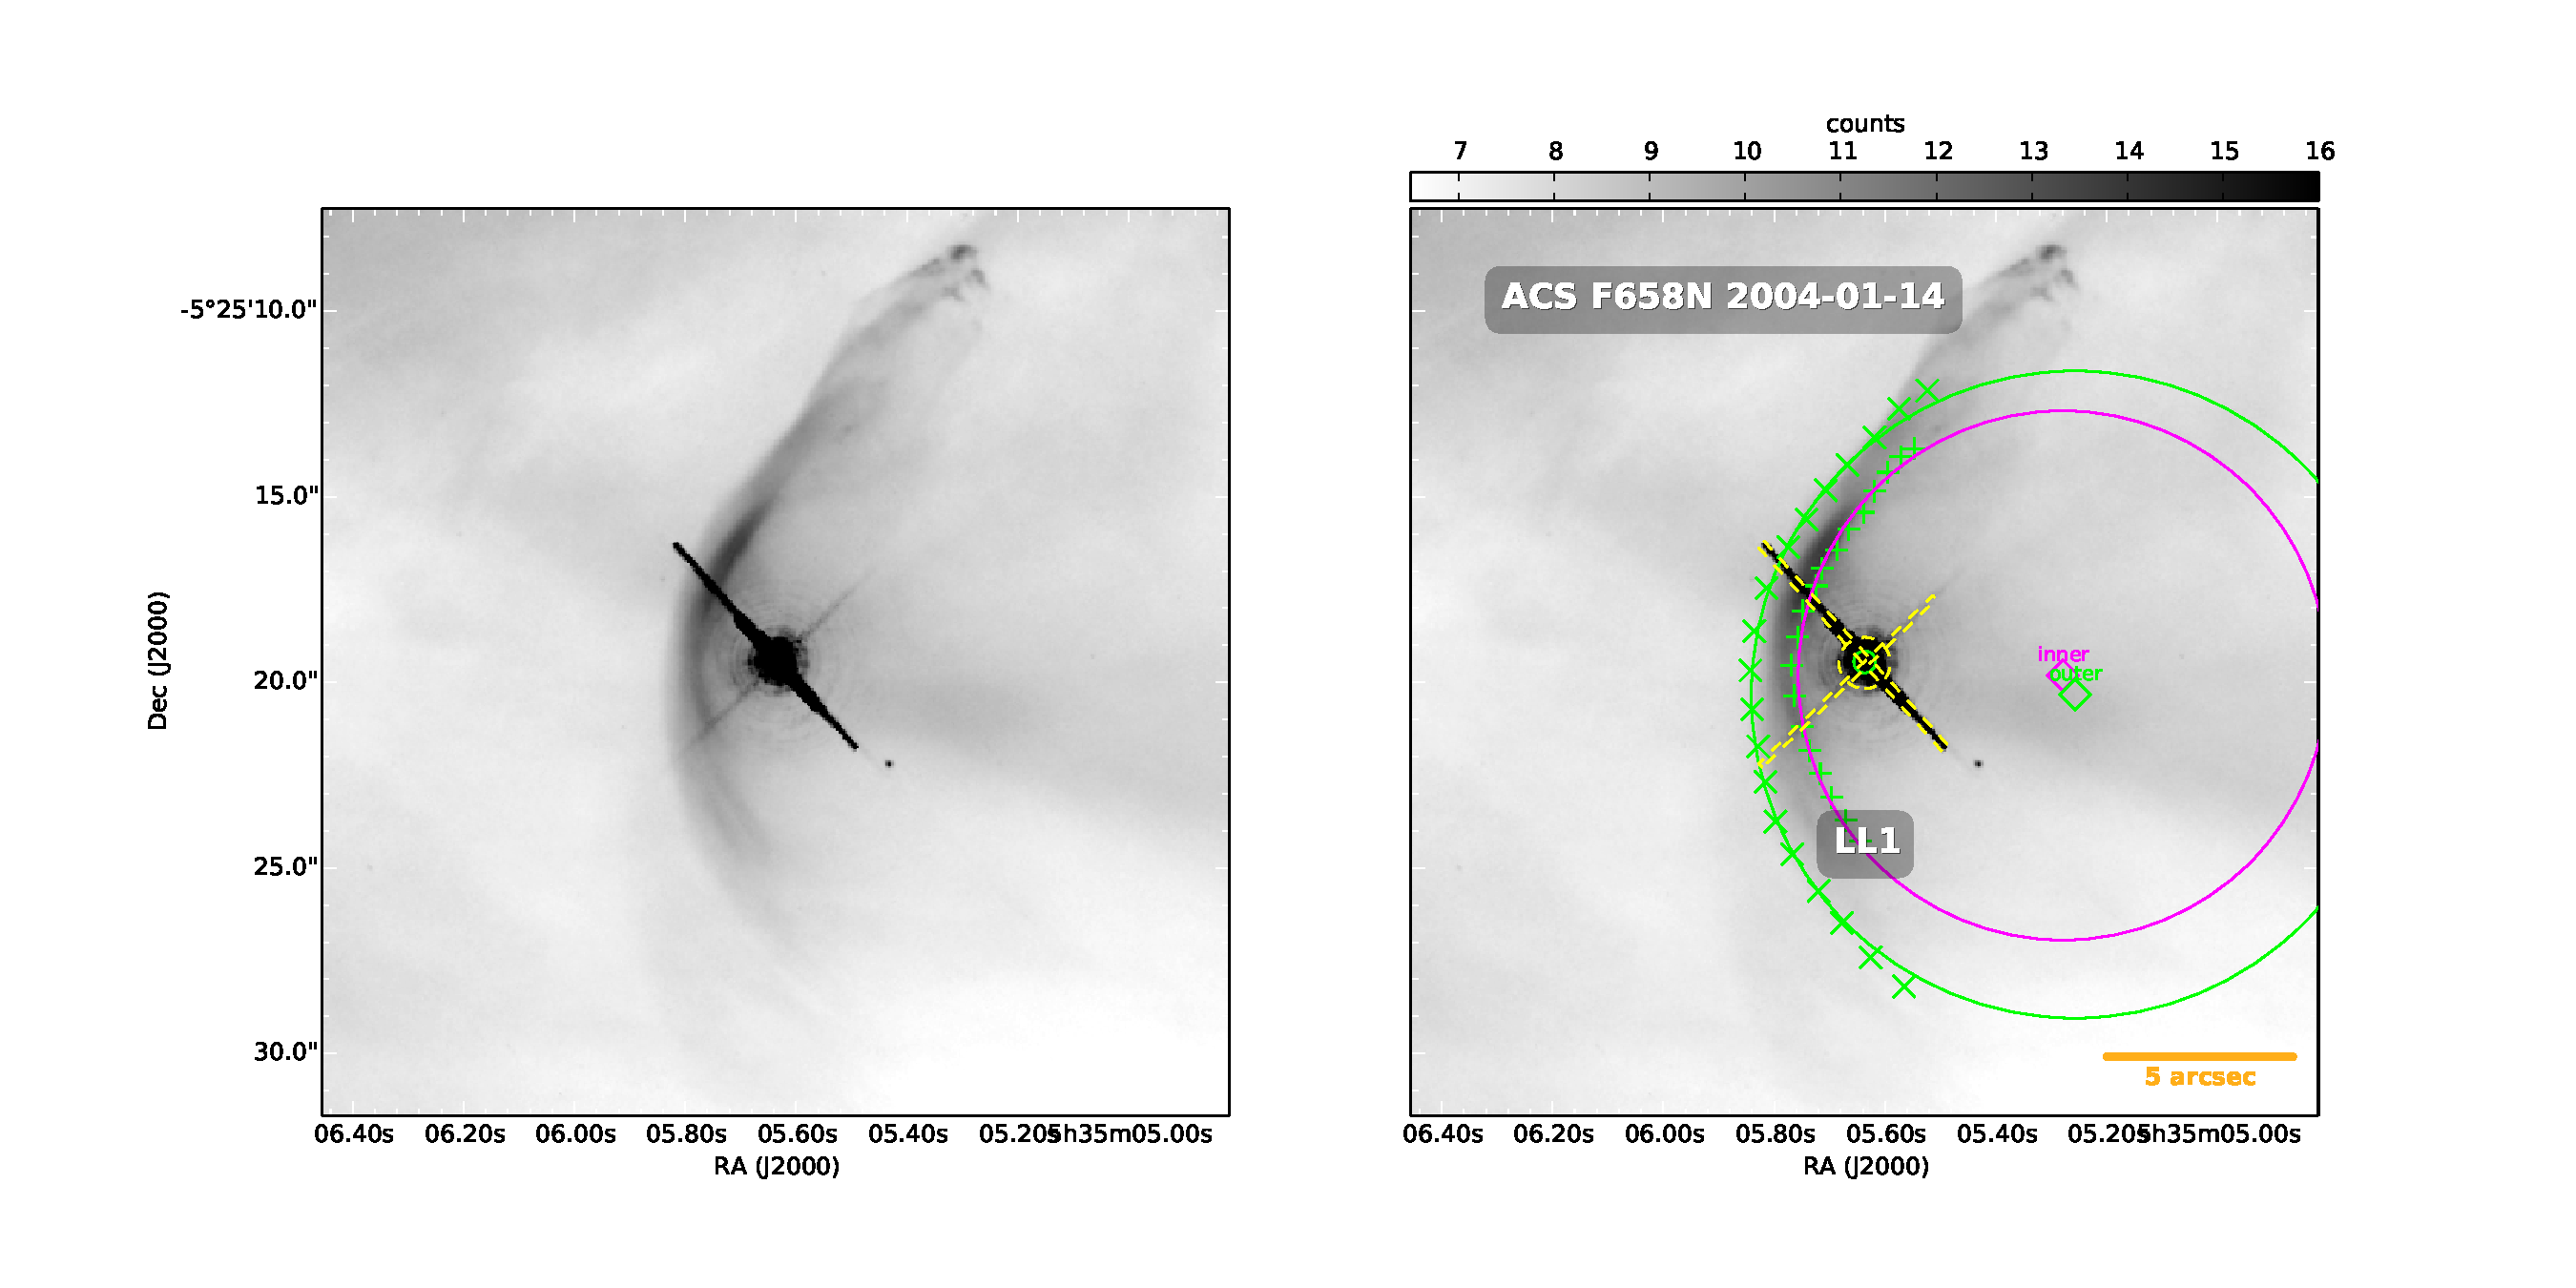
\includegraphics[width=0.5\linewidth]{./Figures/LL1-Bally_01-images} & 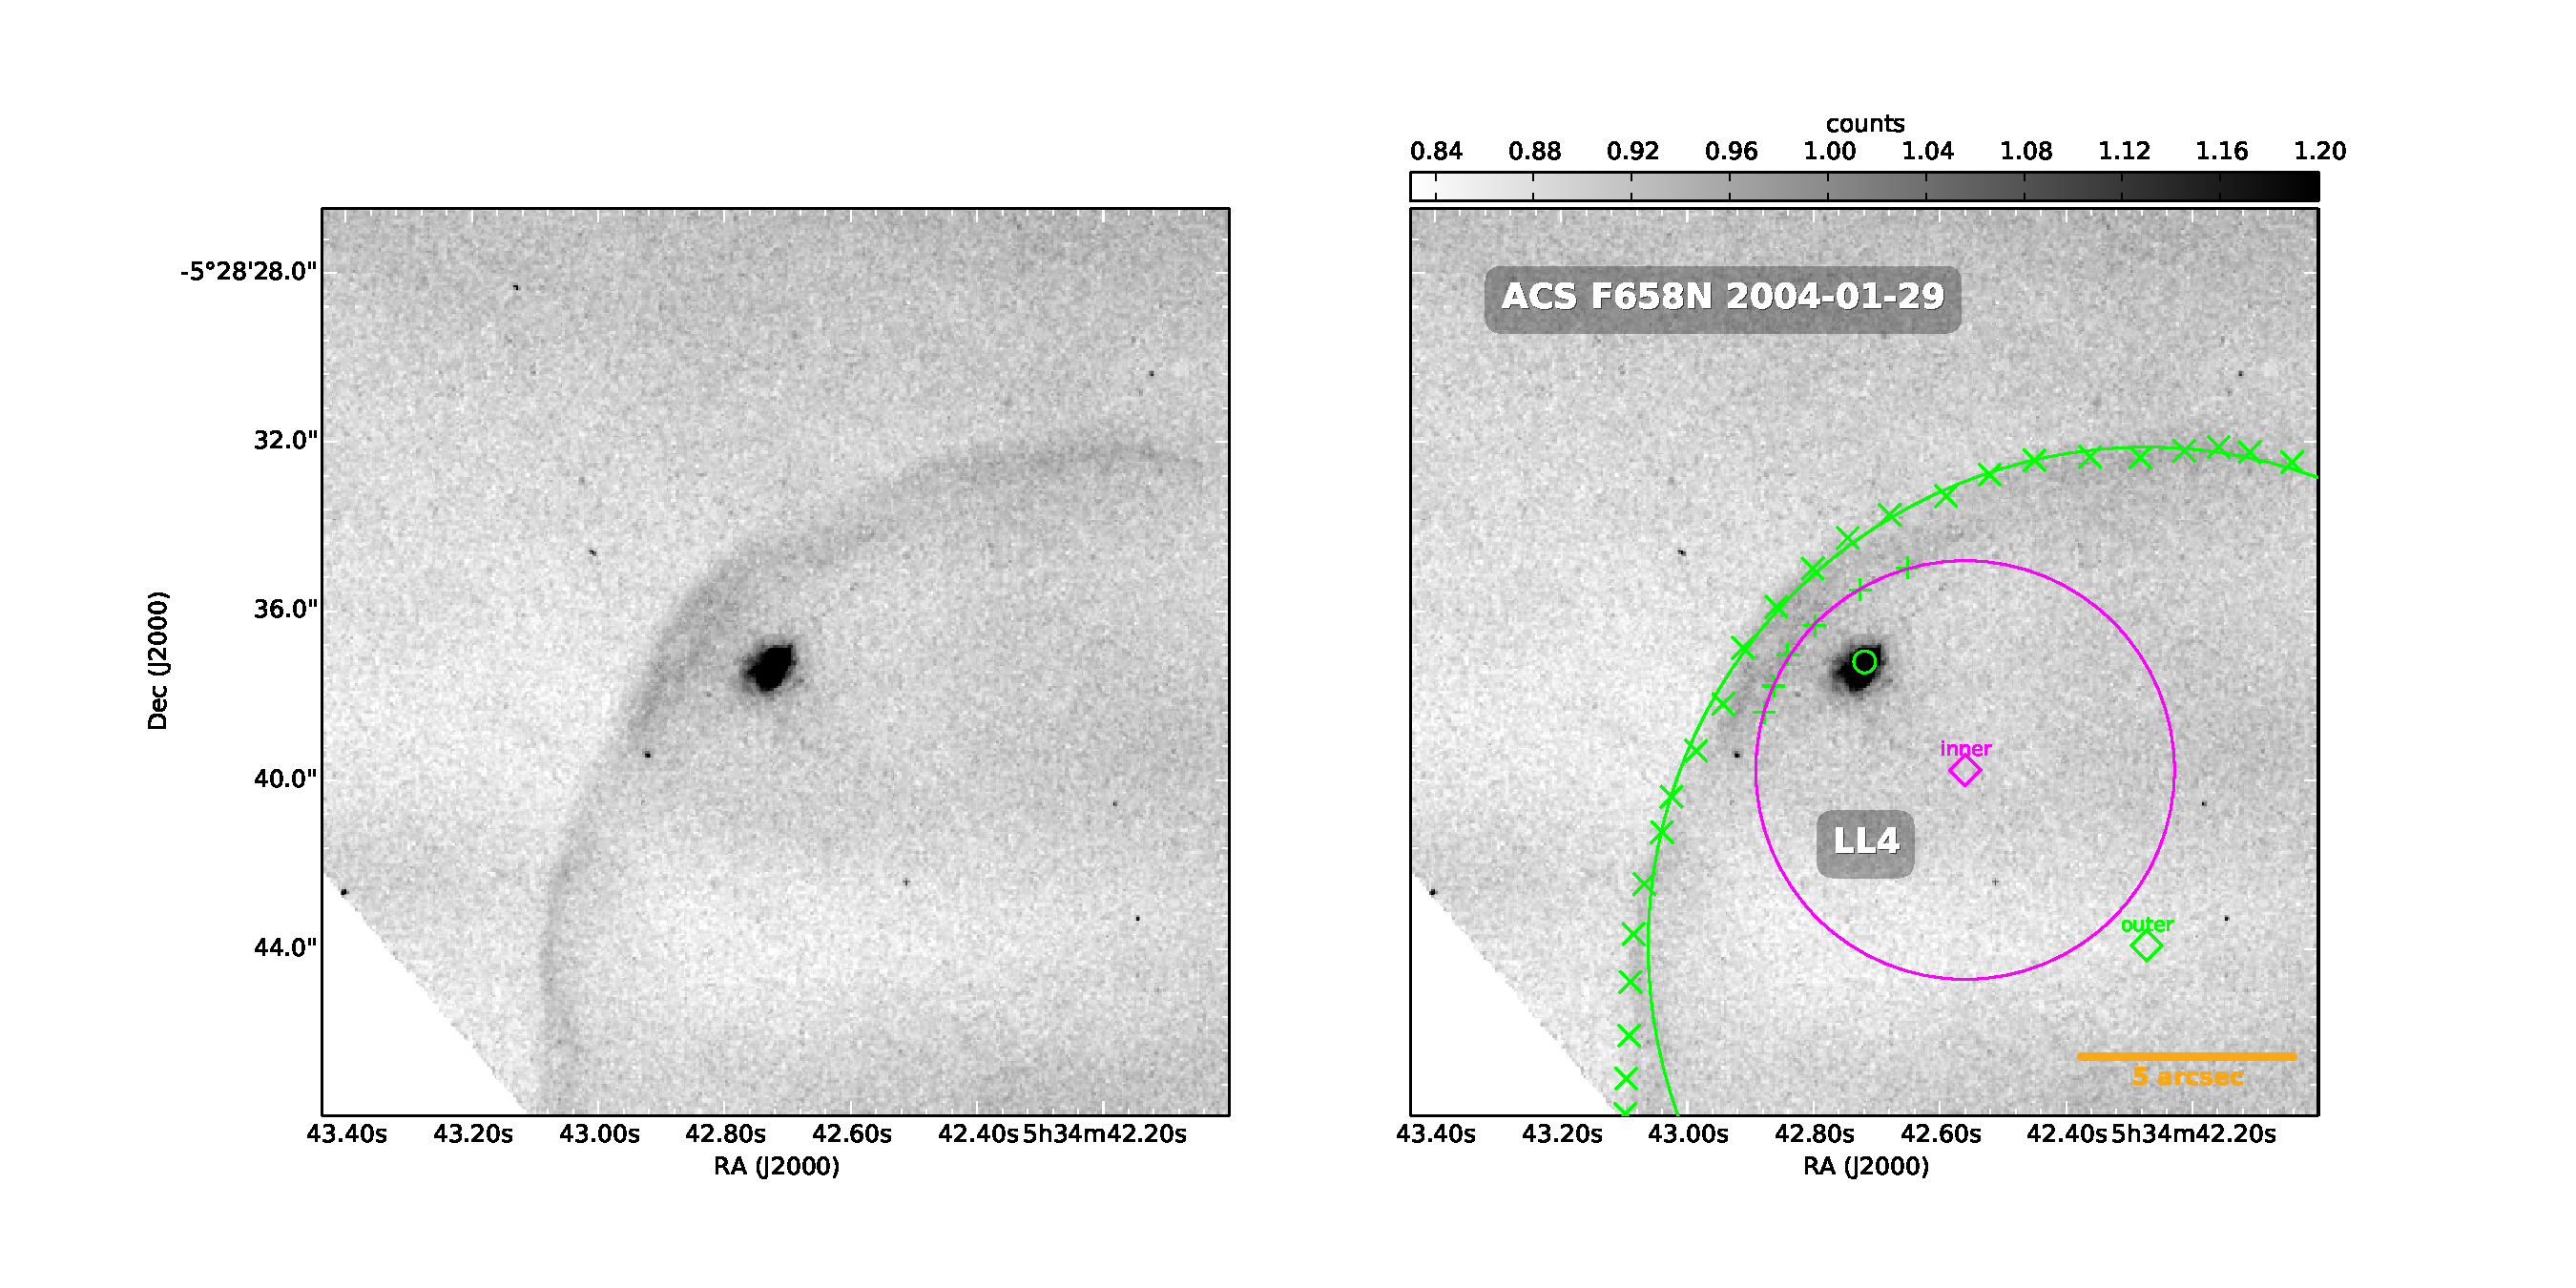
\includegraphics[width=0.5\linewidth]{./Figures/LL4-Bally_24-images} \\ 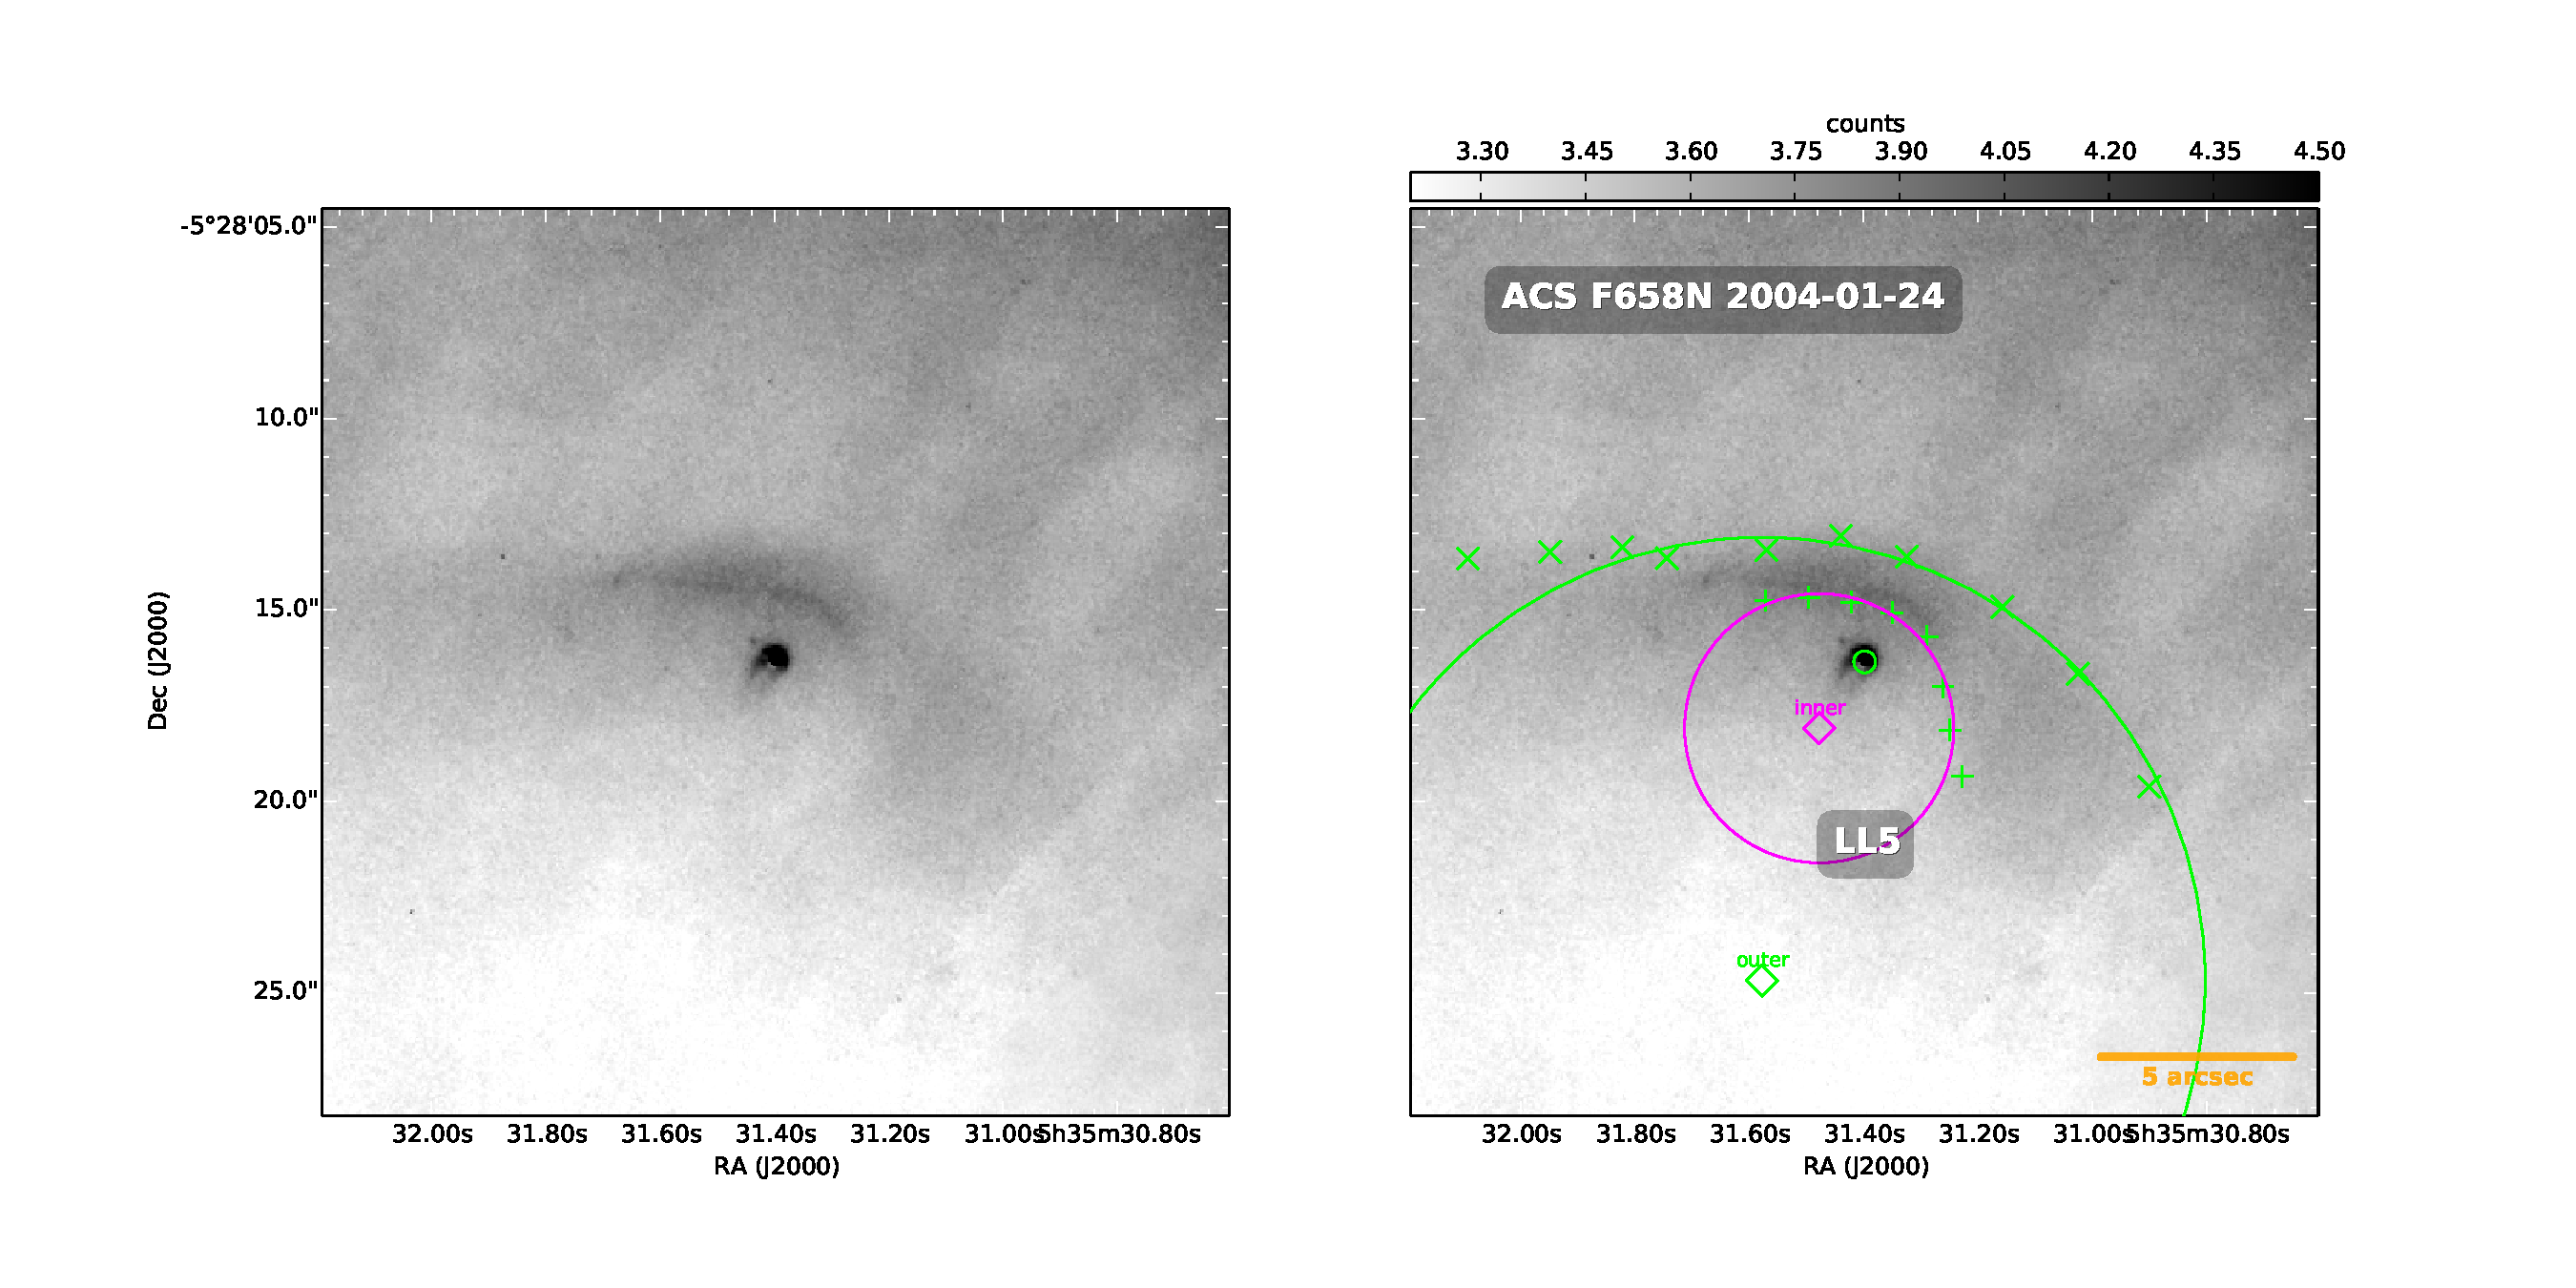
\includegraphics[width=0.5\linewidth]{./Figures/LL5-Bally_07-images} &
    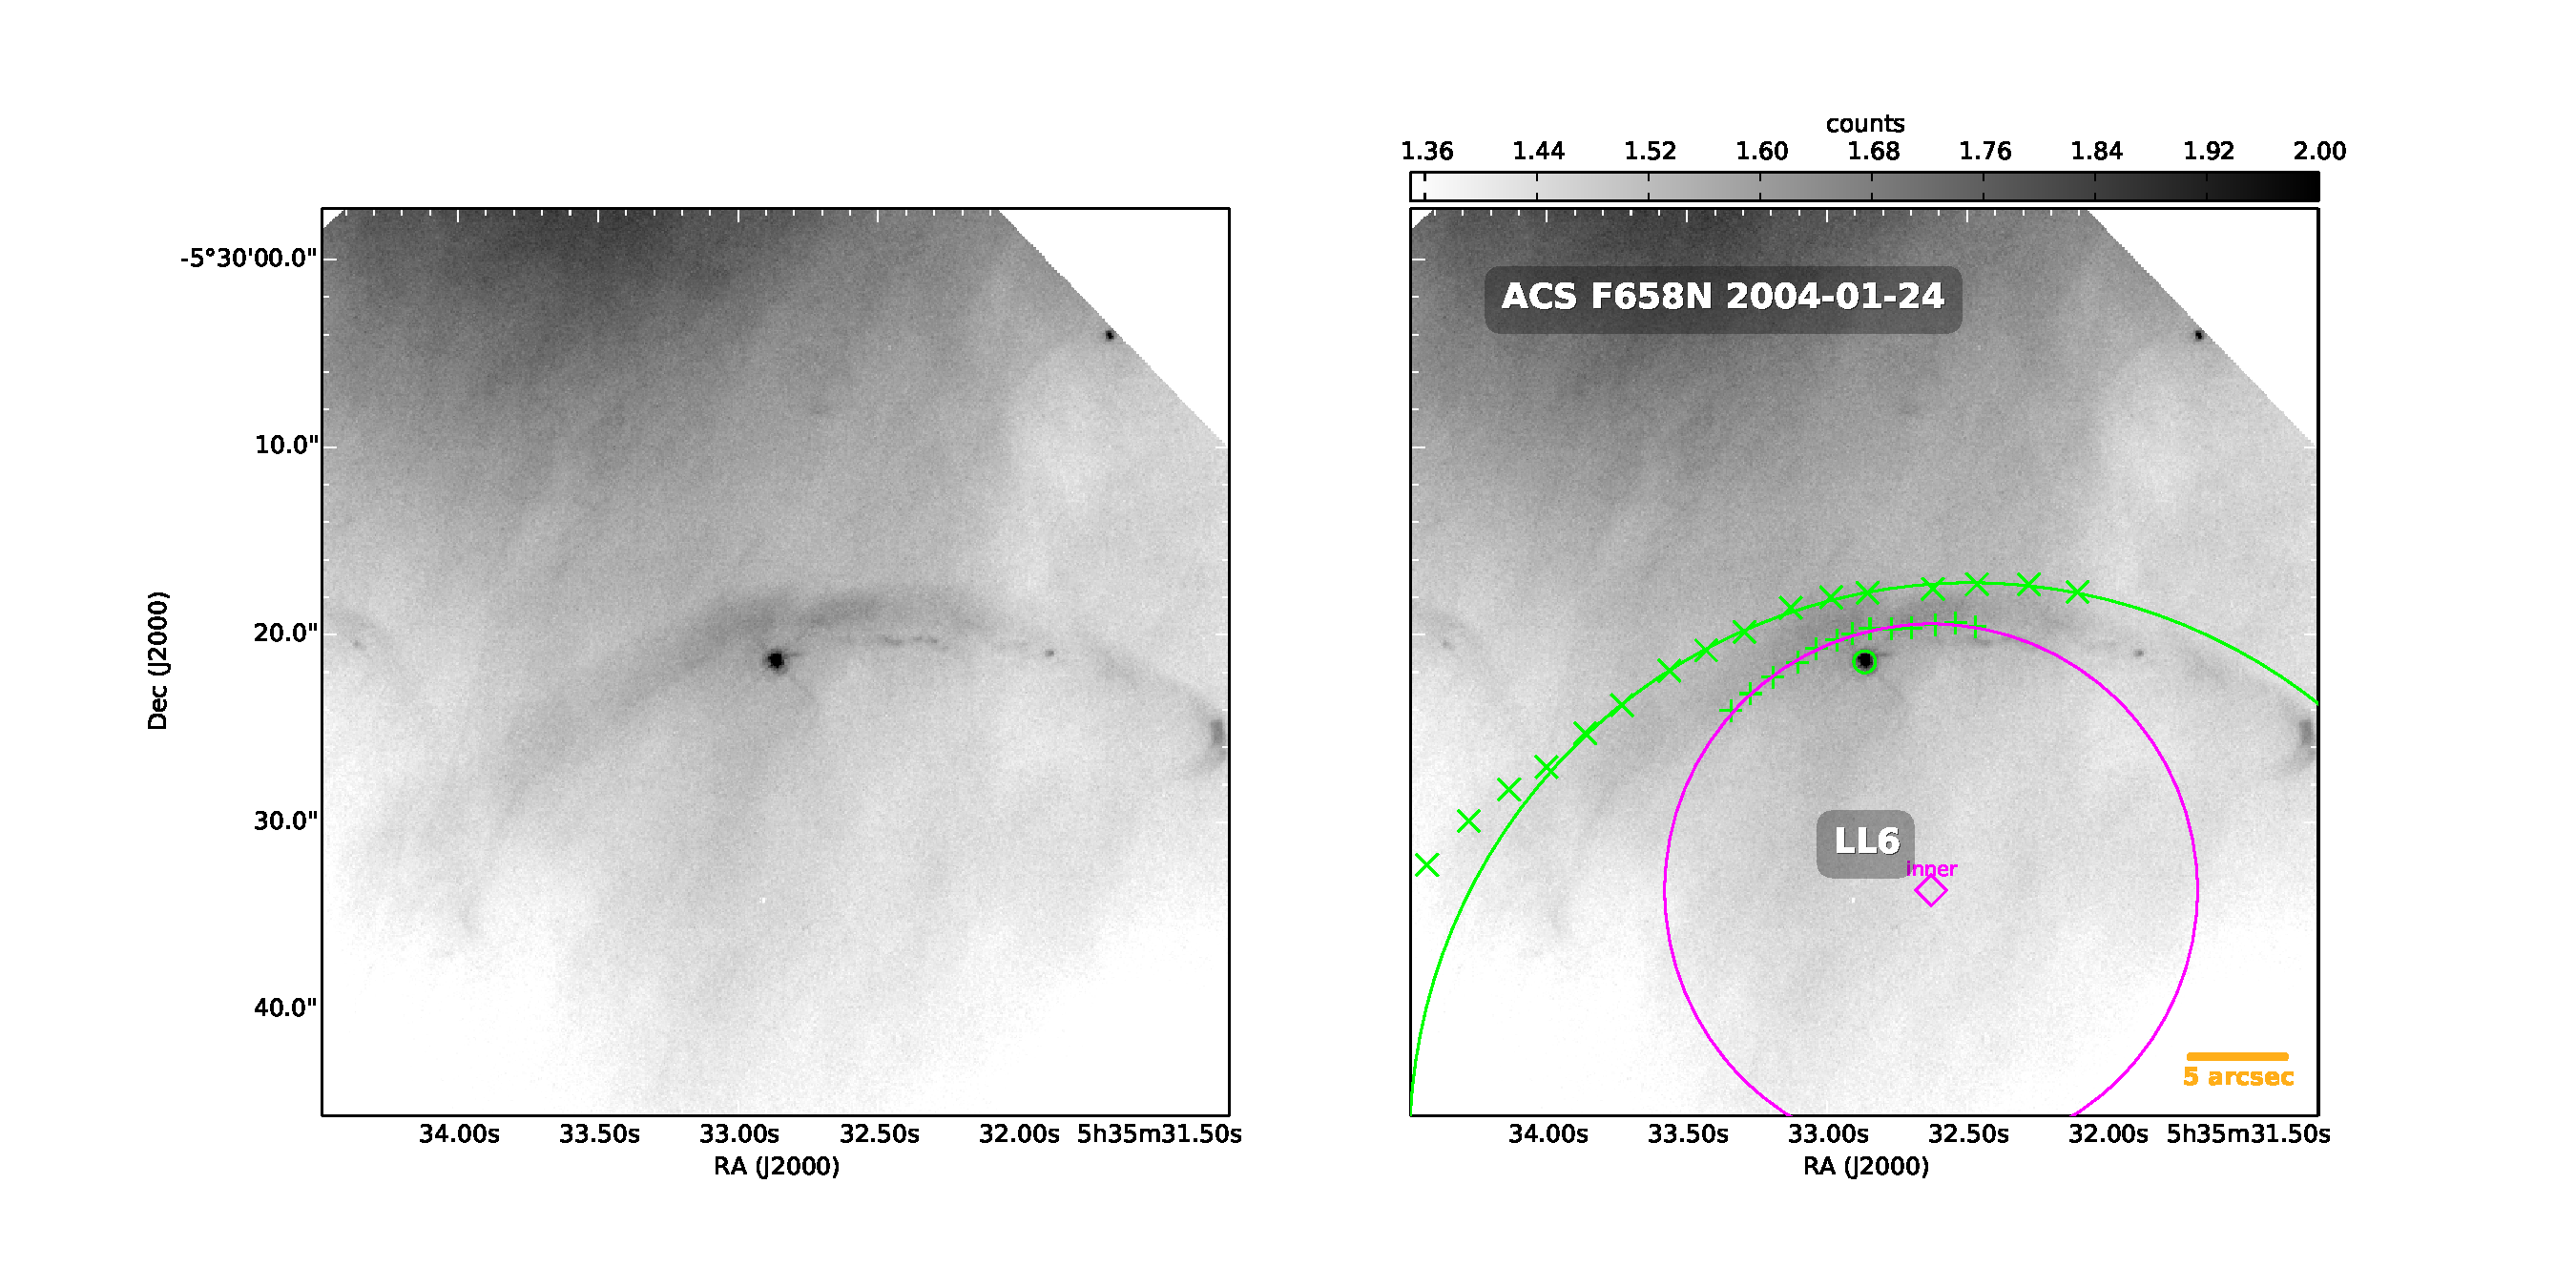
\includegraphics[width=0.5\linewidth]{./Figures/LL6-Bally_08-images} \\ 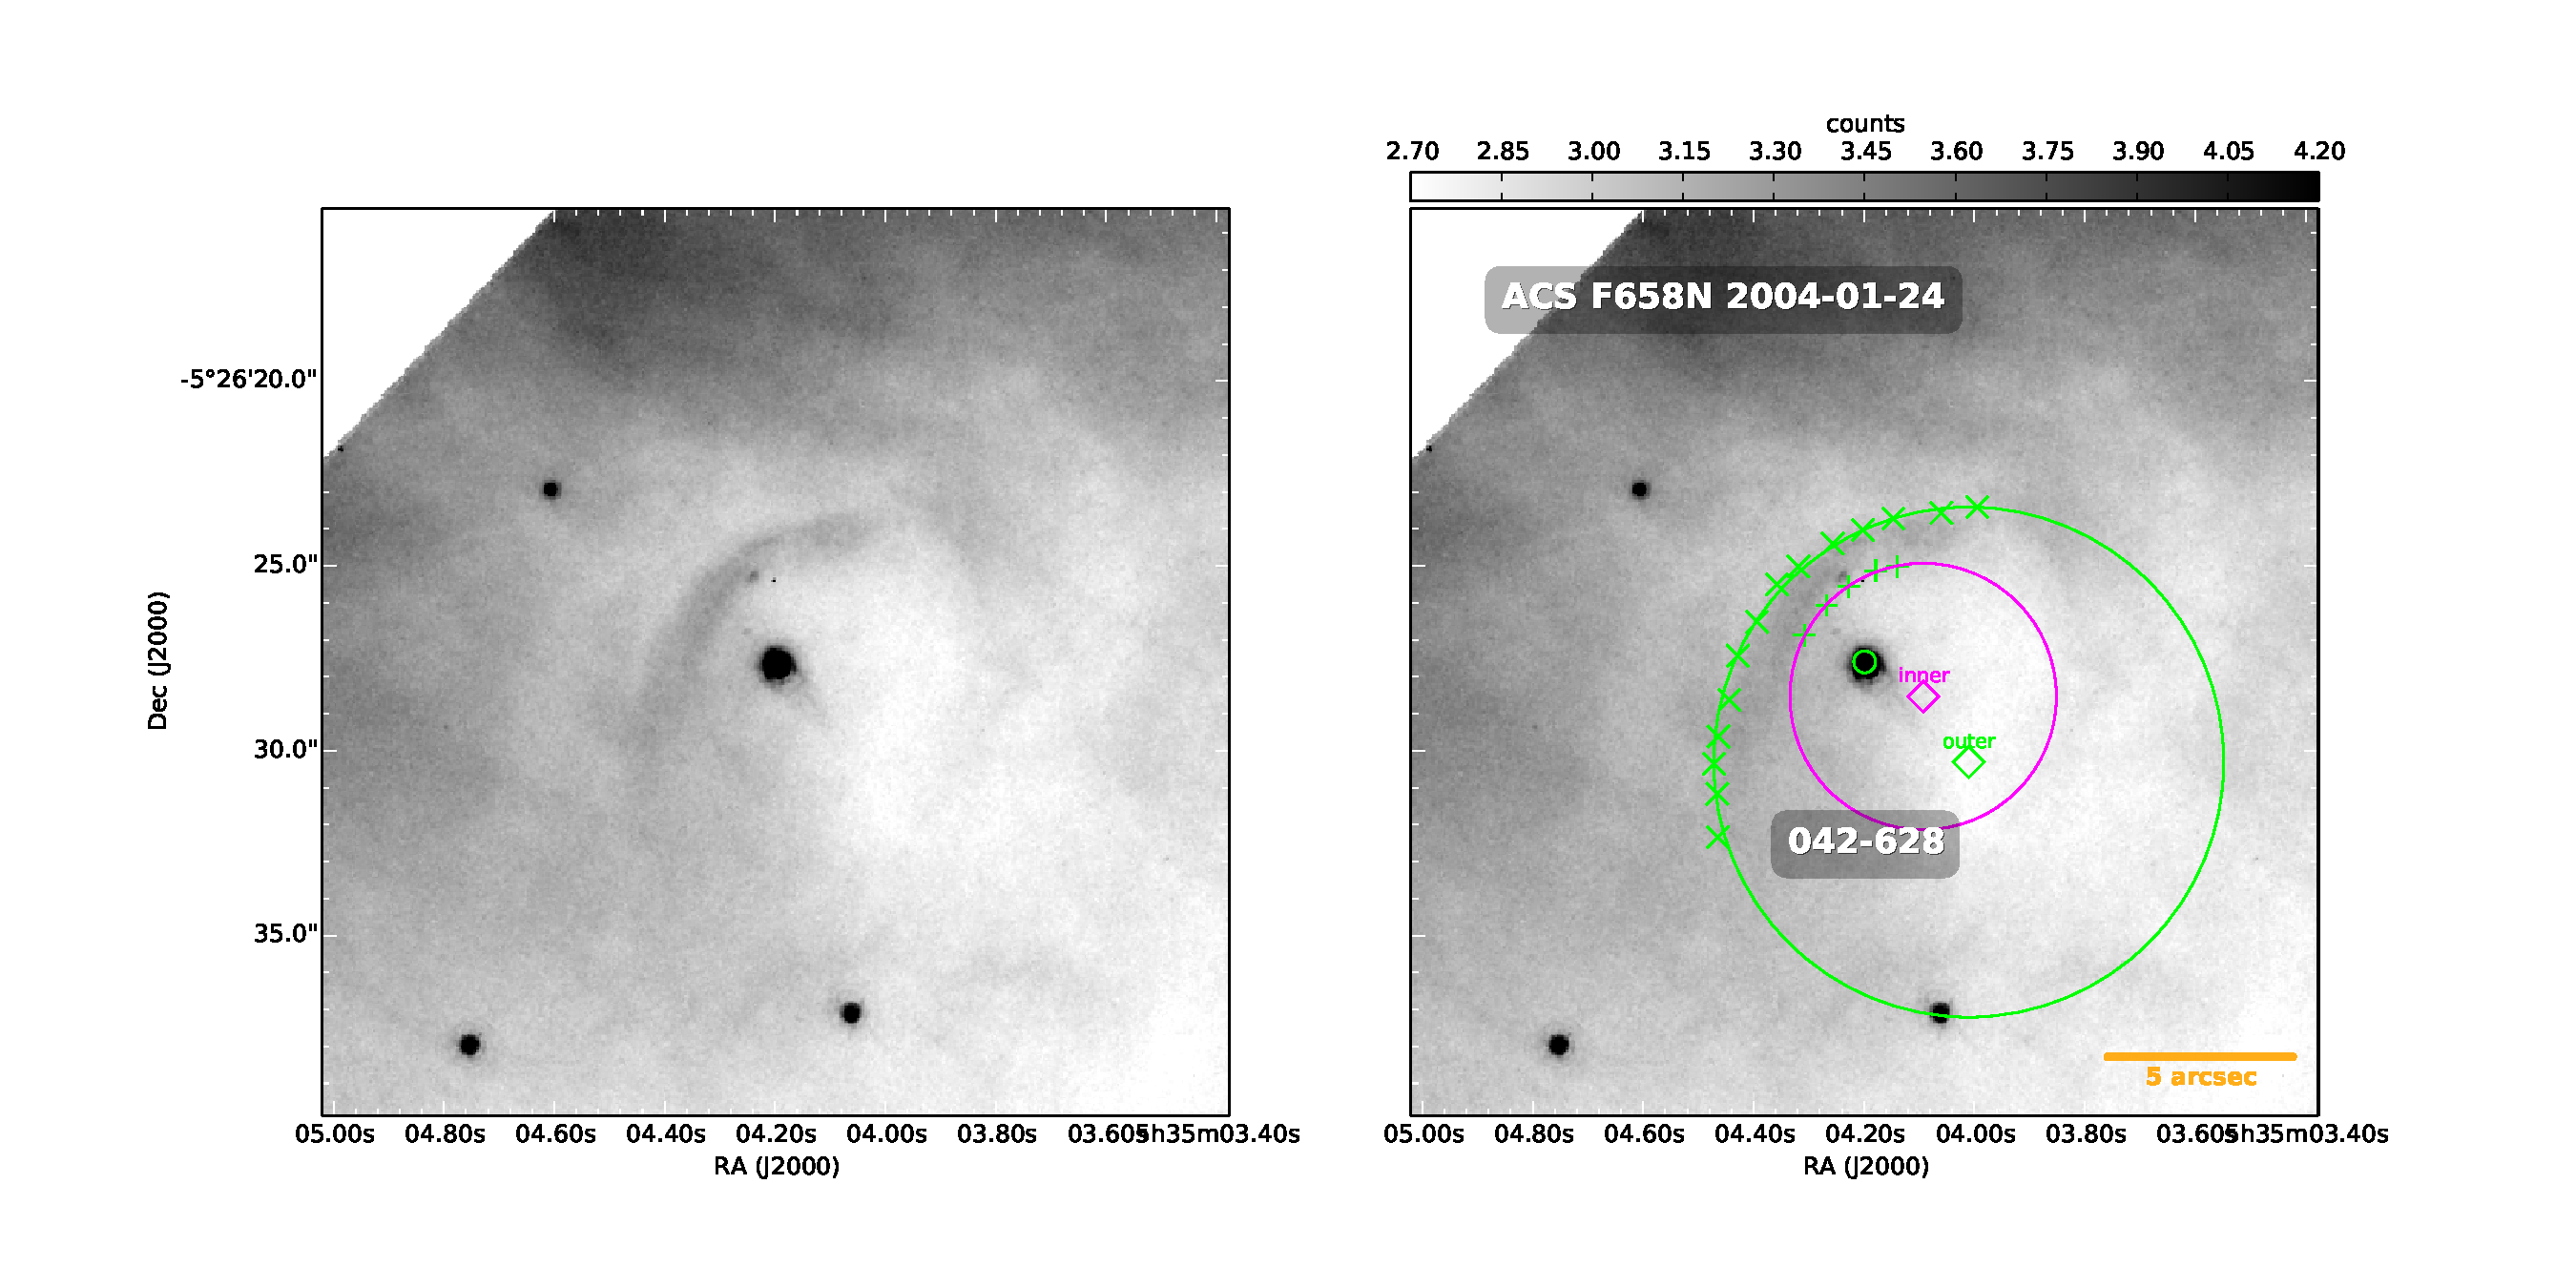
\includegraphics[width=0.5\linewidth]{./Figures/042-628-Bally_16-images} & 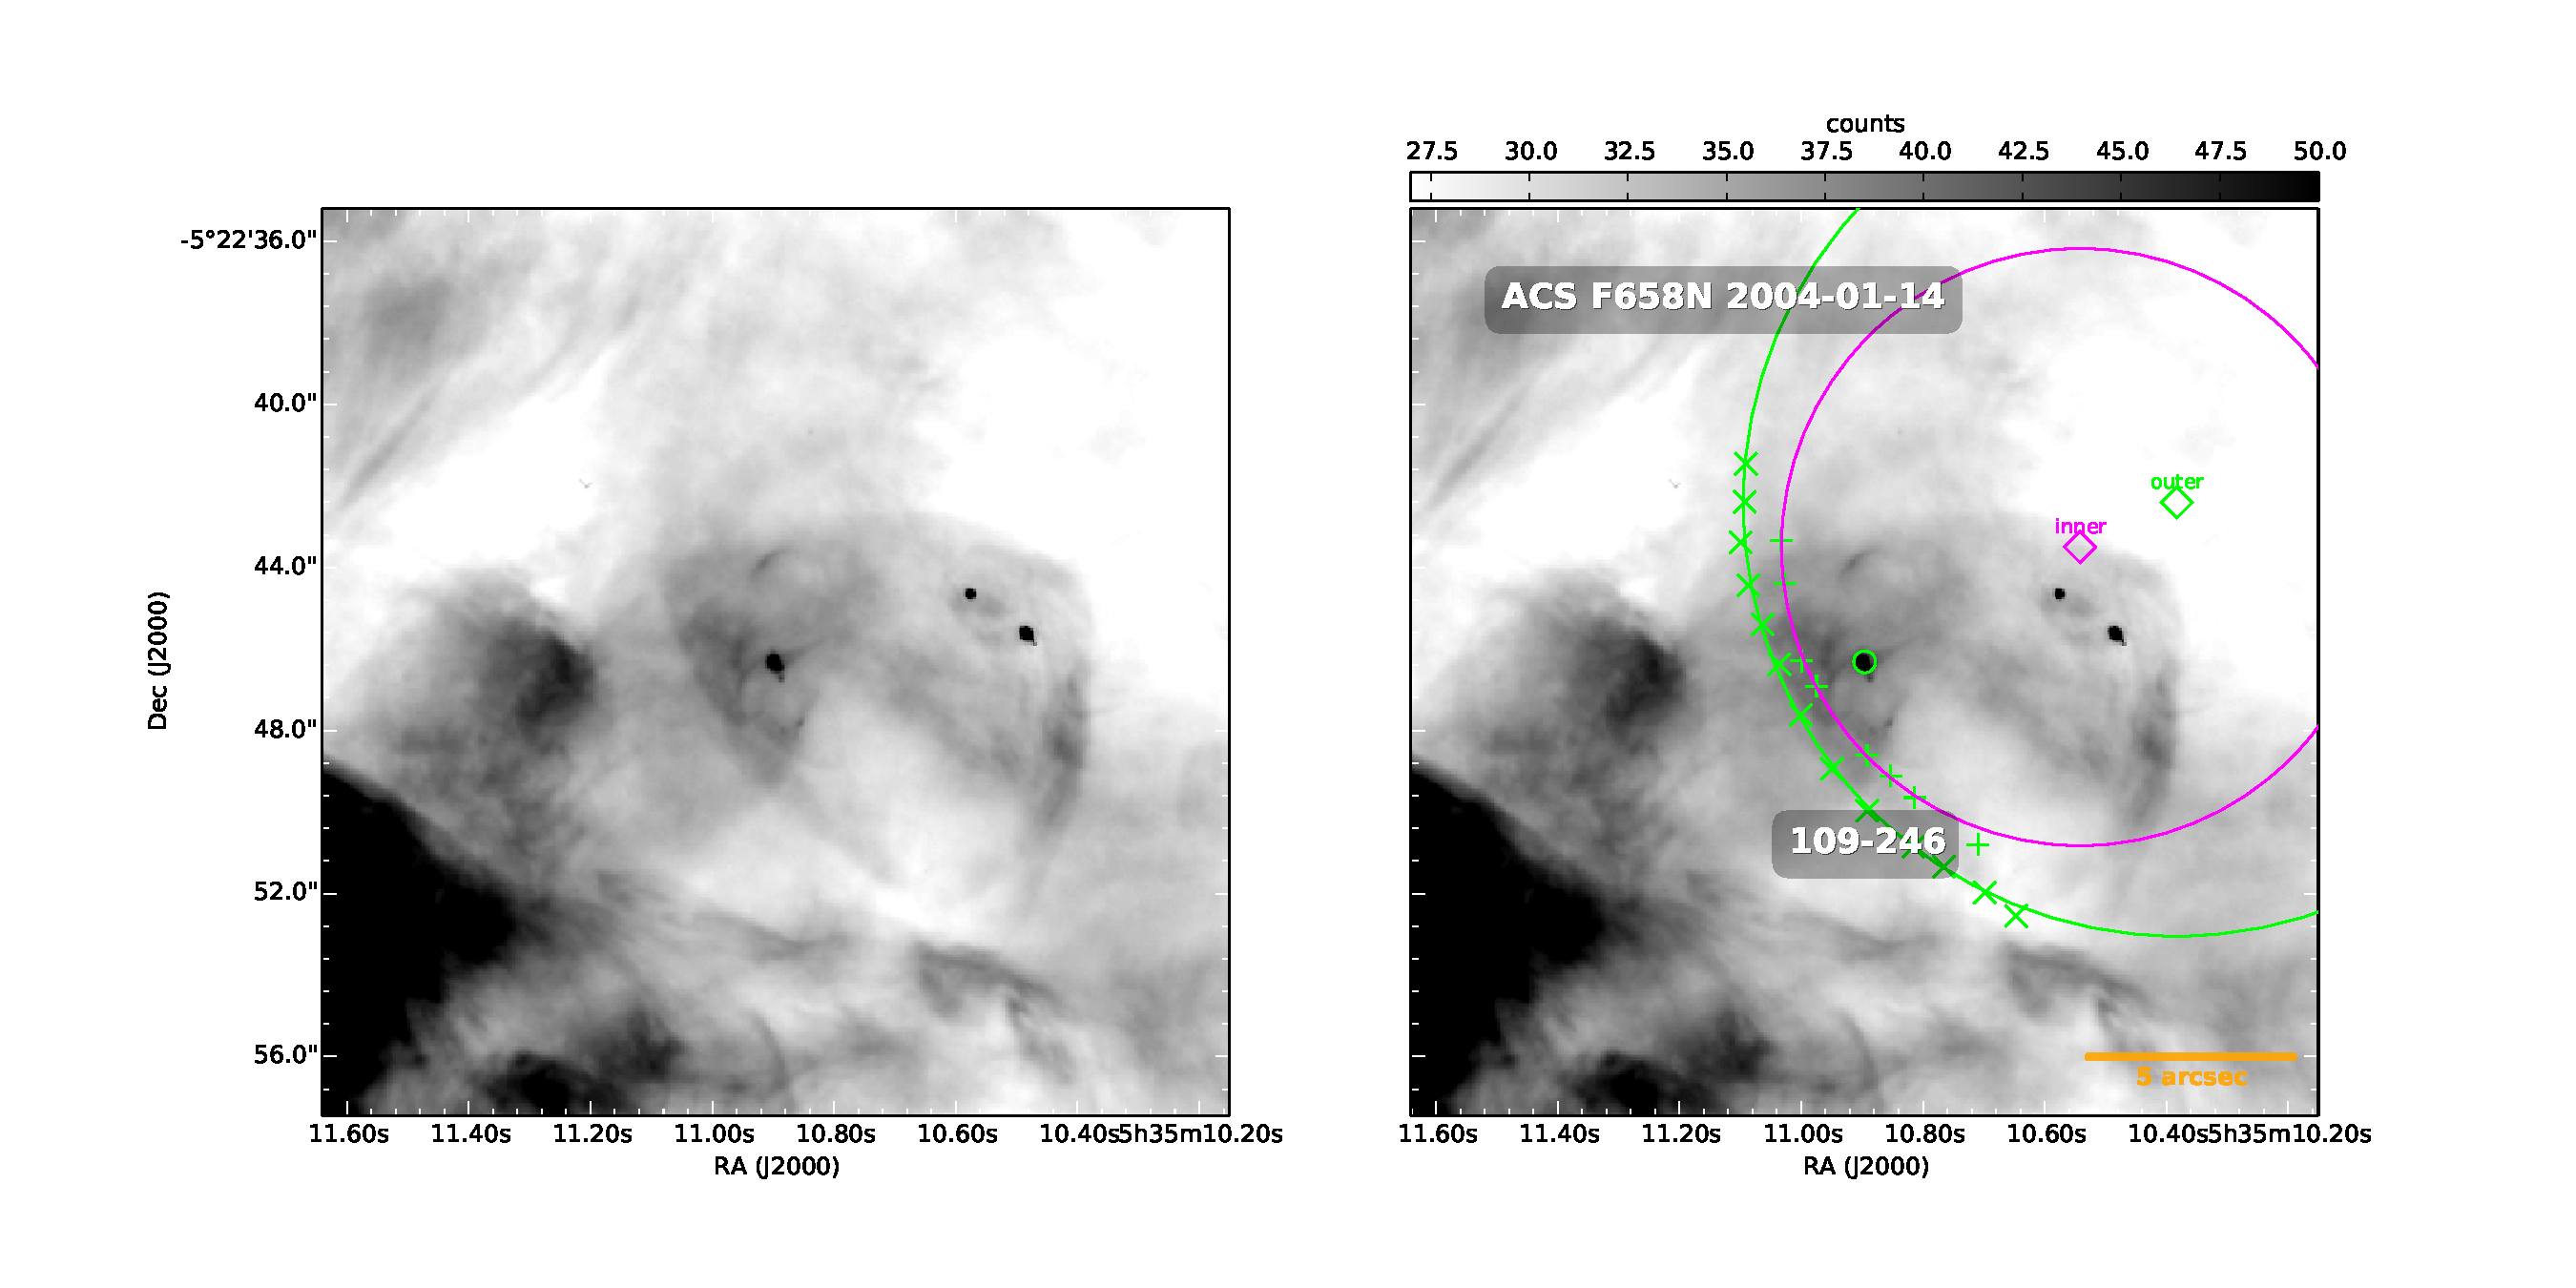
\includegraphics[width=0.5\linewidth]{./Figures/109-246-Bally_01-images} 
  \end{tabular}
  \caption{Ejemplos de objetos LL obtenidos del catálogo de \citet{Gutierrez-Soto:2015a}. A la derecha de cada panel se observa el objeto con las mediciones superpuestas de los radios característicos $(R'_0, R'_c)$ para las cáscaras exterior e interior o solo para una dependiendo del objeto. La escala de grises muestra el brillo, la barra amarilla indica la escala del objeto y las etiquetas mestran el nombre del objeto, el instrumento que se utilizó para obtener la imagen y la fecha en que se obtuvo.}
  \label{fig:Luis-mosaic-1}
\end{figure}


\begin{figure}
  \centering
  \ContinuedFloat
    \captionsetup{list=off,format=cont}
  \begin{tabular}{cc}
    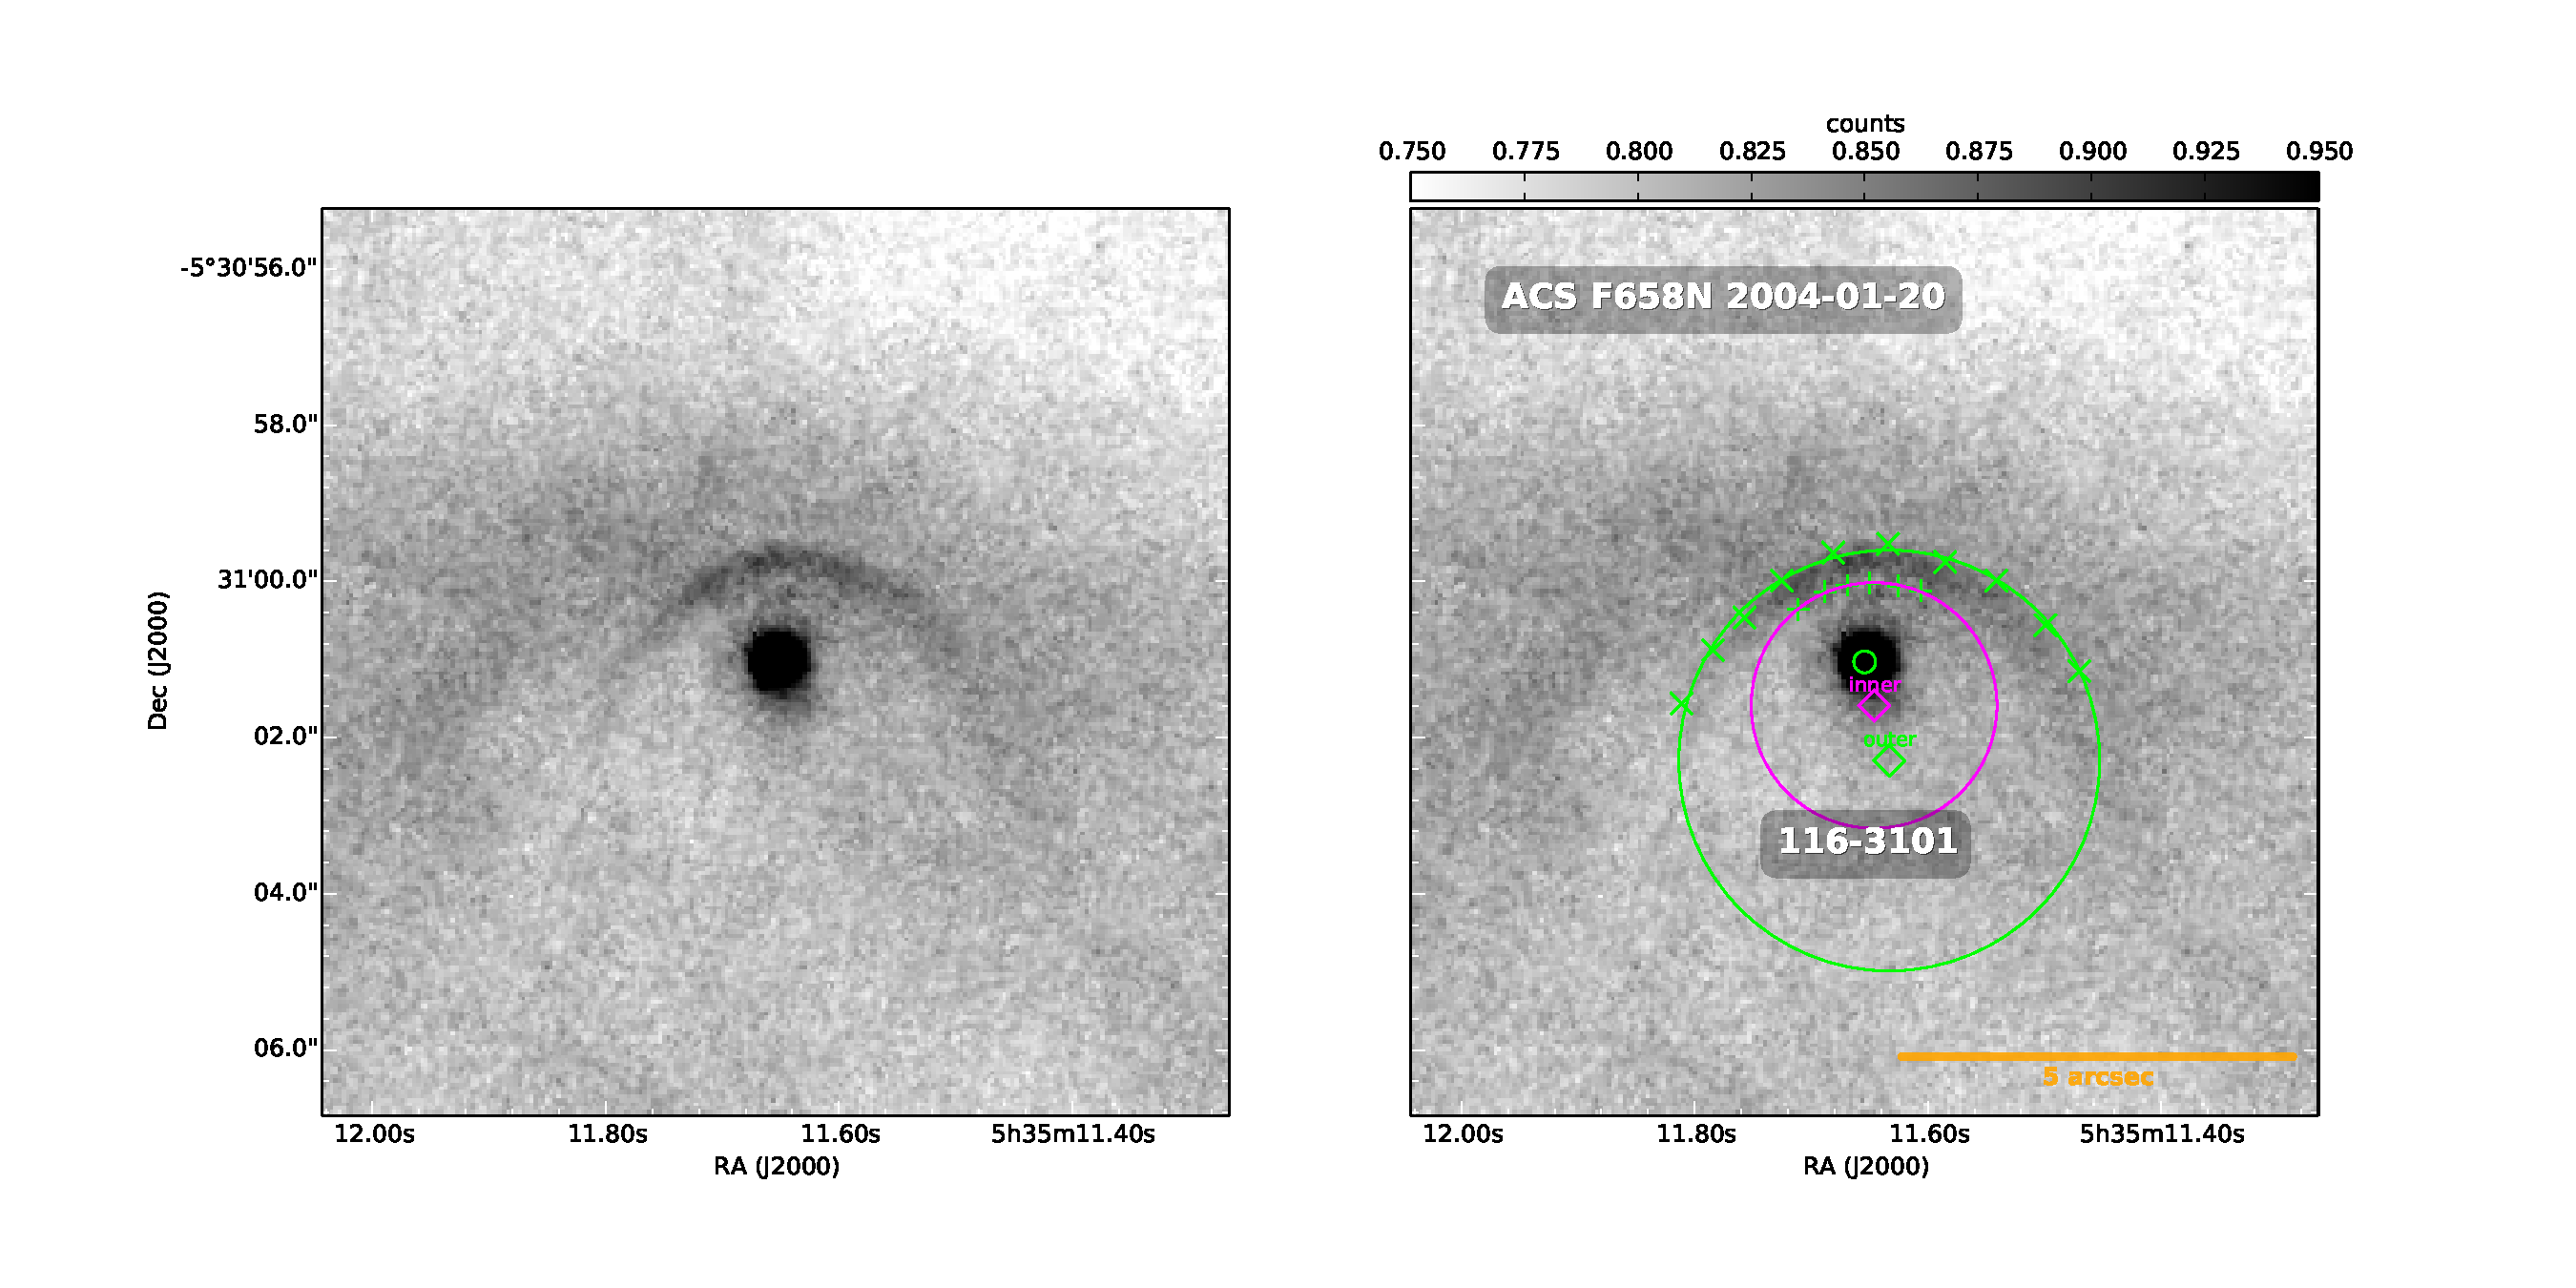
\includegraphics[width=0.5\linewidth]{./Figures/116-3101-Bally_14-images} & 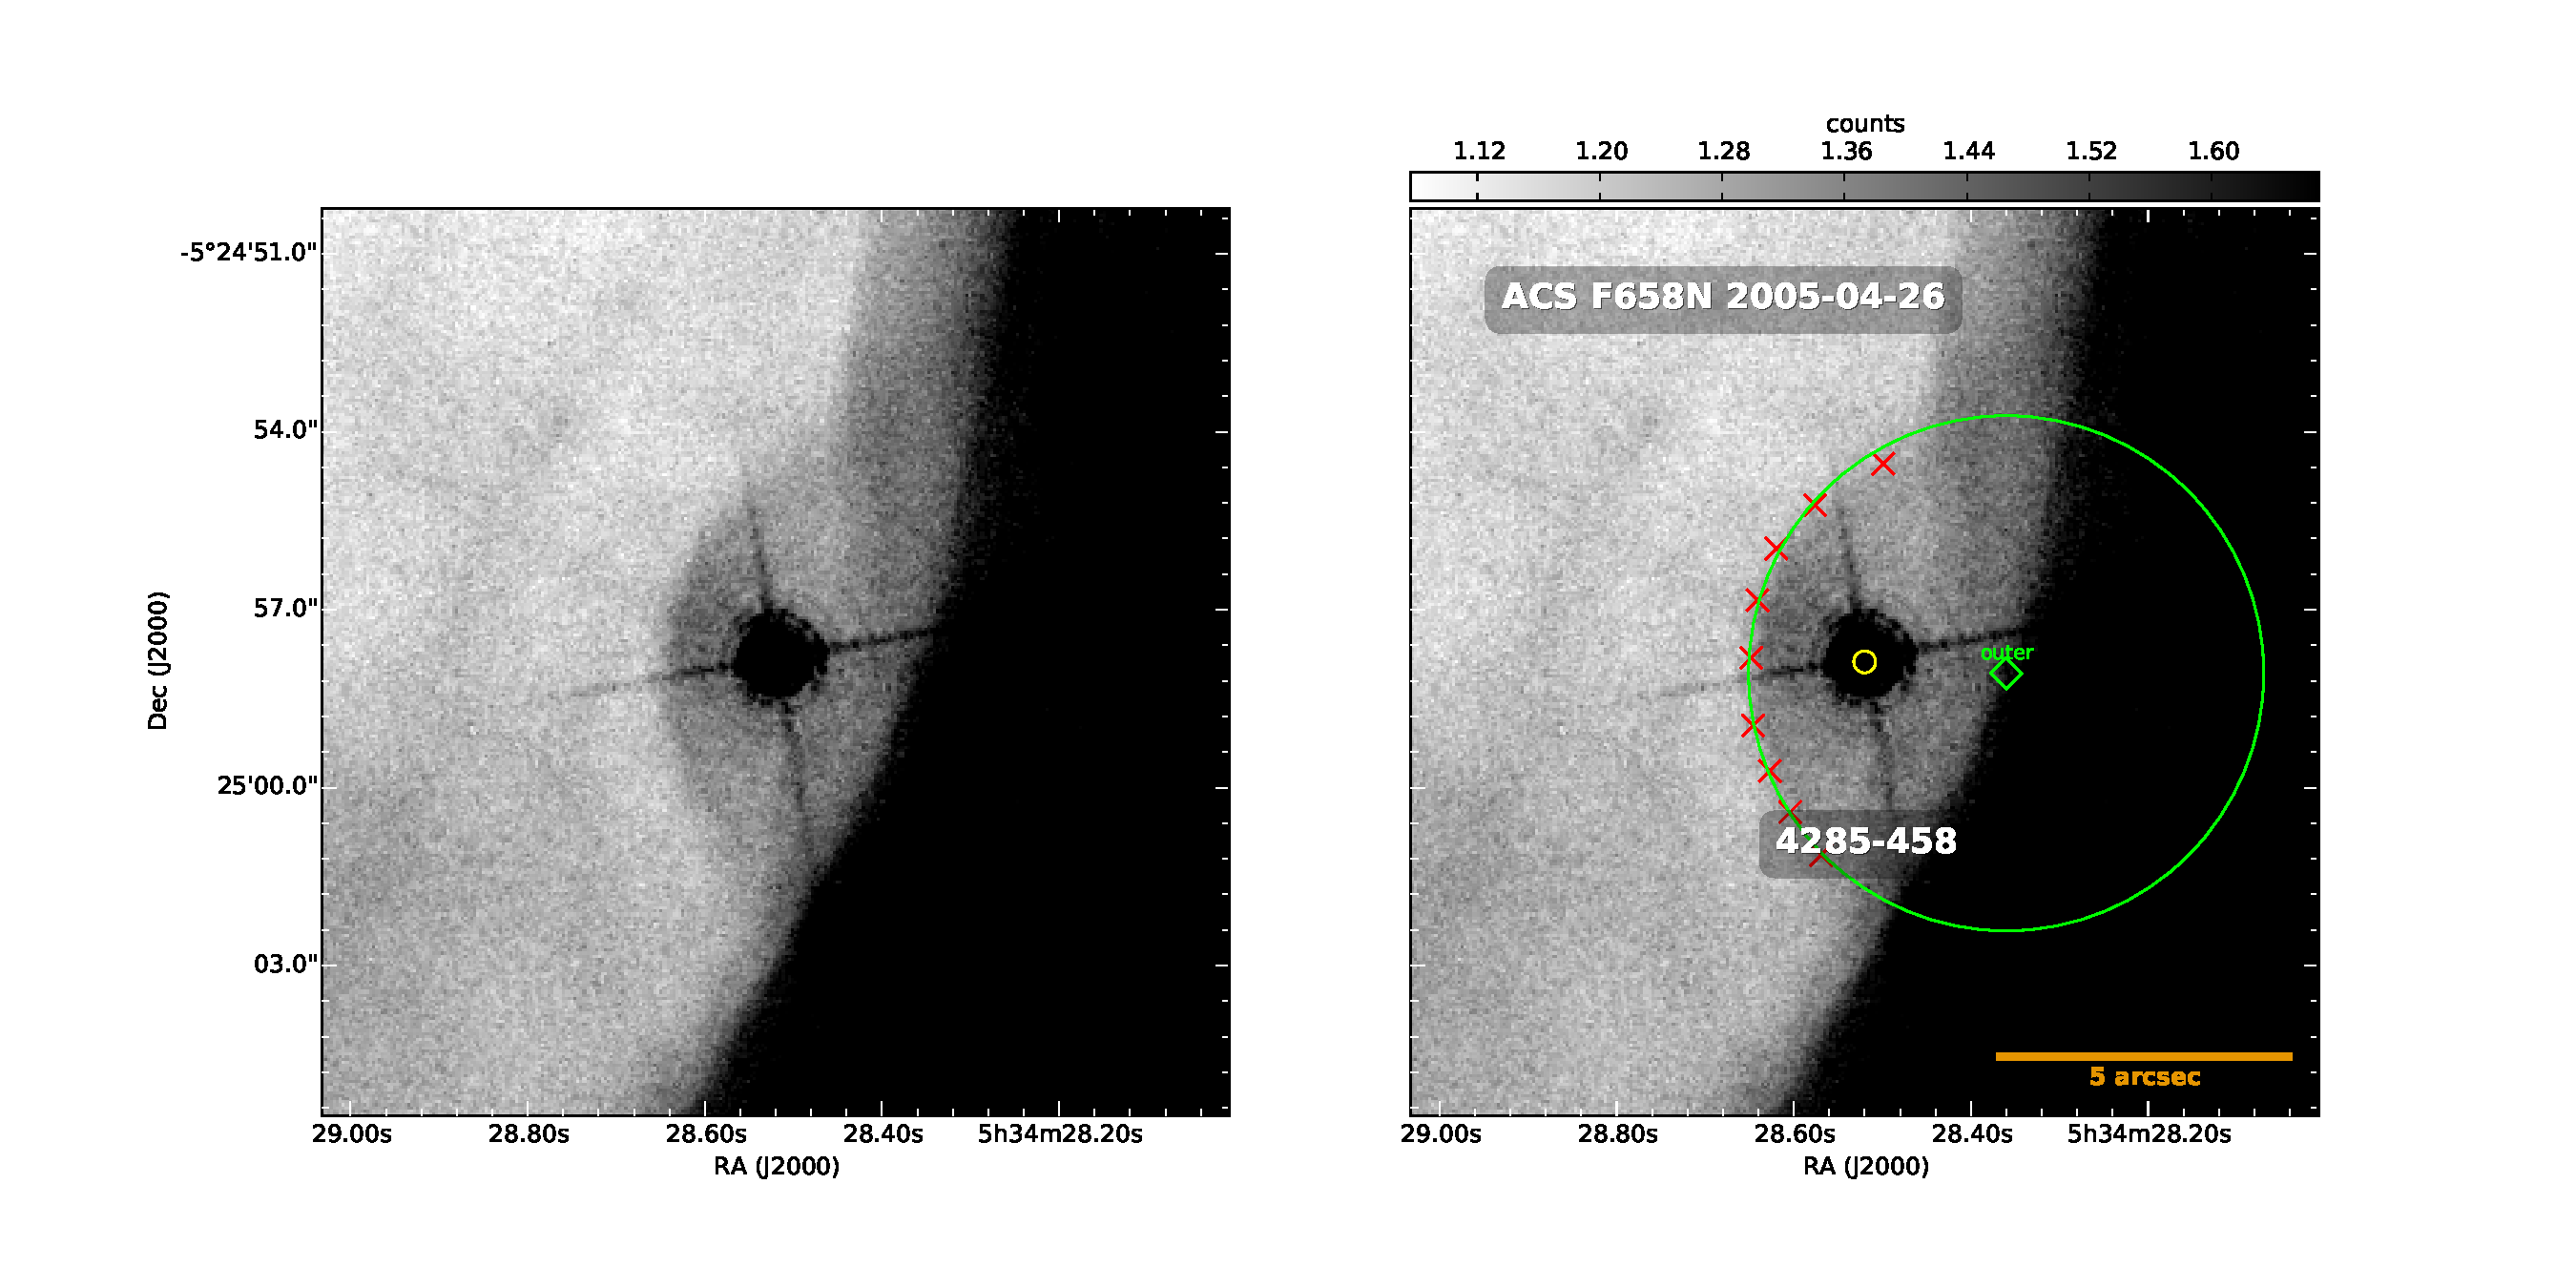
\includegraphics[width=0.5\linewidth]{./Figures/4285-458-Robberto_ACS_1r_f658n-images} \\ 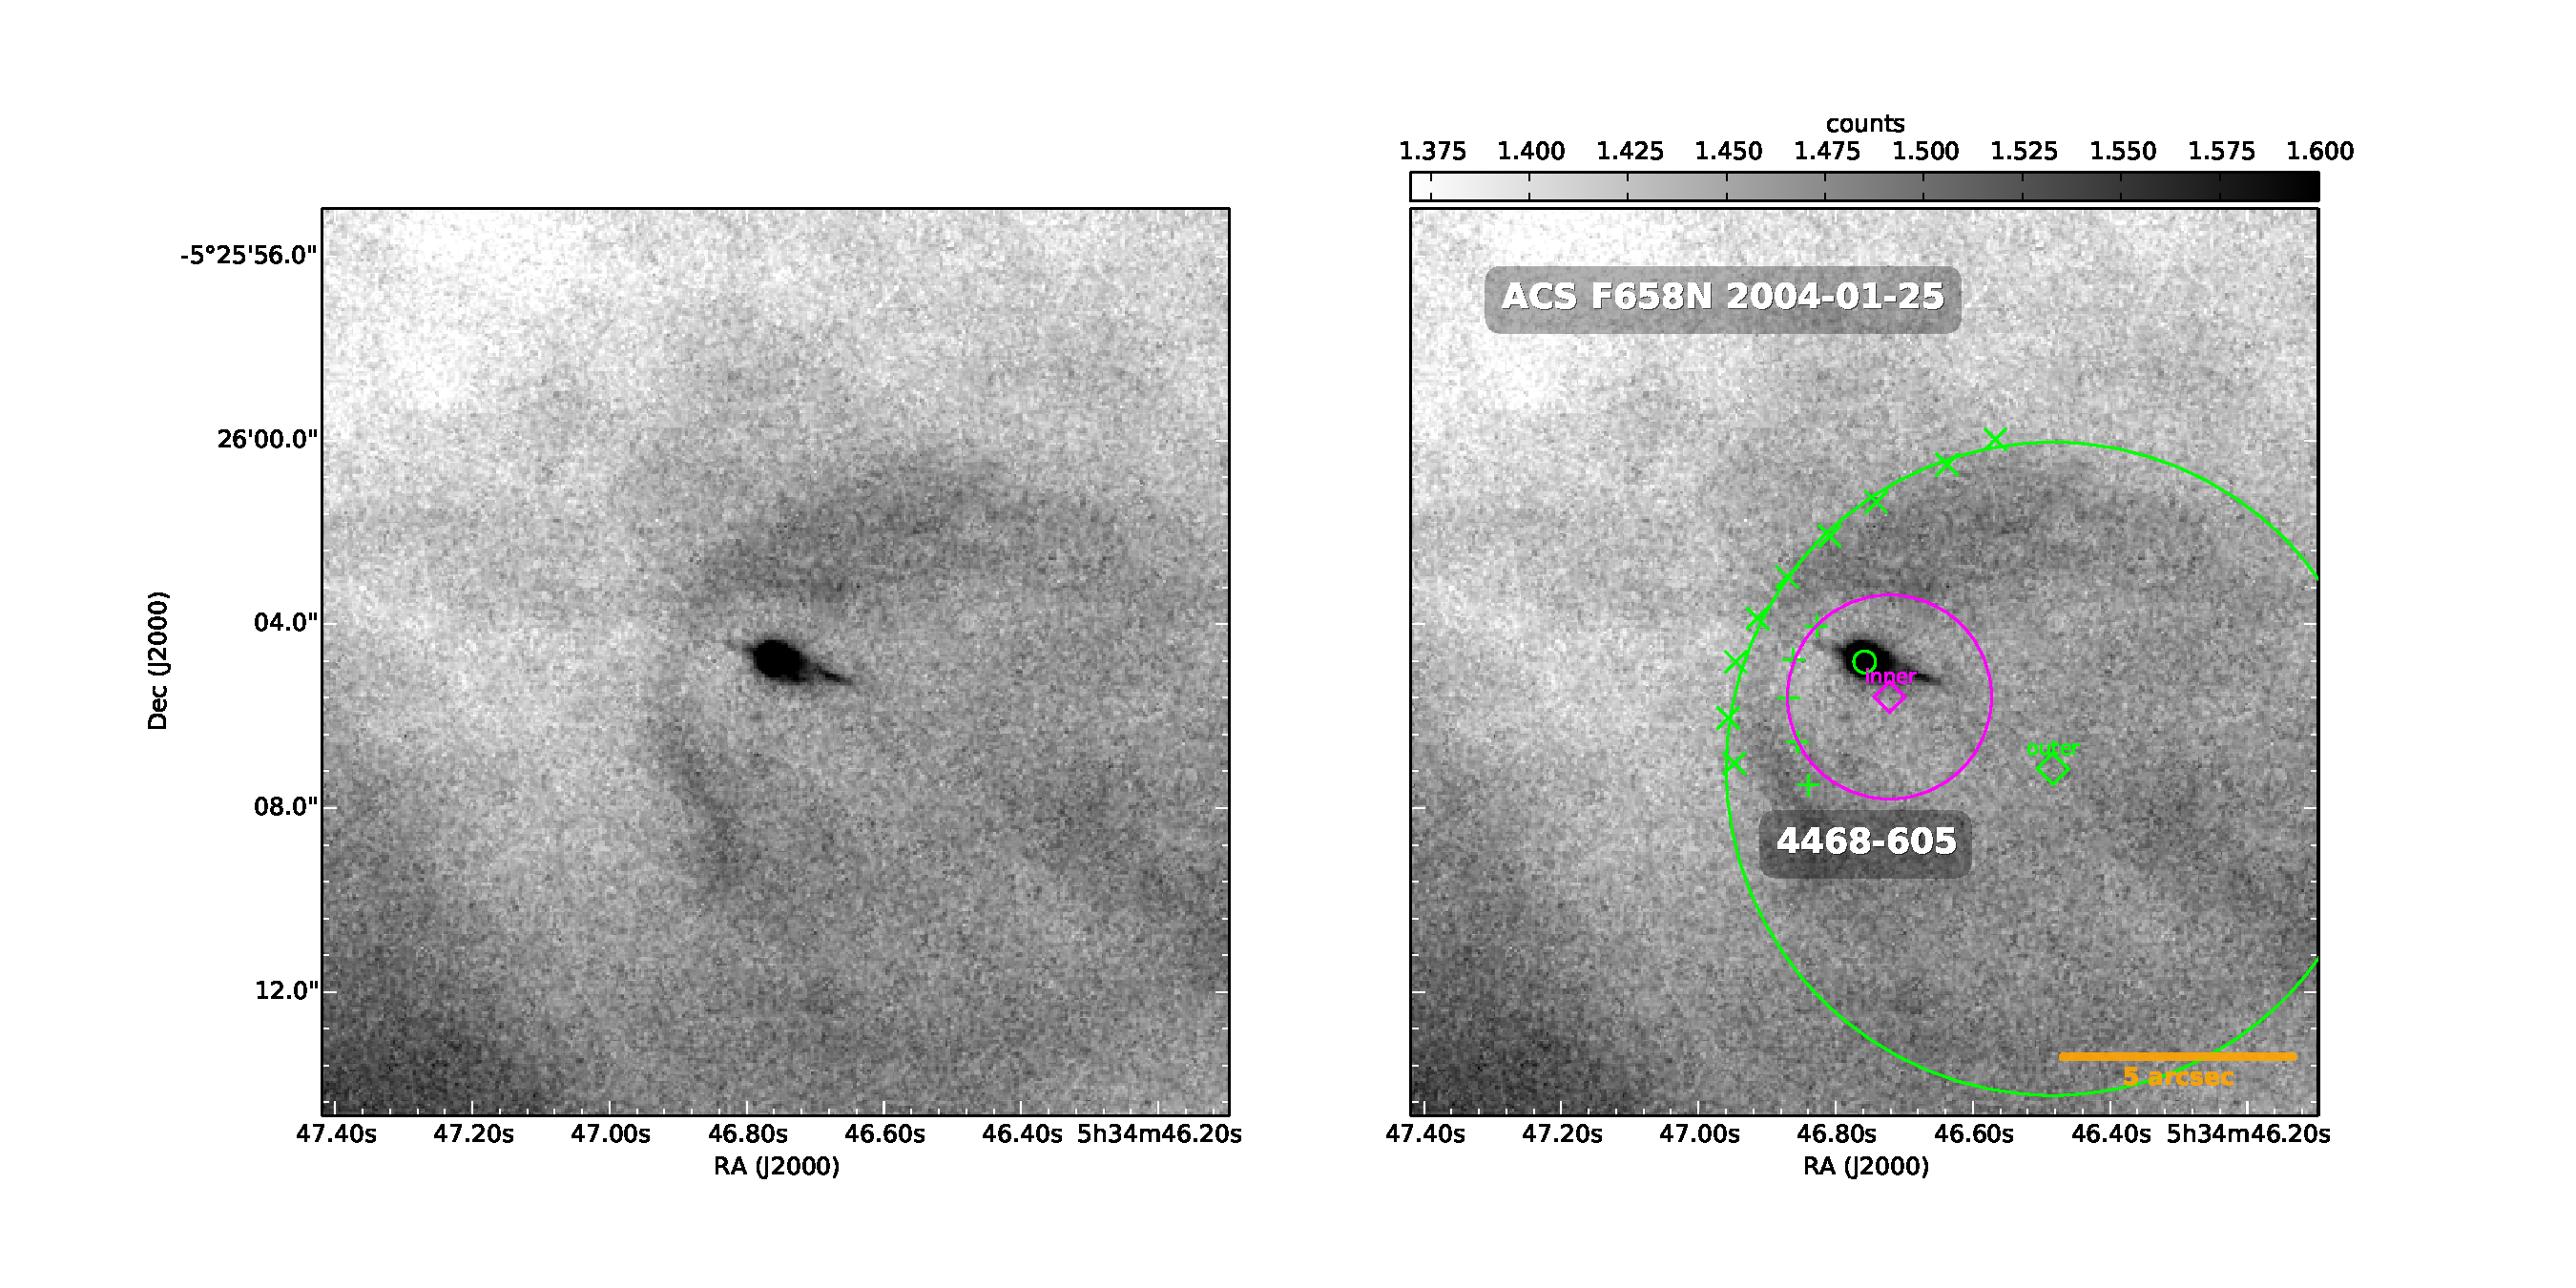
\includegraphics[width=0.5\linewidth]{./Figures/4468-605-Bally_17-images} &
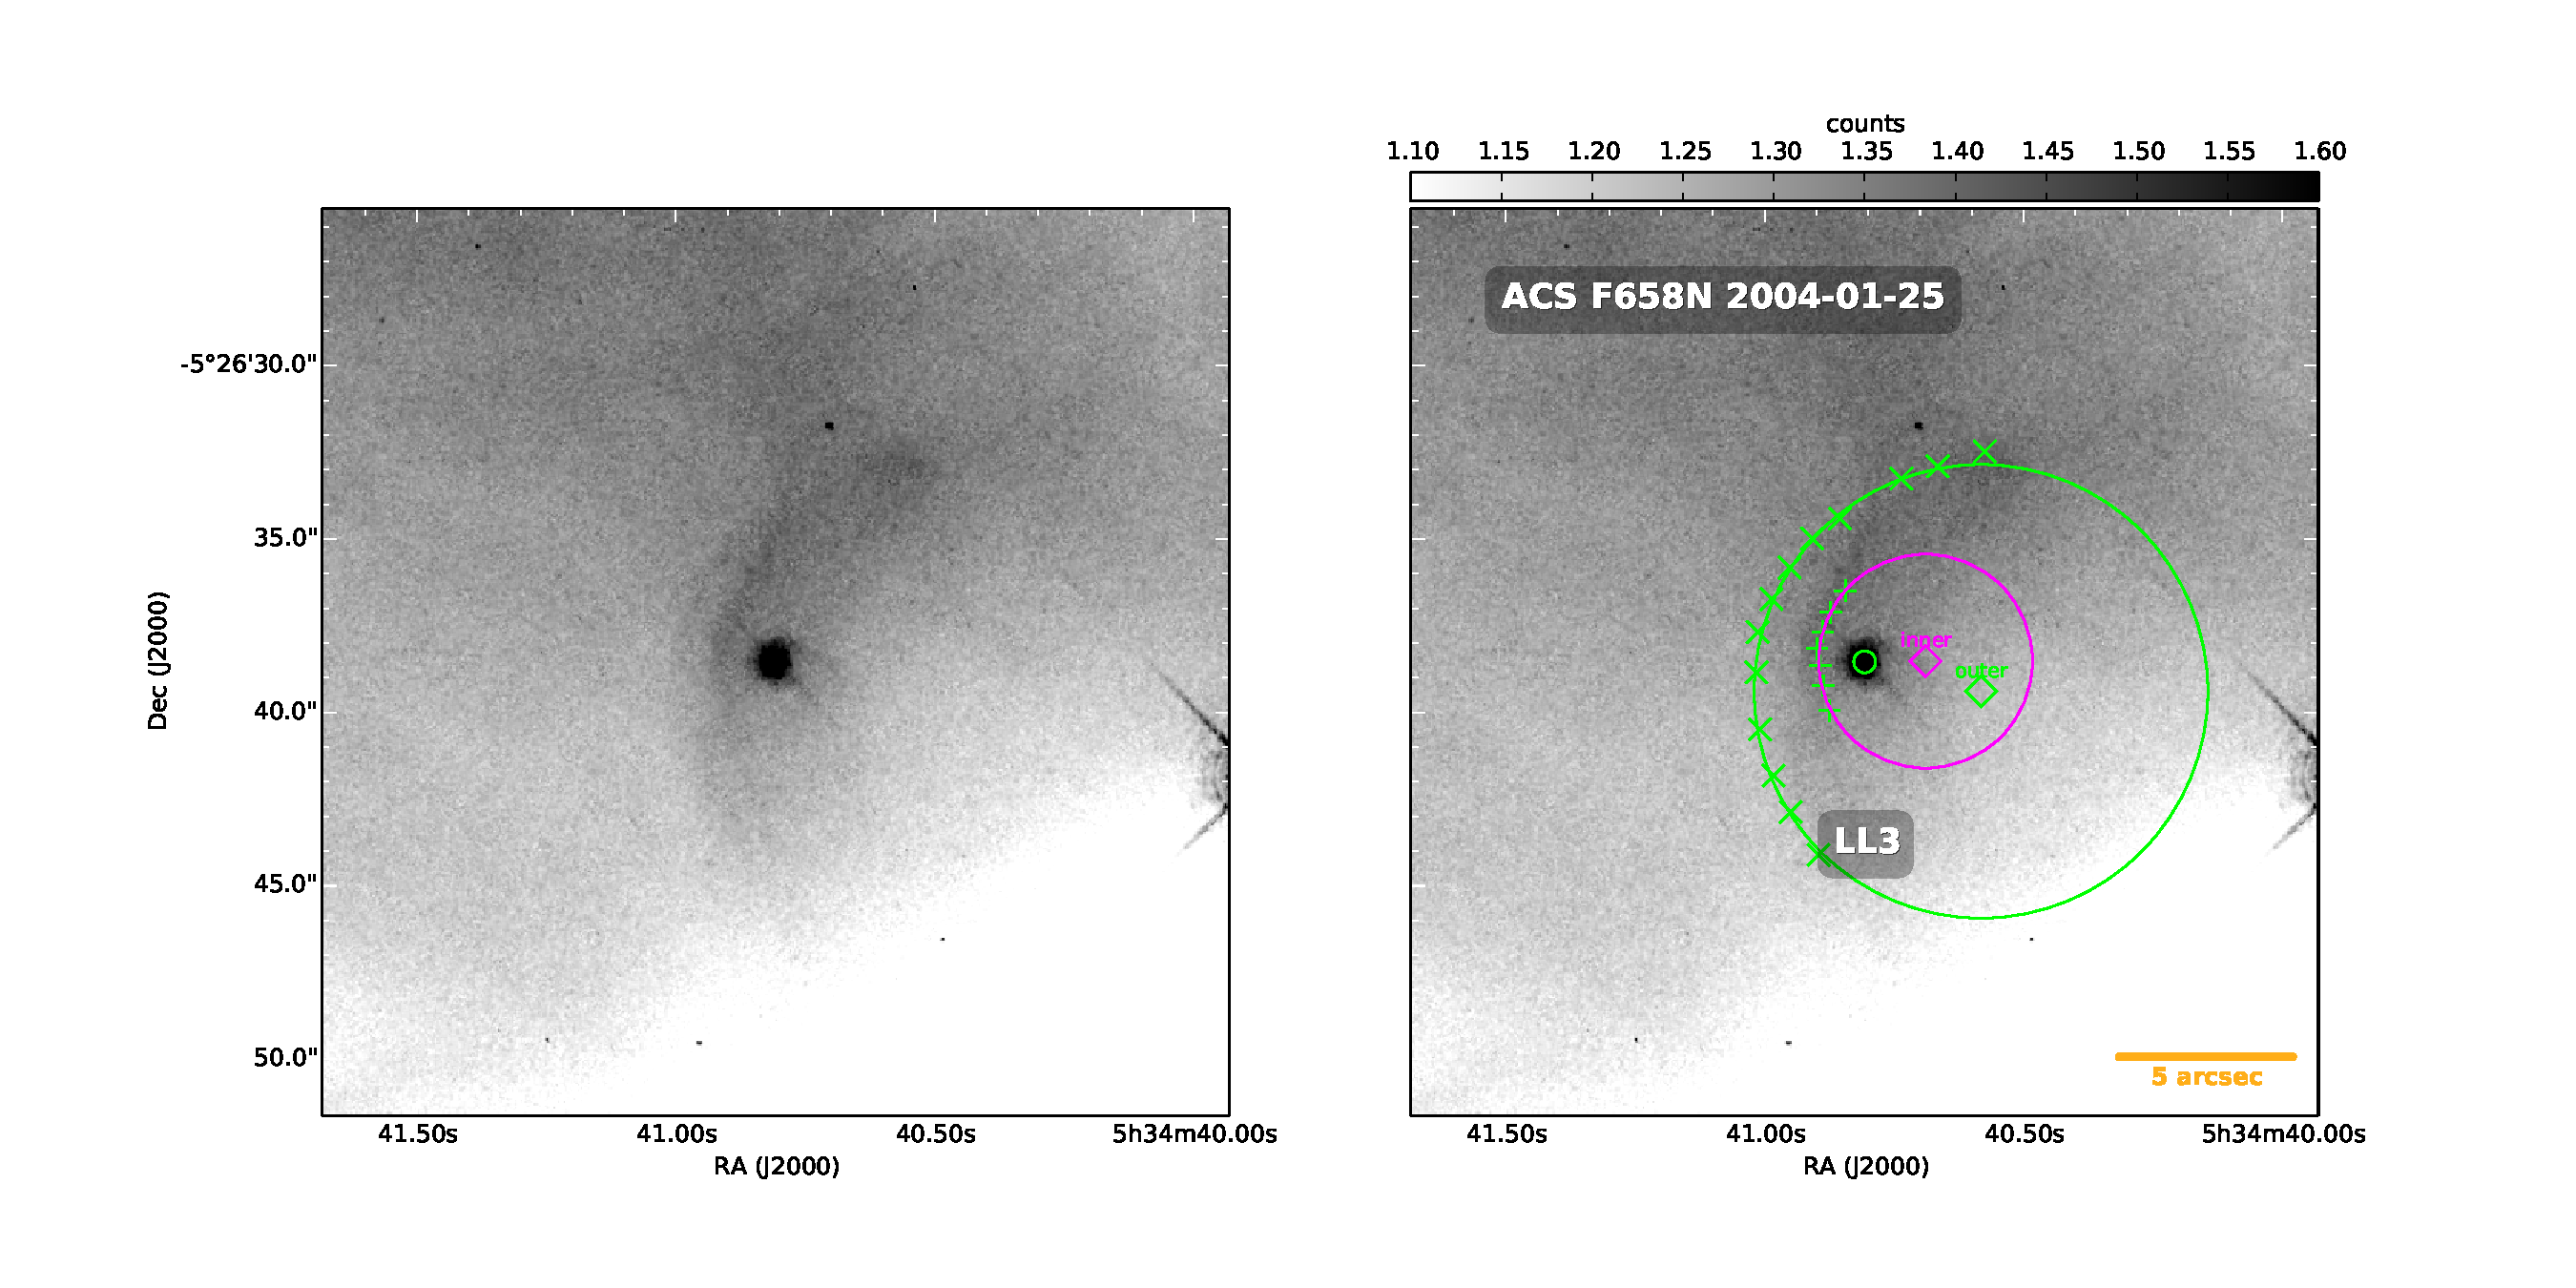
\includegraphics[width=0.5\linewidth]{./Figures/LL3-Bally_17-images}
  \end{tabular}
  \caption{}
  \label{fig:Luis-mosaic-2}
\end{figure}



\subsection{Mapa de Objetos}

A continuación mostramos el mapa de los objetos del catálogo de \citet{Gutierrez-Soto:2015a} dentro de la ONC.

\begin{figure}
  \centering
  \begin{tabular}{cc}
    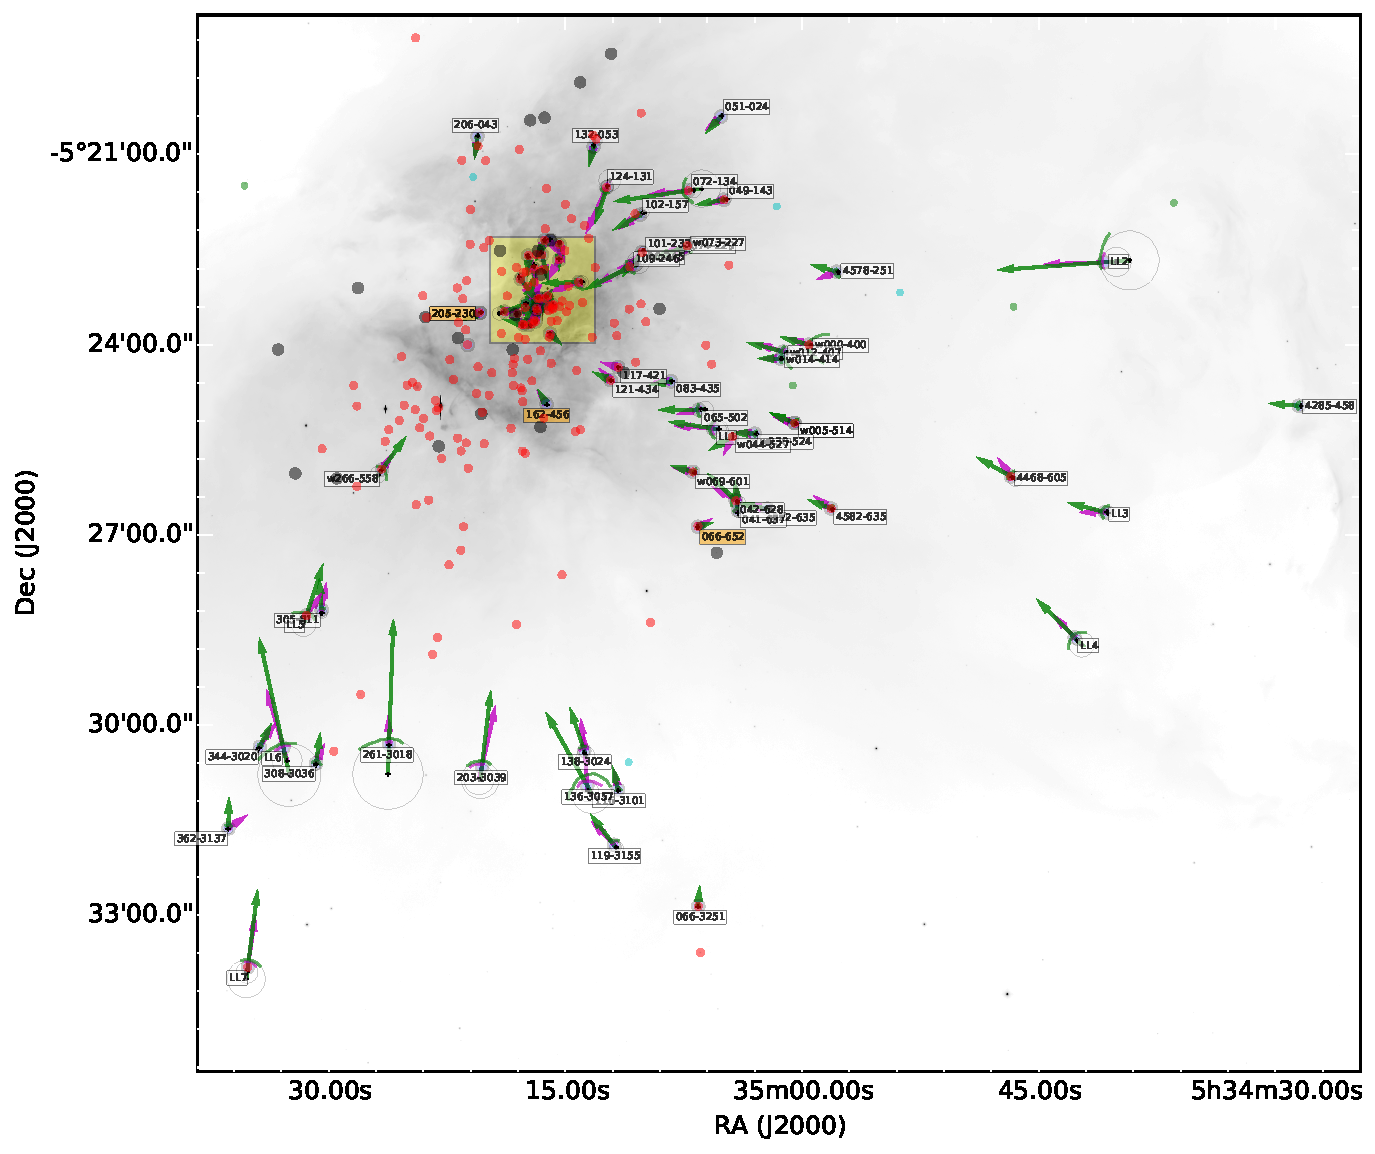
\includegraphics[width=0.5\linewidth]{./Figures/ll-pos-image-Luis} & 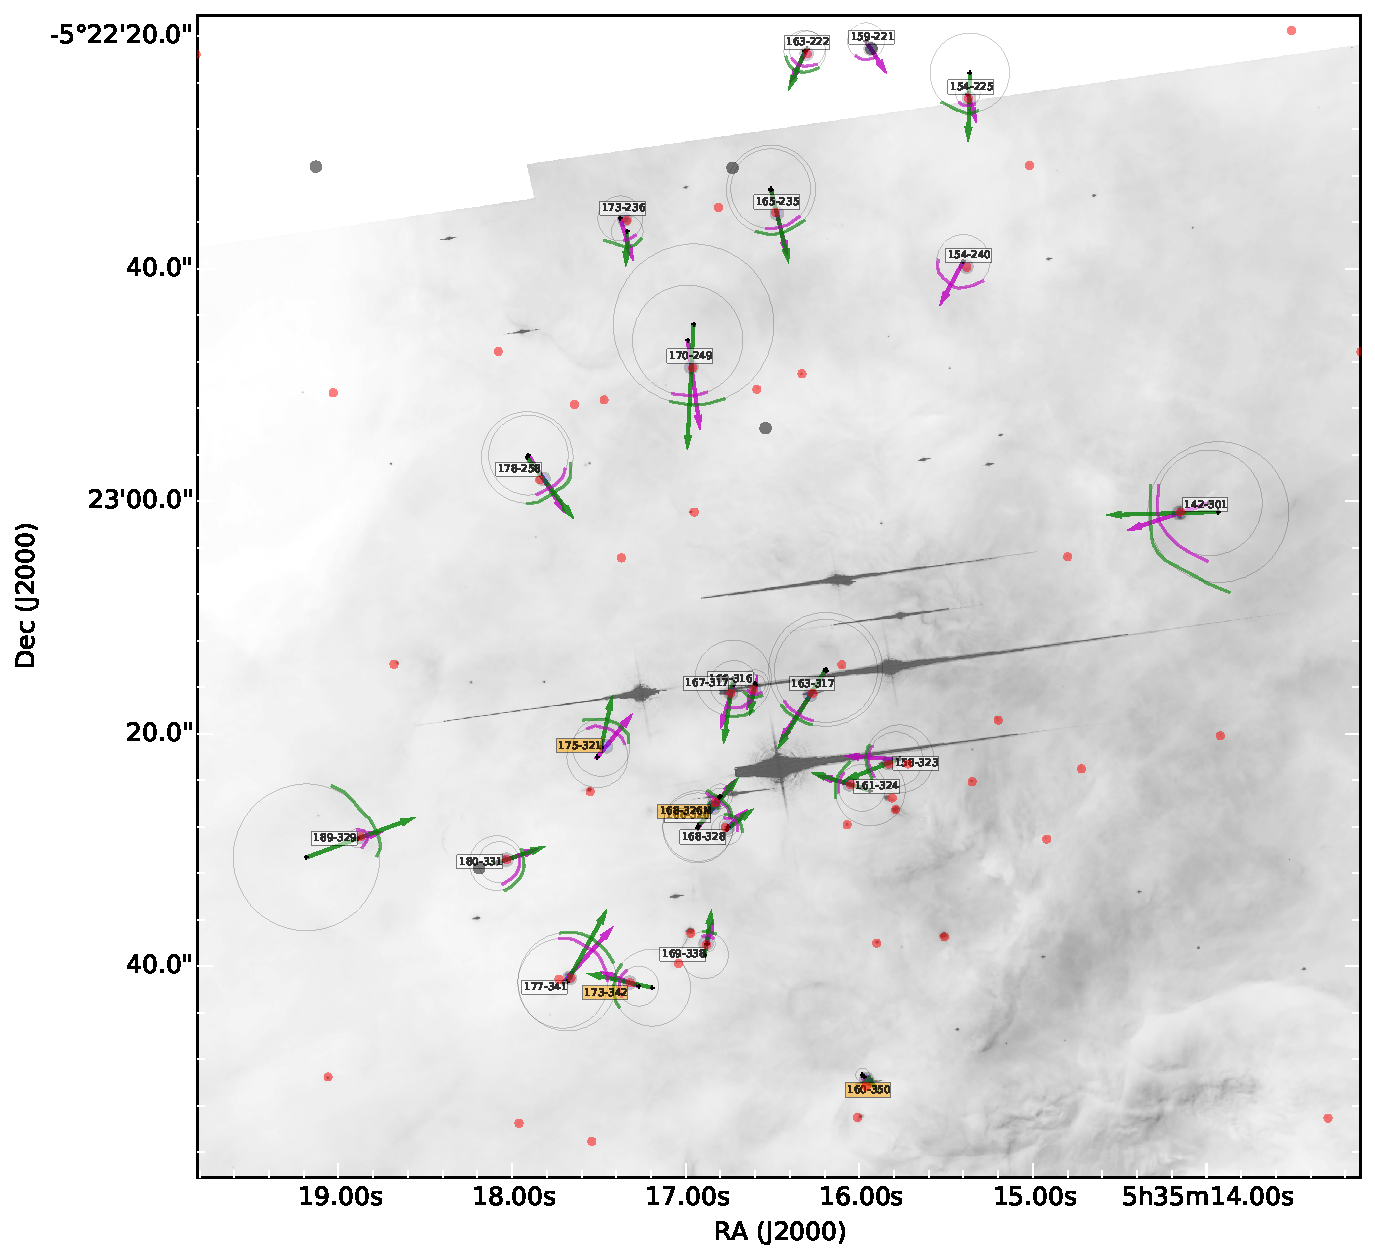
\includegraphics[width=0.46\linewidth]{./Figures/ll-pos-image-zoom-Luis}
  \end{tabular}
  \caption{Mapa de objetos del catálogo de \citet{Gutierrez-Soto:2015a} dentro de ONC. Las flechas de colores contienen la línea que une la posición del objeto central con el eje de curvatura de cada cáscara. Los puntos rojos representan objetos que no tienen un choque de proa visible. La zona marcada con el cuadrado amarillo se encuentra amplificada en el pánel derecho.}
  \label{fig:orion-map-LL}
\end{figure}


\section{Estrellas ``Errantes''}

Otro tipo de choques de proa estelares ocurren cuando los vientos de estrellas \textit{errantes} (runaway stars), usualmente de tipos espectrales OB, con velocidades de $ >\SI{30}{km.s^{-1}}$ interactúan con el medio interestelar \citep{Kobulnicky:2016}. Estas estrellas adquieren estas velocidades cuando sufren encuentros dinámicos cercanos dentro del cúmulo donde se formaron o bien cuando forman parte de un sistema binario cerrado y uno de los miembros explota como supernova.

En la figura \ref{fig:runaway} se muestran algunos ejemplos típicos de choques de proa producidos por estrellas errantes. Los colores en cada imagen representan a la banda de \SI{24}{\mu.m} del Telescopio Espacial Spitzer, o bien la de \SI{22}{\mu.m} del catálogo WISE para el color rojo, para el color verde puede ser la banda de \SI{8}{\mu.m} de Spitzer o la de \SI{12}{\mu.m} de WISE, y al color azul le corresponde la banda de \SI{4.5}{\mu.m} de Spitzer o WISE y los objetos mostrados son, de arriba a abajo y de izquierda a derecha: $\zeta$\,Oph, AE Aur, HD136003, HD150898, HD155755 y HD143275, y por último, la flecha blanca indica la magnitud y dirección del movimiento propio de la estrella.

\begin{figure}
  \centering
  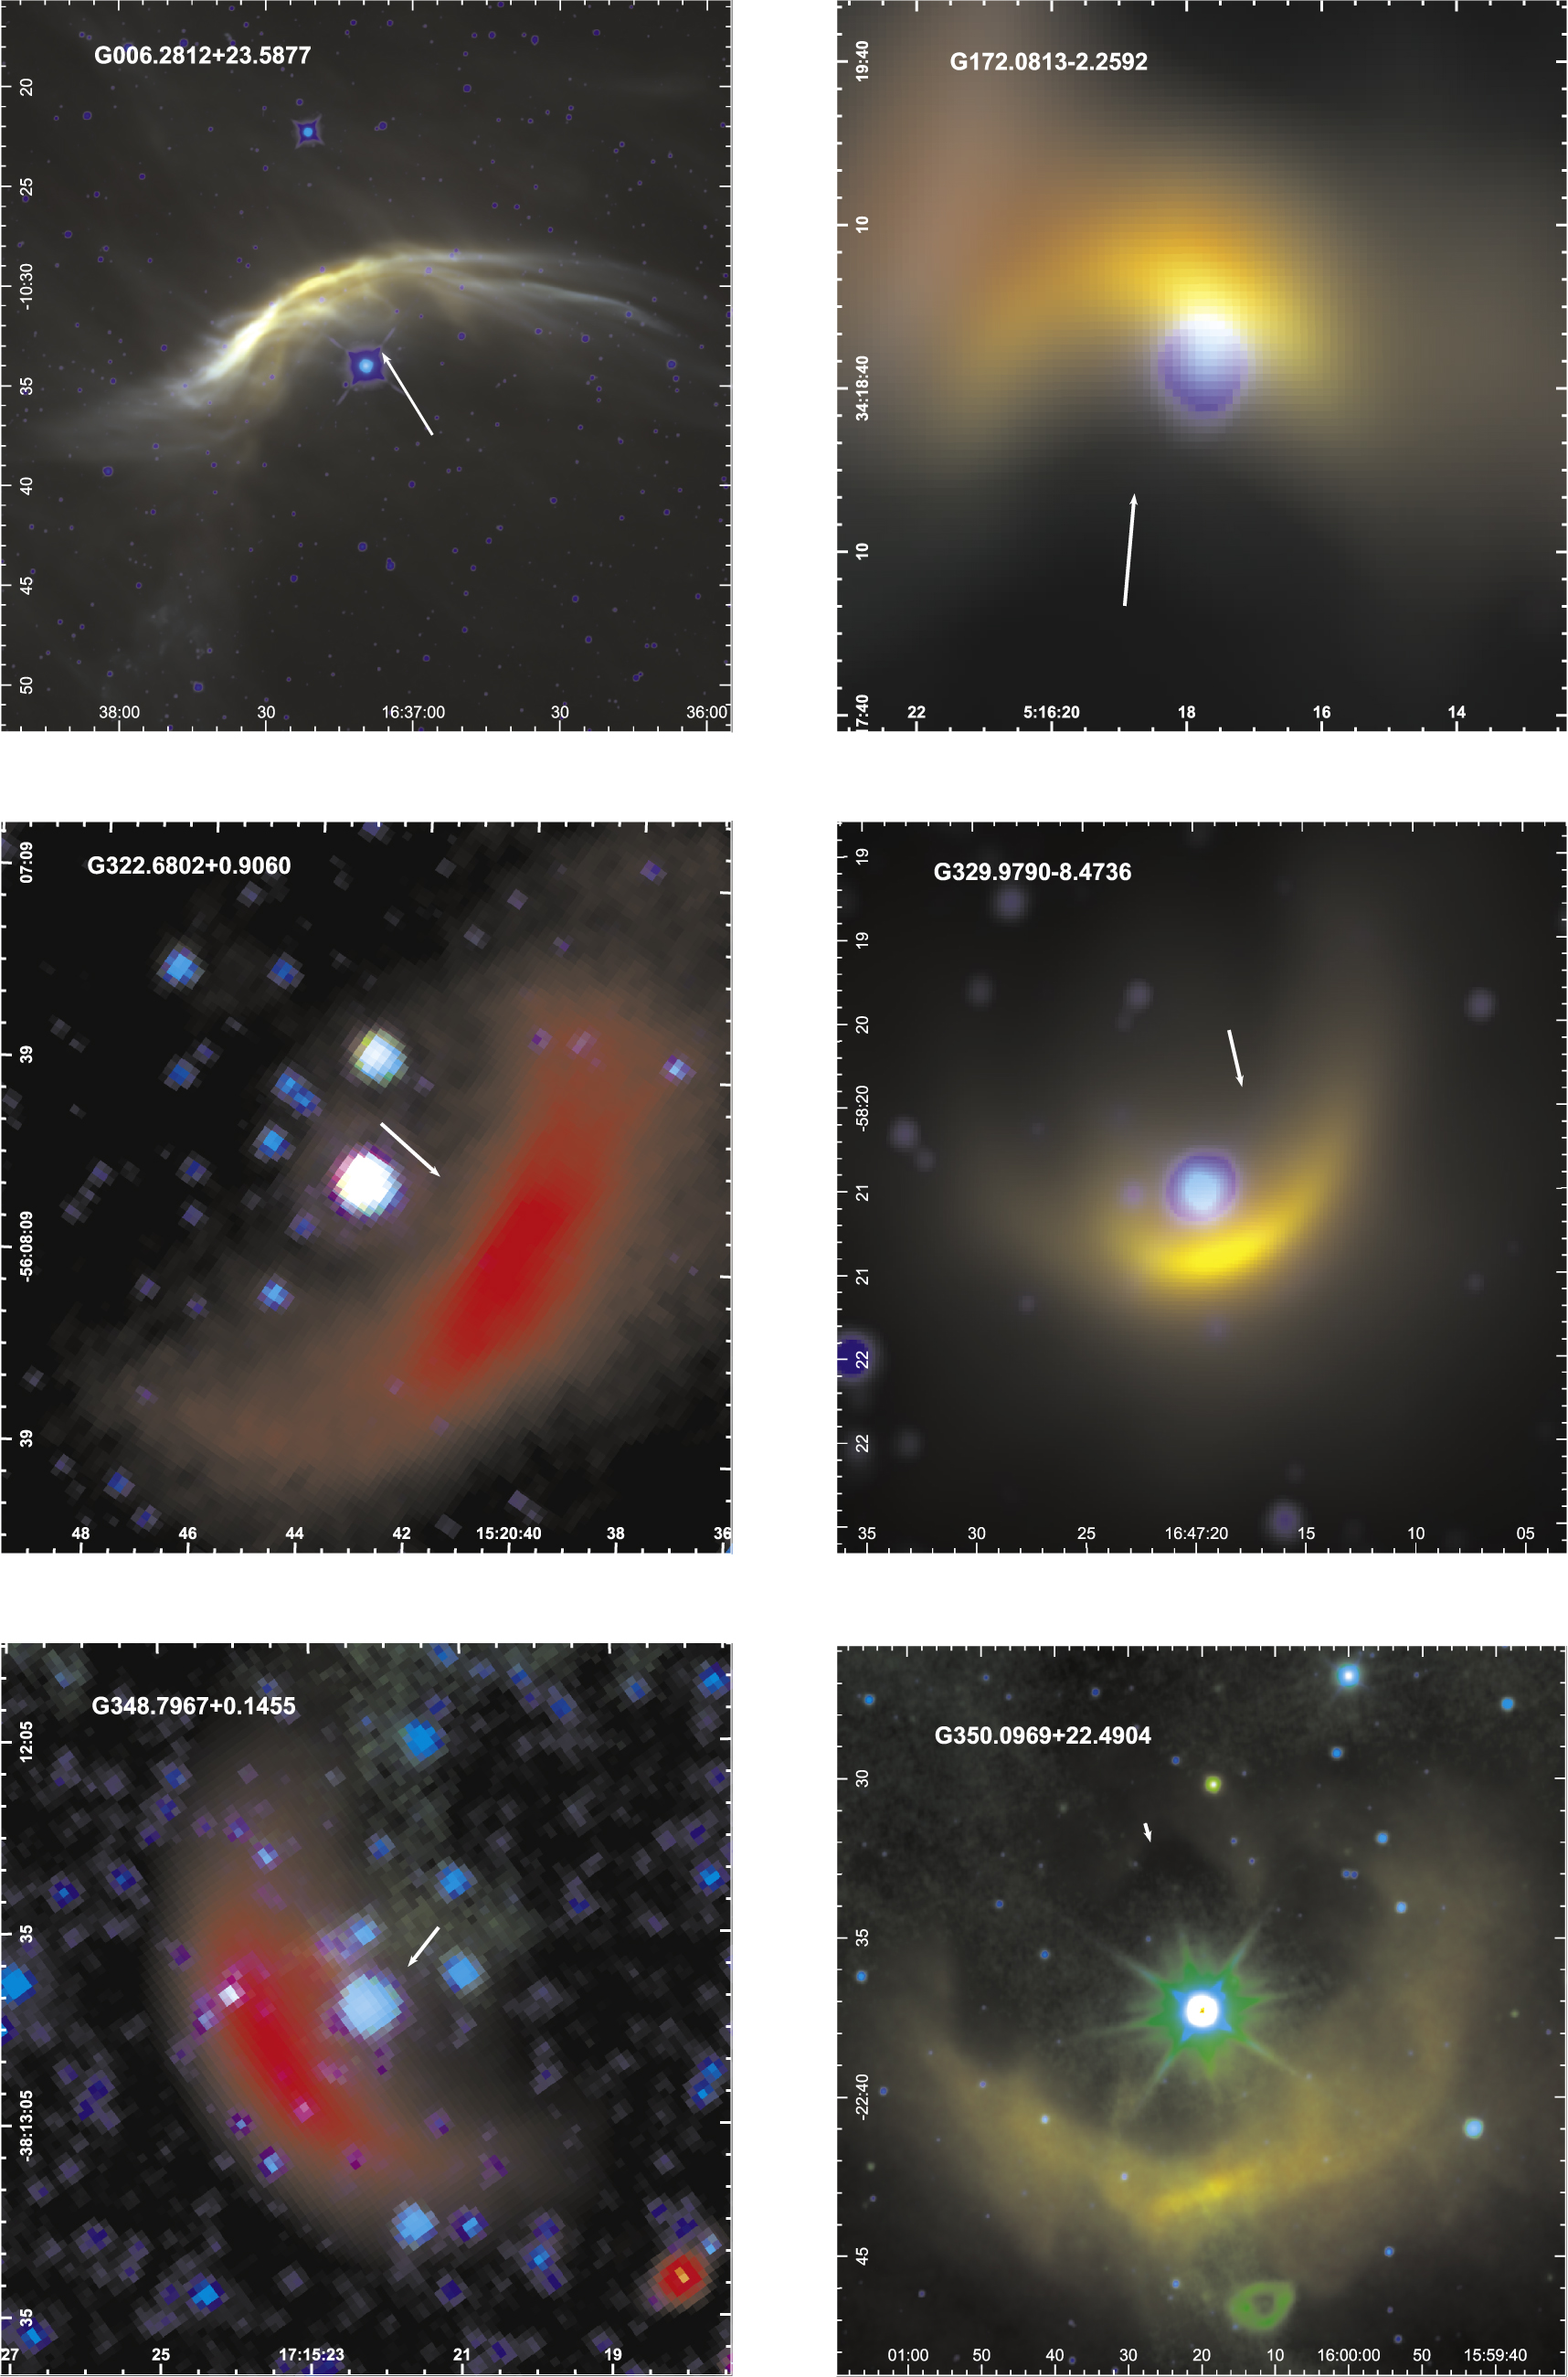
\includegraphics[width=0.7\linewidth]{./Figures/kobulnicky}
  \caption{Ejemplos de choques de proa en infrarrojo producidos por estrellas errantes, tomados por el telescopio espacial Spitzer o del catálogo WISE. Los colores representan las bandas de \SI{24}{\mu.m} de Spitzer o \SI{22}{\mu.m} de WISE (rojo), \SI{8}{\mu.m} de Spitzer o \SI{12}{\mu.m} de WISE (verde) y \SI{4.5}{\mu.m} de de Spitzer o WISE (azul). Los objetos mostrados son: $\zeta$\, Oph (G006.2812+23.5877; arriba izquierda), AE Aur (G172.0813-02.2592; arriba derecha), HD136003 (G322.6802+00.9060; centro izquierda), HD150898 (G329.9790-08.4736; centro derecha), HD155755 (G348.7967+00.1455; abajo izquierda) y HD143275 (G350.0969+22.4904; abajo derecha). La magnitud y dirección del movimiento propio se muestra con las flechas blancas \citep{Kobulnicky:2016}.}
  \label{fig:runaway}
\end{figure}

\section{Estrellas AGB y Supergigantes Rojas}

Otro tipo de choques de proa estelares se forma cuando estrellas en sus fases evolutivas finales, tales como estrellas AGB y supergigantes rojas pierden material a través de fuertes vientos que producen choques al interaccionar con el Medio Interestelar \citep{Cox:2012}.

En la figura  \ref{fig:fermata} se muestran ejemplos de estrellas AGB y supergigantes en infrarrojo lejano que forman parte del programa MESS (Mass-loss of Evolved StarS, \citet{Groenewegen:2011}) que utilizan el instrumento PACS (Photodetector Array Camera Spectrometer), donde se usan los filtros de \SI{70}{\mu.m} y \SI{160}{\mu.m}, y que muestran choques tipo ``fermata''. Otras formas que se observan son tipo ``ojos'', ``anillos'' e ``irregulares'' (ver tabla \ref{tab:morphology-AGB}).

\begin{figure}
  \centering
  \includegraphics[width=0.5\linewidth]{./Figures/Cox-fermata}
  \caption{Interacciones tipo ``fermata'' de los objetos R\,Scl, NML\,Tau, W\,Ori, W\,Pic y $\alpha$\,Ori tomadas con PACS en los filtros de \SI{70}{\mu.m} (izquierda) y \SI{160}{\mu.m} (derecha). La barra blanca mide 1' en la imagen, así como su respectivo tamaño físico. En todos los páneles el norte se ubica hacia arriba y el este a la izquierda. La línea negra indica la velocidad y dirección de la velocidad espacial de la estrella, adoptando una escala tal que \SI{1}{km.s} corresponde a 1'' en la imagen \citep{Cox:2012}. Nota adicional. R\,Scl tiene una cáscara esférica interna no visible en la imagen.}
  \label{fig:fermata}
\end{figure}

\begin{table}
  \centering
  \begin{tabular}{llc}
    \toprule
    Clase & Descripción & Forma \\
    \midrule
    I & Fermata & 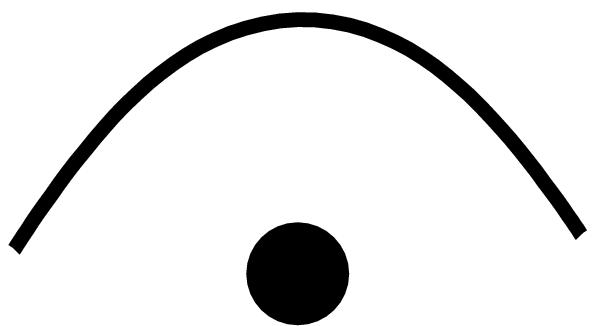
\includegraphics[scale=0.03]{./Figures/fermata} \\
    II & Ojos   & 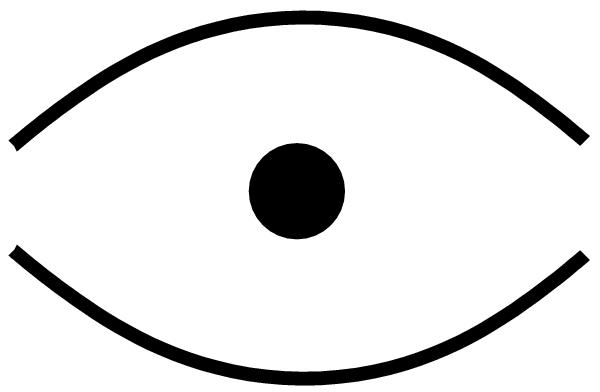
\includegraphics[scale=0.03]{./Figures/eyes} \\
    III & Anillos & 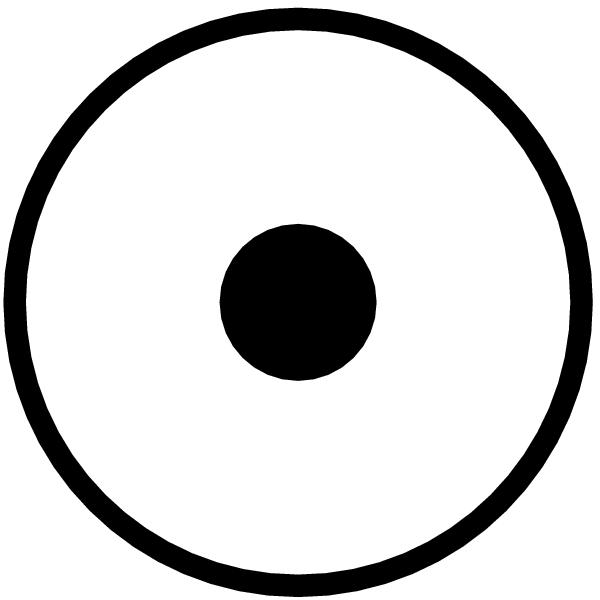
\includegraphics[scale=0.02]{./Figures/ring} \\
    IV & Irregulares & \\
    \bottomrule
  \end{tabular}
  \caption{Clasificación morfológica de choques de proa estelares de estrellas AGB y supergigantes \citep{Cox:2012}.}
  \label{tab:morphology-AGB}
\end{table}


%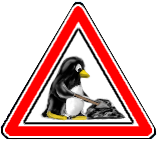
\includegraphics[width=0.1\linewidth]{./Figures/tux-development}

\chapter{Conceptos fundamentales}
\label{sec:Modelo-generico}
Para este trabajo consideramos en general dos modelos de interacción de vientos:
\begin{itemize}
\item Una fuente localizada en el origen que emite un viento esférico que puede ser isotrópico o anisotrópico (figura \ref{fig:isotropic-aniso}) no acelerado que interactúa con el viento esférico isotrópico de otra fuente que se encuentra a una distancia $D$ de la primera (figura \ref{fig:crw-esquema}). A los choques de proa resultantes se conocen como ``Cantoides'' y ``Ancantoides'', respectivamente.
\item Una fuente localizada en el origen que emite un viento esférico isotrópico no acelerado que interactúa con un viento plano paralelo no acelerado y densidad constante (figura \ref{fig:crw-esquema}b). Los choques resultantes en este caso se conocen como ``Wilkinoides''.
\end{itemize}
Para caracterizar al choque de proa utilizaremos coordenadas esféricas, siguiendo la simetría del viento interior. La forma del choque de proa medido a partir del origen es $R(\theta, \phi)$, donde $\theta$ y $\phi$ son el ángulo polar y azimutal, respectivamente. Asumiendo simetría cilíndrica en el sistema, esta función se simplifica a $R(\theta)$.
\begin{figure}
  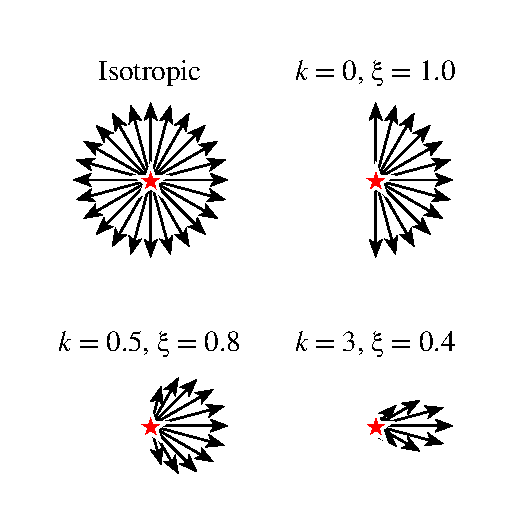
\includegraphics[width=0.5\linewidth]{./Figures/anisotropic-arrows}
  \caption{Representación esquemática de vientos con diferentes anisotropías: Arriba izquierda: Viento isotrópico esférico. Arriba derecha: viento isotrópico hemisférico. Abajo: Vientos anisotrópicos donde el parámetro $k$ indica el grado de anisotropía (ver capítulo \ref{chap:hipersonica})}
    \label{fig:isotropic-aniso}
\end{figure}
\begin{figure}
  \begin{tabular}{lr}
    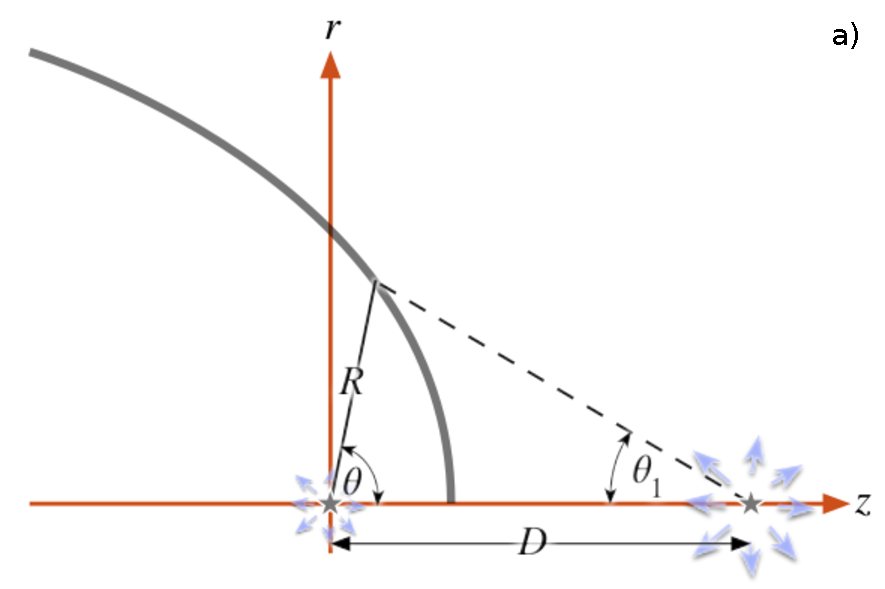
\includegraphics[width=0.45\linewidth]{./Figures/bowshock-crw-variables} &
    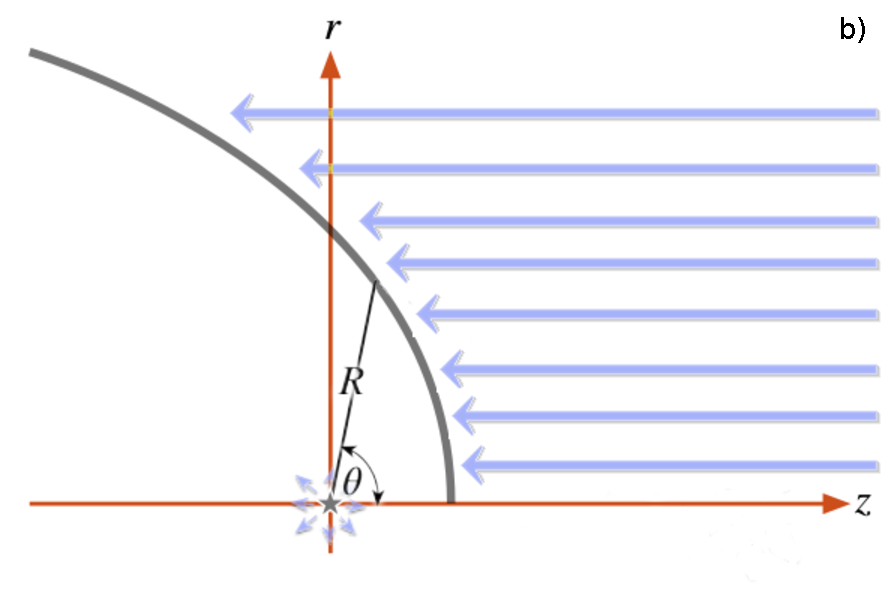
\includegraphics[width=0.45\linewidth]{./Figures/wilkinoid}
  \end{tabular}
  \caption{Izquierda: Representación esquemática del problema de interacción de dos vientos esféricos: Dos fuentes separadas por una distancia $D$ emiten un viento radial que forma un choque de proa a una distancia $R$ del origen. El sistema tiene geometría cilíndrica siendo el eje $z$ el eje de simetría. La forma del choque es función únicamente del ángulo polar $\theta$, medido a partir del origen. Otro ángulo que es de utilidad es $\theta_1$, que corresponde al ángulo polar medido a partir de la posición de la otra fuente. Cuando el viento interior tiene densidad constante y es esférico, denominamos al choque resultante como ``cantoide'', mientras que si su densidad sigue una ley de potencias de $\cos\theta$, siguiendo la ecuación (\ref{eq:Ancantoid-density}) del capítulo \ref{chap:hipersonica}, será un choque ``ancantoide''. Derecha: Representación esquemática de la interacción de un choque esférico e isotrópico con una corriente plano--paralela de densidad y velocidad constantes. El choque resultante es en este caso de tipo ``wilkinoide''.}
    \label{fig:crw-esquema}
\end{figure}

\section{Parámetros Fundamentales}

El valor mínimo de $R(\theta)$, bajo las condiciones ya mencionadas, ocurre en el ápex $(\theta=0)$, y lo denotamos como $R_0$. Bajo la condición de estado estacionario, la condición de equilibrio de presión ram entre ambos vientos implica que:

\begin{align}
  \frac{R_0}{D} = \frac{\beta^{1/2}}{1 + \beta^{1/2}}
\end{align}

Donde $\beta$ es la tasa de momentos entre los vientos en interacción. Si los dos vientos son isotrópicos, donde la tasa de pérdida de masa del viento interior es $\dot{M}_w$ y su velocidad terminal es $v_w$ y para el viento exterior estas cantidades son $\dot{M}_{w1}$ y $v_{w1}$, entonces la tasa de momentos es:

\begin{align}
  \beta = \frac{\dot{M}_w v_w}{\dot{M}_{w1} v_{w1}} \label{eq:beta-def}
\end{align}

En el caso de que el viento exterior sea una corriente plano--paralela (tipo wilkinoide, siguiendo a \citet{Wilkin:1996}), correspondería al caso en que $\beta\to 0$, entonces $D$ deja de ser un parámetro relevante, ya que técnicamente $D\to\infty$.

En el caso de que el viento interior no sea isotrópico es tratado en el capítulo \ref{chap:hipersonica}.

\section{Planitud y ``Alatud''}
\label{sec:char-rad}

$R_0$ no indica la escala del choque de proa, pero para caracterizar su forma utilizamos parámetros adicionales, mostrados en la figura \ref{fig:char-radii}. El radio perpendicular $R_{90}$ se obtiene evaluando la función $R(\theta)$ en $\theta=\pi/2$, mientras $R_c$ es el radio de curvatura medido en la posición del ápex, que en coordenadas cilíndricas se calcula como sigue (ver apéndice \ref{app:math-curvature-radius}):

\begin{align}
  R_c = \frac{R^2_0}{R_0 - R_{\theta\theta, 0}} \label{eq:generic-Rc}
\end{align}

donde $R_{\theta\theta, 0}\equiv \frac{d^2R}{d\theta^2}$ evaluado en $\theta = 0$.

Una forma simple de obtener el radio de curvatura es haciendo una expansión Taylor para la función $R(\theta)$ como sigue:

\begin{align}
  R(\theta) \simeq R_0 + \frac{1}{2}R_{\theta\theta, 0}\theta^2 + \mathcal{O}(\theta^4)
\end{align}
y hacer un ajuste polinomial a $R(\theta)$ para $|\theta| < \Delta\theta$ y determinar $R_0$ y $R_{\theta\theta, 0}$ de los primeros coeficientes del ajuste, y posteriormente $R_c$ a partir de la ecuación \ref{eq:generic-Rc}. $\Delta\theta$ es el rango del ángulo polar dentro del cual se puede hacer el ajuste. $\Delta\theta = 30^\circ$ es una buena opción.
%Las cantidades medibles que nos ayudan a caracterizar un choque de proa las llamamos ``Radios característicos'' (ilustrados en la figura \ref{fig:char-radii}):
%\begin{itemize}
%\item Radio en dirección perpendicular al ápex. Denotado como $R_{90}$
%\item Radio de curvatura en el ápex. Denotado como $R_c$. En el apéndice \ref{app:math-curvature-radius} se muestra el procedimiento para obtener este radio para una curva genérica continua y derivable.
%\end{itemize}

\begin{figure}
  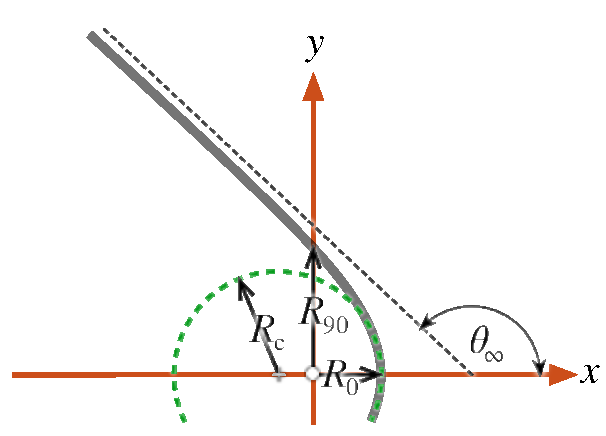
\includegraphics[width=0.5\linewidth]{./Figures/characteristic-radii}
  \caption{Representación esquemática de los radios característicos de un choque de proa}
  \label{fig:char-radii}
\end{figure}
Un último parámetro es el ángulo asintótico de apertura de las alas, denotado como $\theta_\infty$. Sin embargo, esta medida solo aplica para choques cuyas alas son asintóticamente cónicas, y aún para éstos en la mayoría de los casos es dificil de medirlo debido a que el ángulo polar $\theta$ tiende al valor asintótico muy lentamente y además la emisión de las alas es bastante débil. Por otro lado, los radios característicos $(R_0, R_c, R_{90})$ son medibles observacionalmente en la mayoría de los casos. A partir de éstos, podemos determinar dos parámetros adimensionales llamados ``planitud'' y ``alatud''. El primero de éstos es una medida de qué tan plano es el choque de proa en la nariz o ``apex'', y lo denotamos con la letra griega $\Pi$, mientras que el segundo es una medida de qué tanto se abren las alas del choque de proa, y lo denotamos con la letra griega $\Lambda$. Ambos parámetros se definen a continuación:

\begin{align}
  \Pi \equiv \frac{R_c}{R_0} \label{eq:planitude}\\
  \Lambda \equiv \frac{R_{90}}{R_0} \label{eq:alatude}
\end{align}

\section{Cuádricas de Revolución}
\label{sec:quadrics}
\newcommand\Sin{\ensuremath{\mathcal{S}}}
\newcommand\Cos{\ensuremath{\mathcal{C}}}
\newcommand\Cot{\ensuremath{\mathcal{T}}}
\newcommand\Q{\ensuremath{\mathcal{Q}}}
\newcommand\fQi{\ensuremath{f_{\scriptscriptstyle \Q, i}}}
En el caso general es difícil encontrar la forma aparente para un choque de proa siguiendo el formalismo desarrollado en la sección anterior, por lo que optamos por aproximar la forma éstos con una de las superficies más simples: las \textit{cuádricas de revolución}, que son superficies de revolución de las curvas cónicas. Dado el modelo general descrito en la \S \ref{sec:Modelo-generico}, haremos algunas restricciones para las superficies cuádricas que utilizaremos en este trabajo:
\begin{itemize}
  \item El eje focal se encuentra alineado con el eje $x$
  \item La posición del foco de la superficie cuádrica no necesariamente coincide con la posición de la fuente
  \item En el caso de las hipérbolas, solo tomamos una de las ramas de ésta.
\end{itemize}
Implementando dichas restricciones, utilizamos la representación paramétrica de las curvas cónicas en términos de un parámetro adimensional denotado con la letra $t$:
\begin{align}
  x &= x_0 + \sigma a\Cos(t) \\
  y &= b\Sin(t) 
\end{align}
Donde:
\begin{align}
  \Cos(t), \Sin(t) &=\left\lbrace
  \begin{array}{lr}
    \cos{t}, \sin t & \mathrm{elipses}\\
    \cosh{t}, \sinh{t} & \mathrm{hipérbolas}       
  \end{array}\right. \\
  \sigma &= \left\lbrace
  \begin{array}{lr}
    +1 & \mathrm{elipses} \\
    -1 & \mathrm{hipérbolas}
  \end{array}\right. \\
  x_0 &= R_0 -\sigma a \label{eq:x0} 
\end{align}
Donde $a$ y $b$ representan la longitud de los semi-ejes de la cónica en cuestión (Figura \ref{fig:conics}). $x_0$ representa la distancia entre el centro de la cónica y el origen. 

La forma polar del choque de proa $R(\theta)$ viene dada por:

\begin{align}
  \tan\theta &= \frac{b\Sin(t)}{a\Cos(t) + x_0} \label{eq:t-th-conversion} \\
  R &= \left(\left(a\Cos(t) + x_0\right)^2 + b^2\Sin^2(t)\right)^{1/2} 
\end{align}
El tipo de cónica lo podemos caracterizar mediante el parámetro $\Q$, donde:
\begin{align}
  \Q \equiv \sigma\frac{b^2}{a^2} \label{eq:conic-parameter-a-b}
\end{align}
Para las superficies abiertas (hiperboloides) tenemos que $\Q < 0$, mientras que para las superficies cerradas tenemos que $\Q > 0$. Casos particulares son la esfera $\Q = 1$ y el paraboloide $\Q = 0$. De manera equivalente se puede definir el ángulo $\theta_Q$ como sigue:
\begin{align}
  \tan\theta_Q = \sigma \frac{b}{a} \label{eq:thc}
\end{align}
Este ángulo se relaciona con la excentricidad de las cónicas (y que sustituye a esta última en este trabajo) como se muestra a continuación:
\begin{align}
  \tan\theta_Q = \sigma\sqrt{\left|1-e^2\right|}
\end{align}
\begin{figure}
  \begin{tabular}{cc}
    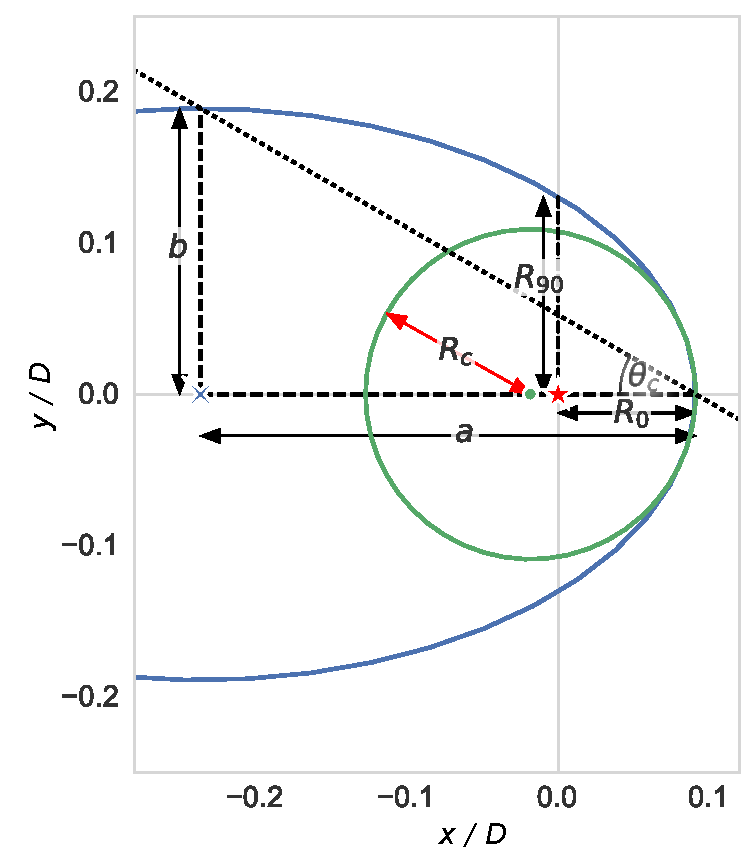
\includegraphics[width=0.4\linewidth]{./Figures/ellipse_edited} &
    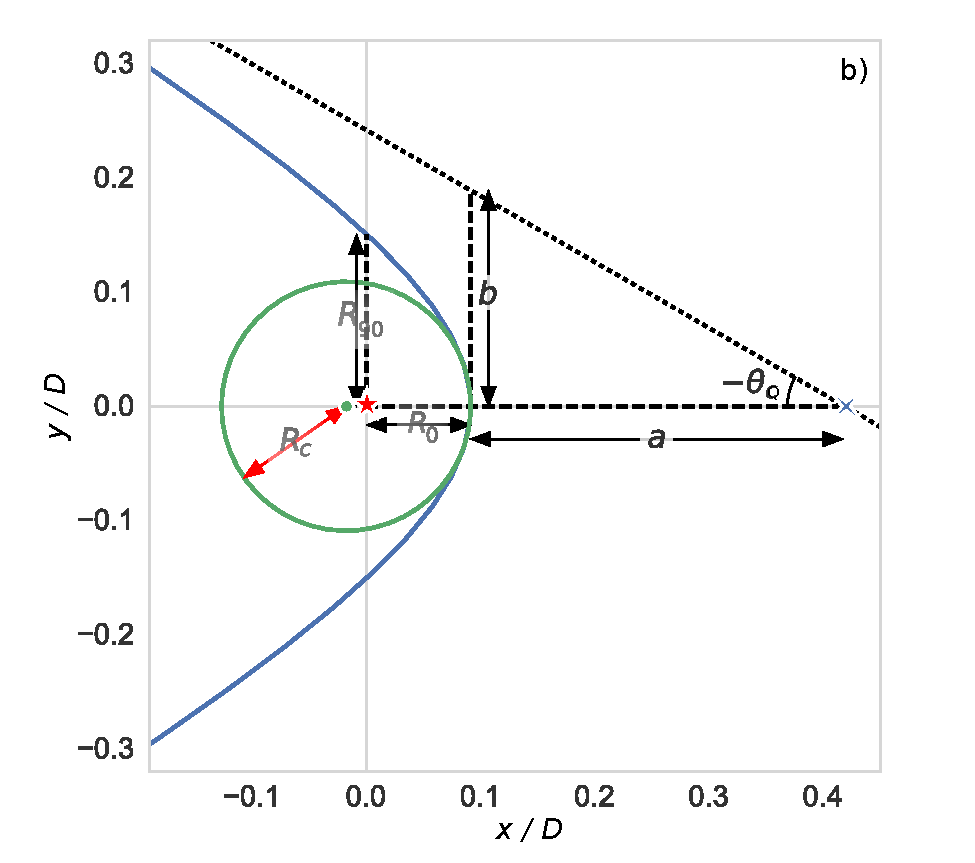
\includegraphics[width=0.5\linewidth]{./Figures/hyperbola_edited}
  \end{tabular}
  \caption{Representación esquemática de: Izquierda: Elipse. Y, derecha: Hipérbola. En ambos casos se ilustran los parámetros relevantes de éstas y los radios característicos}
  \label{fig:conics}
\end{figure}

\begin{figure}
  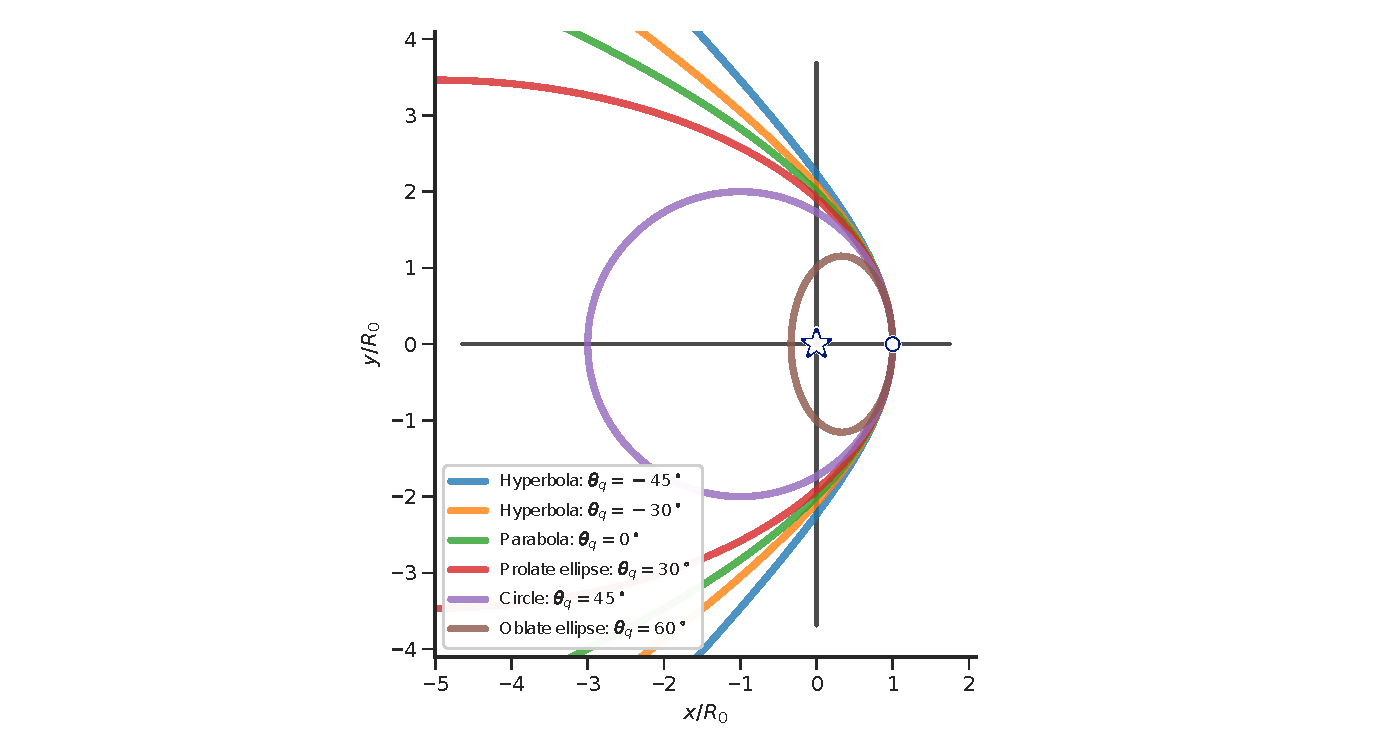
\includegraphics[width = 0.5\linewidth]{./Figures/conic1}
  \caption{Familia de curvas cónicas, donde el valor del parámetro $\theta_Q$ varía desde $\theta_Q < 0$ (hipérbolas) hasta $\theta_Q > 0$ (elipses). Casos especiales son $\theta_Q = 0$ (parábola) y $\theta_Q = 45^\circ$ (círculo). Este parámetro sustituye en este trabajo a la excentricidad.}
  \label{fig:conics-family}
\end{figure}
El set de parámetros $(a, x_0, \Q)$ es suficiente para caracterizar a nuestras cuádricas de revolución: $\Q$ nos indica el tipo de cónica, $a$ establece la escala y $x_0$ el desplazamiento del centro a lo largo del eje x. Sin embargo, para futuras aplicaciones tanto a modelos de interacción de vientos como a observaciones (capítulos \ref{chap:hipersonica} y \ref{chap:proplyds}) nos sería util hacer la caracterización mediante los parámetros $(R_0, \Pi, \Lambda)$ (ver \S \ref{sec:char-rad}). Las equivalencias entre los dos sets de parámetros los calculamos a continuación:
\begin{align} 
  R_c &= \frac{b^2}{a} = a|\Q|\label{eq:R-curv-conic}\\
  R^2_{90} &= b^2\sigma\left(1 - \frac{x^2_0}{a^2}\right) = \Q\left(a^2 - x^2_0\right)\label{eq:R90-conic} 
\end{align}
Combinando las ecuaciones (\ref{eq:planitude}, \ref{eq:alatude}, \ref{eq:x0}, \ref{eq:conic-parameter-a-b}, \ref{eq:R-curv-conic}, \ref{eq:R90-conic}), obtenemos lo siguiente:

\begin{align}
  R_0 &= x_0 + \sigma a \label{eq:R0}\\
  \Pi &= \frac{a|\Q|}{x_0 + \sigma a} = \frac{a\Q}{\sigma\left(x_0 + \sigma a\right)} = \frac{a\Q}{\left(a + \sigma x_0\right)}\label{eq:quadric-planitude}\\
  \Lambda &= \left(\Q\frac{a-\sigma x_0}{a + \sigma x_0}\right)^{1/2}
\end{align}

De aquí podemos escribir el parámetro de las cuádricas $\Q$ en términos de la planitud y la alatud:

\begin{align}
  \Q = 2\Pi - \Lambda^2 \label{eq:quadric-parameter-pi-lambda}
\end{align}

Por tanto, el signo de $2\Pi - \Lambda^2$ determina si una cuádrica es esferoidal o hiperboloidal. En la figura \ref{fig:conics-family} mostramos como, para planitud constante, podemos tener una familia de cónicas variando únicamente la alatud, y por consiguiente, el parámetro $\Q$.

\section{Proyección en el Plano del Cielo}
\label{sec:projection}

Para un choque de proa que es la vez geométricamente delgado y ópticamente delgado, únicamente se observa el borde de éste por
abrillantamiento al limbo, por lo tanto, su orientación respecto a la línea de visión modifica su forma respecto a la forma real del
choque. Para ello, rotamos el sistema de referencia del choque de proa en coordenadas cartesianas, denotado por $(x, y, z)$, por un ángulo que llamamos \textit{inclinación}, denotado por $i$, en el plano $xz$. La inclinación está definida de modo que cuando $i=0^\circ$ el eje de simetría del choque es perpendicular a la línea de visión, es decir, lo observamos ``de canto''. Y cuando $i = 90^\circ$ el eje desimetría es paralelo a la línea de visión, es decir, que lo observamos ``de frente''. De este modo la transformación entre el sistema de refencia del choque y el sistema de referencia del plano del cielo, denotado por $(x', y', z')$ queda como sigue:
\begin{align}
  \left(
  \begin{array}{c}
    x' \\ y' \\ z'
  \end{array}
  \right) = \mathbf{A}_y(i)
  \left(
  \begin{array}{c}
    x \\ y \\ z
  \end{array}
  \right) =
  \left(
  \begin{array}{c}
    x\cos i - z\sin i \\ y' \\ z\cos i + x\sin i
  \end{array}
  \right)
  \label{eq:rotation}
\end{align}

Donde $\mathbf{A}_y(i)$ está definida en el apéndice \ref{app:matrix}
Por otro lado, la forma tridimensional del choque de proa viene dado por:
\begin{align}
  \left(
  \begin{array}{c}
    x \\ y \\ z
  \end{array}
  \right) &=
            R(\theta)\left(
            \begin{array}{c}
              \cos\theta \\
              \sin\theta\cos\phi \\
              \sin\theta\sin\phi
            \end{array}
            \right)
\end{align}
La relación entre ambos sistemas de referencia se ilustra en la figura \ref{fig:reference}.
\begin{figure}
  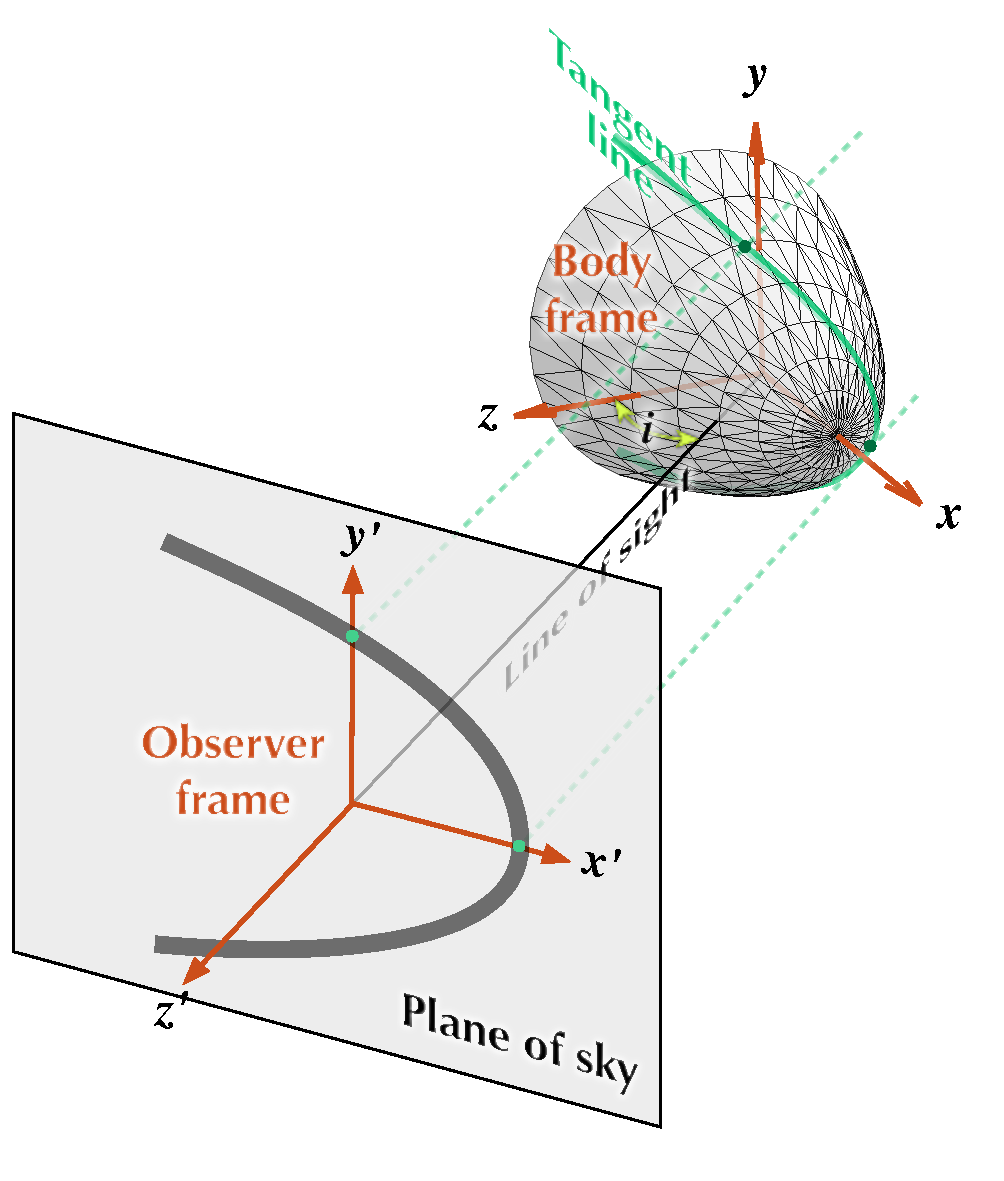
\includegraphics[width=0.5\linewidth]{./Figures/projection-pos}
  \caption{Sistema de referencia del choque vs sistema de referencia del plano del cielo. Los ejes $x'$ y $y'$ se encuentran en el plano del cielo, mientras el eje $z'$ es paralelo a la línea de visión. Solo la región del choque cuya tangente sea paralela a la línea de visión será visible por abrillantamiento al limbo.}
  \label{fig:reference}
\end{figure}

\subsection{Vectores normal y tangente a la superficie}

Si definimos los vectores $\hat{n}$ y $\hat{t}$, como los vectores normal y tangente a la superficie, respectivamente para $\phi$ constante. En el caso $\phi = 0$ (figura \ref{fig:unit-vec}), ambos vectores se encuentran en el plano $xy$ y es fácil mostrar que:
\begin{align}
  \hat{t}_0 =
  \left(
  \begin{array}{c}
    -\cos\alpha \\
    \sin\alpha \\
    0
  \end{array}
  \right)
  \quad \mathrm{y} \quad
  \hat{n}_0 =
  \left(
  \begin{array}{c}
    \sin\alpha \\
    \cos\alpha \\
    0
  \end{array}
  \right)
  \label{eq:unit-vec}
\end{align}
Donde:
\begin{align}
  \tan\alpha = -\frac{dy}{dx} = \frac{1+\omega\tan\theta}{\tan\theta-\omega}
\end{align}
y:
\begin{align}
  \omega(\theta) = -\frac{1}{R}\frac{dR}{d\theta} 
\end{align}
Para $\phi \neq 0$, basta con hacer una rotación de las ecuaciones (\ref{eq:unit-vec}) alrededor del eje $x$ utilizando la matriz de rotación $\mathbf{A}_x(\phi)$ (ecuación ):

\begin{align}
  \hat{n} &= \mathbf{A}_x(\phi)\hat{n}_0 =
 \left(
  \begin{array}{c}
    \sin\alpha \\
    \cos\alpha\cos\phi \\
    \cos\alpha\sin\phi
  \end{array}
  \right) \quad
    \hat{t} &= \mathbf{A}_x(\phi)\hat{t}_0 =
 \left(
  \begin{array}{c}
    -\cos\alpha \\
    \sin\alpha\cos\phi \\
    \sin\alpha\sin\phi
  \end{array}
  \right)
\end{align}

\begin{figure}
  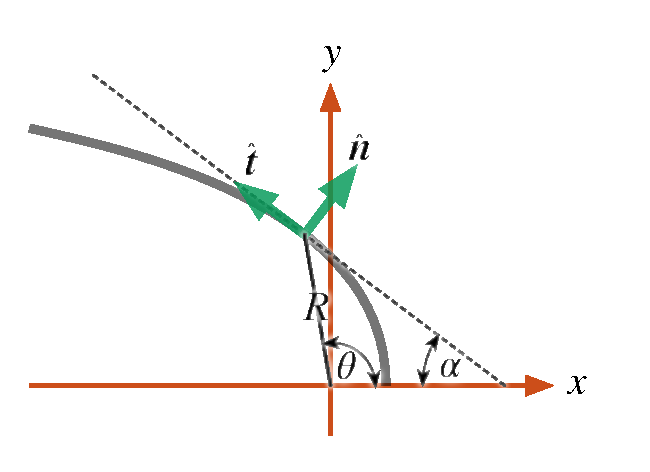
\includegraphics[width=0.6\linewidth]{./Figures/bowshock-unit-vectors}
  \caption{Vectores unitarios normal y tangente a la superficie $R(\theta)$
    en un plano de azimuth $\phi$ constante.}
    \label{fig:unit-vec}
\end{figure}

\subsection{Línea tangente}
\label{sec:tangent-line}
Debido a que el choque es ópticamente delgado y geométricamente delgado, solo la región del choque cuya tangente sea paralela a la
línea de visión seré visible. Esto corresponde a una curva que denominamos \textit{línea tangente}, que debe cumplir con la siguiente
condición:
\begin{align}
  \hat{n}\boldsymbol{\cdot} \hat{z}' = 0
\end{align}
Denotamos como $\phi_T$ al ángulo azimutal que cumple la condición anterior para una inclinación dada, en función del ángulo polar $\theta$:
\begin{align}
  \sin\phi_T = -\tan i\tan\alpha = \tan i\frac{1+\omega\tan\theta}{\omega-\tan\theta}
  \label{eq:phi-tan}
\end{align}
De esta manera, la forma de la línea tangente del choque de proa, a la que llamamos \textit{forma proyectada} viene dada por:
\begin{align}
  \left(
  \begin{array}{c}
    x'_T \\
    y'_T \\
    z'_T
  \end{array}
  \right) =
  R(\theta)\left(
  \begin{array}{c}
    \cos\theta\cos i - \sin\theta\sin\phi_t\sin i \\
    \sin\theta\left(1-\sin^2\phi_T\right)^{1/2} \\
    \cos\theta\sin i + \sin\theta\sin\phi_T\cos i
  \end{array}
  \right) \label{eq:proj-shape}
\end{align}
En el caso general, $z'_T$ no es una función lineal de $x'_T$ y $y'_T$, por lo que la línea tangente no se encuentra en un plano. La forma aparente $(x'_T, y'_T)$  de la línea tangente también puede escribirse en coordenadas polares $(R', \theta')$, donde:
\begin{align}
  R'(\theta) = \left(x'^2_T + y'^2_T\right)^{1/2} \quad \mathrm{y} \quad \tan\theta' = \frac{y'_T}{x'_T}
  \label{eq:polar}
\end{align}
Es de notar a su vez que la ecuación (\ref{eq:phi-tan}) no tiene solución para valores arbitrarios de $\theta$ y de la inclinación, puesto que se requiere que $\left|\sin\phi_T\right| < 1$. Por tanto, la línea tangente solo existe para valores de $\theta$ tales que $\theta < \theta_0$ donde $\theta_0$ es el valor de $\theta$ en el eje de simetría de la línea tangente proyectada $(\theta'(\theta_0) = 0)$ y que se obtiene resolviendo la siguiente ecuación implícita:
\begin{align}
  \tan\theta_0 = \frac{|\tan i| + \omega(\theta_0)}{1 - \omega(\theta_0)|\tan i|}
  \label{eq:th-0}
\end{align}
Esto implica que si el choque de proa es suficientemente ``abierto'' $(\alpha > \alpha_{min})$, entonces para inclinaciones tales que
$|i| > 90^\circ - \alpha_{min}$ no existirá la línea tangente para ningún valor de $\theta$, es decir, el choque de proa se encontrará sufientemente ``de cara'' como para que ya no parezca un choque de proa para el observador.

\subsection{Planiud y Alatud proyectadas: caso general}

En orden de comparar la forma $R(\theta)$ con observaciones, es útil definir los radios característicos $R'_0$ y $R'_{90}$, donde $R'_0$ es el radio del eje de simetría aparente y $R'_{90}$ es el radio aparente en la dirección perpendicular a $R'_0$. Es decir
$R'_0 = x'_T(y'_t=0)$ y $R'_{90} = y'_t(x'_t = 0)$. Utilizando las ecuaciones (\ref{eq:phi-tan}) y (\ref{eq:proj-shape}) encontramos que:
\begin{align}
R'_0 = R(\theta_0)\cos(\theta_0 - |i|)\footnotemark
\label{eq:R0p}
\end{align}\footnotetext{Evaluando la ecuación (\ref{eq:phi-tan}) en $\theta=\theta_0$ con ayuda de la ecuación (\ref{eq:th-0}) encontramos que $\sin\phi_T(\theta_0) = -\frac{\tan i}{|\tan i|}$ por lo que al sustituir este resultado en la componente $x$ de la ecuación (\ref{eq:proj-shape}) encontramos que $R'_0 = R(\theta_0)\left(\cos\theta_0\cos i + \sin\theta_0\sin i\frac{\tan i}{|\tan i|\right)}$ que finalmente se reduce al resultado de la ecuación (\ref{eq:R0p})}
Donde $\theta_0$ es la solución de la ecuación (\ref{eq:th-0}), y
\begin{align}
  R'_{90} = R(\theta_{90})\sin\theta_{90}\left(1-\sin^2\phi_T(\theta_{90})\right)^{1/2}
  \label{eq:R90p}
\end{align}
donde $\theta_{90}$ es la solución de la siguiente ecuación implícita:
\begin{align}
  \cot\theta_{90} = \frac{1 - \left(1+\omega(\theta_{90})^2\sin^22i\right)^{1/2}}
  {2\omega(\theta_{90})\cos^2i}
  \label{eq:th90}
\end{align}

El radio de curvatura aparente se obtiene a partir de la ecuación (\ref{eq:generic-Rc}) pero en el sistema de referencia primado:

\begin{align}
  R'_c = \frac{R'^2_0}{R'_0 - R'_{\theta'\theta', 0}} \label{eq:Rc-prime}
\end{align}

\subsection{Aplicación a las Cuádricas de Revolución}
\label{sec:pi-lambda-quadric}
El objetivo de esta sección es obtener la forma proyectada de las cuádricas de revolución, puesto que son una aproximación buena y mucho más sencilla a la forma real de un choque de proa. Para esto es conveniente utilizar un sistema de referencia donde el origen se ubica en el centro de la sección cónica:

\begin{align}
  (X, Y, Z) = (x-x_0, y, z)
\end{align}

De esta manera, la forma de la cuádrica de revolución es:

\begin{align}
  X &= a\Cos(t) \\
  Y &= b\Sin(t)\cos\phi \\
  Z &= b\Sin(t)\sin\phi
\end{align}

Siguiendo el procedimiento mostrado en la \S \ref{sec:projection} calculamos el ángulo azimutal $\phi$ que cumple con el criterio de ser tangente a la línea de visión: 

\begin{align}
  \sin\phi_T = \frac{b\Cos(t)}{a\Sin(t)}\tan i 
\end{align}
Ahora utilizamos la ecuación (\ref{eq:rotation}) para obtener la forma aparente de una cuádrica dada:
\begin{align}
  X'_T &= \frac{\Cos(t)}{a\cos i}\left(a^2\cos^2 i + \sigma b^2\sin^2 i\right)
  \label{eq:x-prime-proj}\\
  Y'_T &= b\Sin(t)\left(1 - \frac{b^2\Cos^2(t)}{a^2\Sin^2(t)}\tan^2 i\right)^{1/2}
  \label{eq:y-prime-proj}
\end{align}
Podemos mostrar que la forma proyectada de una sección cónica (elipse o hipérbola), es de la misma clase que la sección cónica original. Si ese fuera el caso, entonces podemos escribir las ecuaciones (\ref{eq:x-prime-proj}, \ref{eq:y-prime-proj}) de la siguiente manera:
\begin{align}
  X'_T &= a'\Cos(t') \label{eq:xtprime}\\
  Y'_T &= b'\Sin(t') \label{eq:ytprime}
\end{align}

Después de un poco de álgebra encontramos que nuestra suposición es consistente, con las siguientes equivalencias:

\begin{align}
  a' &= a\cos i \fQi \label{eq:a-prime}\\
  b' &= b \label{eq:b-prime}\\
  \Cos(t') &= \fQi \Cos(t)
\end{align}

Donde introducimos el factor de proyección de las cuádricas:
\begin{align}
  \fQi = \left(1 + \Q\tan^2i\right)^{1/2}
\end{align}


%Dos cantidades que nos van a ser de utilidad son los valores del parámetro $t$ que denominaremos $t_0$ y $t_{90}$ y son tales que $t'(t_0) = 0$ y $t'(t_{90}) = \frac{\pi}{2}$ o bien $y'_T(t_0) = 0$ y $x'_T(t_{90}) = 0$. De esta manera obtenemos las siguientes ecuaciones implícitas evaluando las ecuaciones (\ref{eq:x-prime-proj}) y(\ref{eq:y-prime-proj}) en $t=t_{90}$ y $t=t_0$ respectivamente:
%\begin{align}
%  \Cot(t_0) &= \frac{a}{b}\cot{i} = \frac{\cot{i}}{\left|\tan\theta_c\right|} %\label{eq:t0}\\
%  \Cos(t_{90}) &= -\frac{ax_0\cos^2{i}}{a^2\cos^2{i}\pm b^2\sin^2{i}} \label{eq:t90}
%\end{align}
Como ya demostramos que la forma proyectada de la línea tangente de una superficie cúadrica es una sección cónica del mismo tipo, entonces podemos determinar la forma proyectada reutilizando las ecuaciones (\ref{eq:R0}-\ref{eq:quadric-parameter-pi-lambda}) sustituyendo las cantidades no primadas por sus equivalentes primados. De esta manera, utilizando las ecuaciones (\ref{eq:conic-parameter-a-b}, \ref{eq:a-prime}, \ref{eq:b-prime}) encontramos que el parámetro de las cuádricas para la forma proyectada es:

\begin{align}
  \Q' = \frac{\Q}{\fQi^2 \cos^2 i}\label{eq:Q-prime}
\end{align}

Ahora regresamos al sistema de referencia centrado en la estrella:

\begin{align}
  (x'_T, y'_T) = (X'_T + x'_0, Y'_T)
\end{align}

donde el desplazamiento proyectado $x'_0$ es:

\begin{align}
  x'_0 = x_0\cos i
\end{align}
La proyección de la distancia al ápex viene dada por la versión primada de la ecuación (\ref{eq:R0}):
\begin{align}
  R'_0 &=  x'_0 + \sigma a'\\
  \implies \frac{R'_0}{R_0} &= \cos i\left[1 + \frac{\Pi}{\Q}\left(1 - \fQi\right)\right]
\end{align}

Asimismo la planitud y la alatud proyectada pueden calcularse a partir de las ecuaciones (\ref{eq:quadric-planitude}, \ref{eq:quadric-parameter-pi-lambda}, \ref{eq:a-prime}, \ref{eq:Q-prime}):

\begin{align}
  \Pi' &= \frac{\Pi}{\left(R'_0/R_0\right)\fQi\cos i}\\
  \Lambda' &= \left(2\Pi' - \Q'\right)^{1/2}
\end{align}

En la figura (\ref{fig:proj-L-P-vs-i}) mostramos el comportamiento de la planitud y la alatud aparente con la inclinación para distintos valores del parámetro $\Q$ (color) y de la planitud $\Pi$ (grosor de la curva). Se puede observar que para las superficies elipsoidales $(\Q > 0)$, la planitud y alatud aparente tienden a $\Pi' = \Lambda' = 1$ conforme $i \to 90^\circ$. Esto se debe a que en este límite observamos la superficie de frente y vemos su sección transversal circular. En el caso del paraboloide la convergencia se da a $\Lambda' = \Pi' = 2$. Por otro lado, la planitud y alatud aparente divergen cuando $|i| \to i_{\mathrm{crit}} = 90^\circ - |\theta_\Q|$ debido a que cuando $|i| > i_{\mathrm{crit}}$ ya no existe una línea tangente a la línea de visión y por tanto no se observaría abrillantamiento al limbo. También cabe destacar dos casos particulares: El esferoide confocal con planitud unitaria $(\Pi = 1)$ y el paraboloide confocal $(\Pi = \Lambda = 2)$. En estos dos casos su forma aparente no se ve afectada por la inclinación.

\begin{figure*}
  \begin{tabular}{lr}
    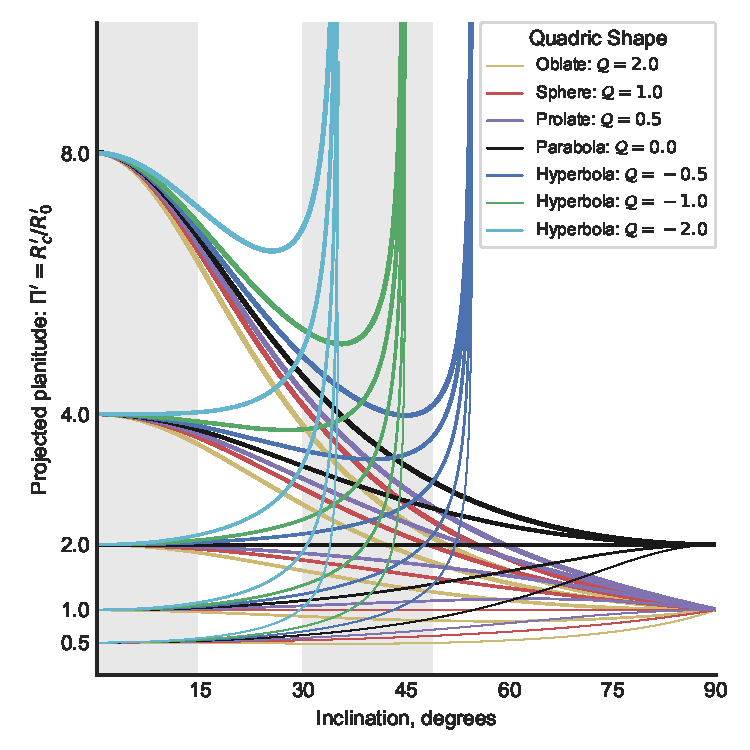
\includegraphics[width=0.5\linewidth]{./Figures/projected-Rc-vs-i} &
    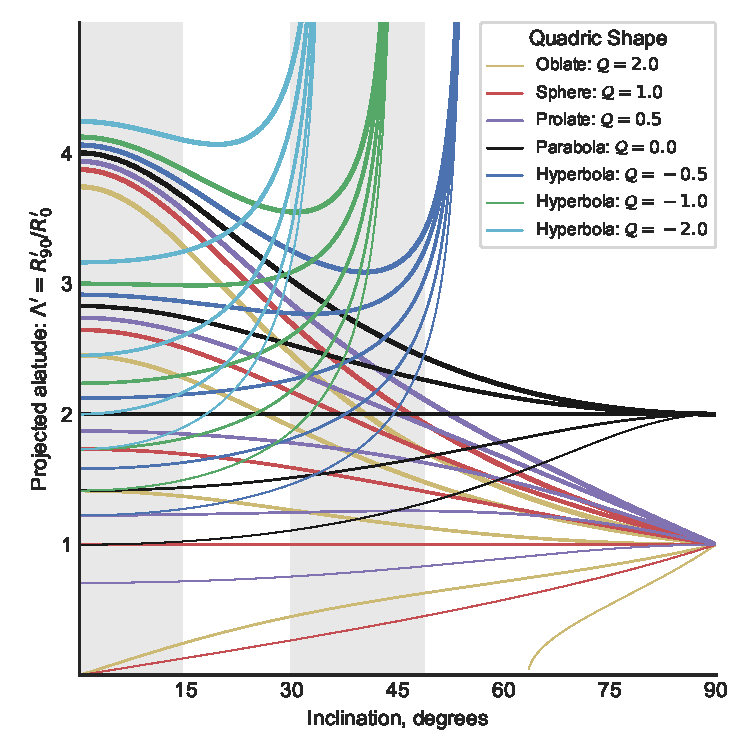
\includegraphics[width=0.5\linewidth]{./Figures/projected-R90-vs-i}
  \end{tabular}
  \caption{Efectos de la proyección sobre las cuádricas de revolución con la inclinación $|i|$. Los colores de las curvas representan variaciones en el parámetro $\Q$ de las cuádricas. El grosor de la curva indica el valor de la planitud intrínseca $\Pi$. Los rectángulos sombreados muestran cuartiles de $|\sin i|$ que se encuentran equitativamente poblados para una distribución isotrópica de orientaciones. (a) Planitud aparente $\Pi'$. (b) Alatud aparente $\Lambda'$}
  \label{fig:proj-L-P-vs-i}
\end{figure*}

\begin{figure}
  \begin{tabular}{lr}
    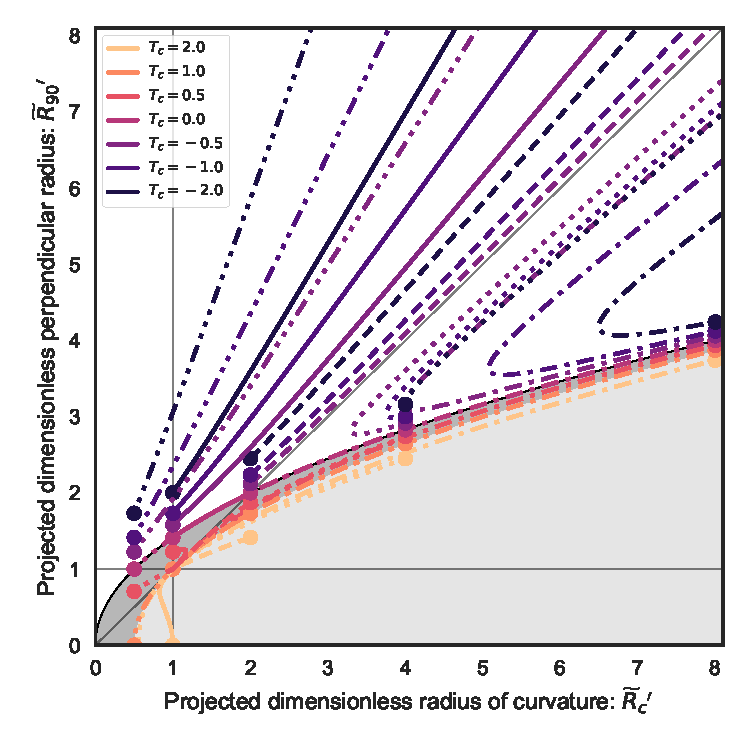
\includegraphics[width=0.5\linewidth]{./Figures/projected-R90-vs-Rc} &
    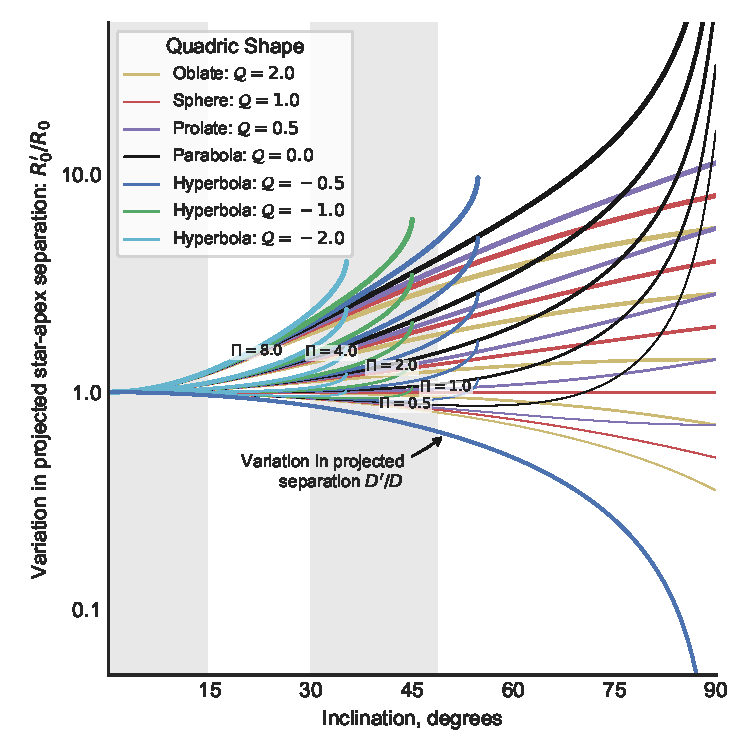
\includegraphics[width=0.5\linewidth]{./Figures/projected-R0-vs-i}
  \end{tabular}
  \caption{(a) Diagrama de diagnóstico $\Lambda'$ vs $\Pi'$ para diferentes tipos de cuádricas: esferoides oblatos (amarillo), esferoides (rojo), esferoides prolatos (morado), paraboloides (negro) e hiperboloides (azul, verde y turquesa). Cada punto de una curva representa un valor diferente de la inclinación, y se muestran explícitamente las inclinaciones múltiplos de $15^\circ$, con la forma de círculos rellenos. Las regiones sombreadas representan al tipo de cuádrica que mejor ajusta a los parámetros $(\Pi', \Lambda')$ cubiertos. La región clara para los hiperboloides, la región gris oscura para los esferoides prolatos y la región gris clara para los hiperboloides oblatos. La interfaz entre la región de hiperboloides y esferoides prolatos corresponde a los paraboloides y la región entre esferoides prolatos y oblatos a los esferoides. (b) Distacia proyectada $R'_0/R_0$ versus $|i|$.}
  \label{fig:Pip-Lambdap-diagnostic}
\end{figure}

En la figura \ref{fig:Pip-Lambdap-diagnostic}a observamos el diagrama de diagnóstico $\Pi'-\Lambda'$. Cada curva representa a una cuádrica de revolución siguiendo la misma convención que en la figura \ref{fig:proj-L-P-vs-i} para los valores de $\Q$ y $\Pi$ y variando la inclinación a lo largo de cada una de éstas, donde además el punto donde $i=0$ (cuádrica vista de canto) se marca con un punto. Las regiones sombreadas representan a cada clase de cuádrica, la zona superior más clara a los hiperboloides, la zona gris delgada a los elipsoides prolatos, la interfaz entre estas dos últimas a los hiperboloides y la zona gris inferior a los elipsoides oblatos. Se puede observar que en ningún caso las curvas cruzan de una región a otra. También se observa de nuevo que las curvas elipsoidales convergen a $(\Pi', \Lambda') = (1, 1)$, las curvas hiperbólicas a $(\Pi', \Lambda') = (+\infty, +\infty)$ y las parabólicas a $(\Pi', \Lambda') = (2, 2)$. Asimismo en la figura \ref{fig:Pip-Lambdap-diagnostic}b observamos el comportamiento de la separación aparente estrella--ápex con inclinación. En este caso se observa que para inclinaciones pequeñas $(|i| < 30^\circ)$, esta separación depende muy poco del parámetro $\Q$, siendo más importante la planitud $\Pi$. Por otro lado, para inclinaciones mayores, la separación aparente se incrementa cada vez más rápido para cuádricas abiertas $(\Q \leq 0)$, mientras que para los elipsoides la separación es cada vez más lenta e incluso puede decrecer con inclinación.

\begin{figure}
  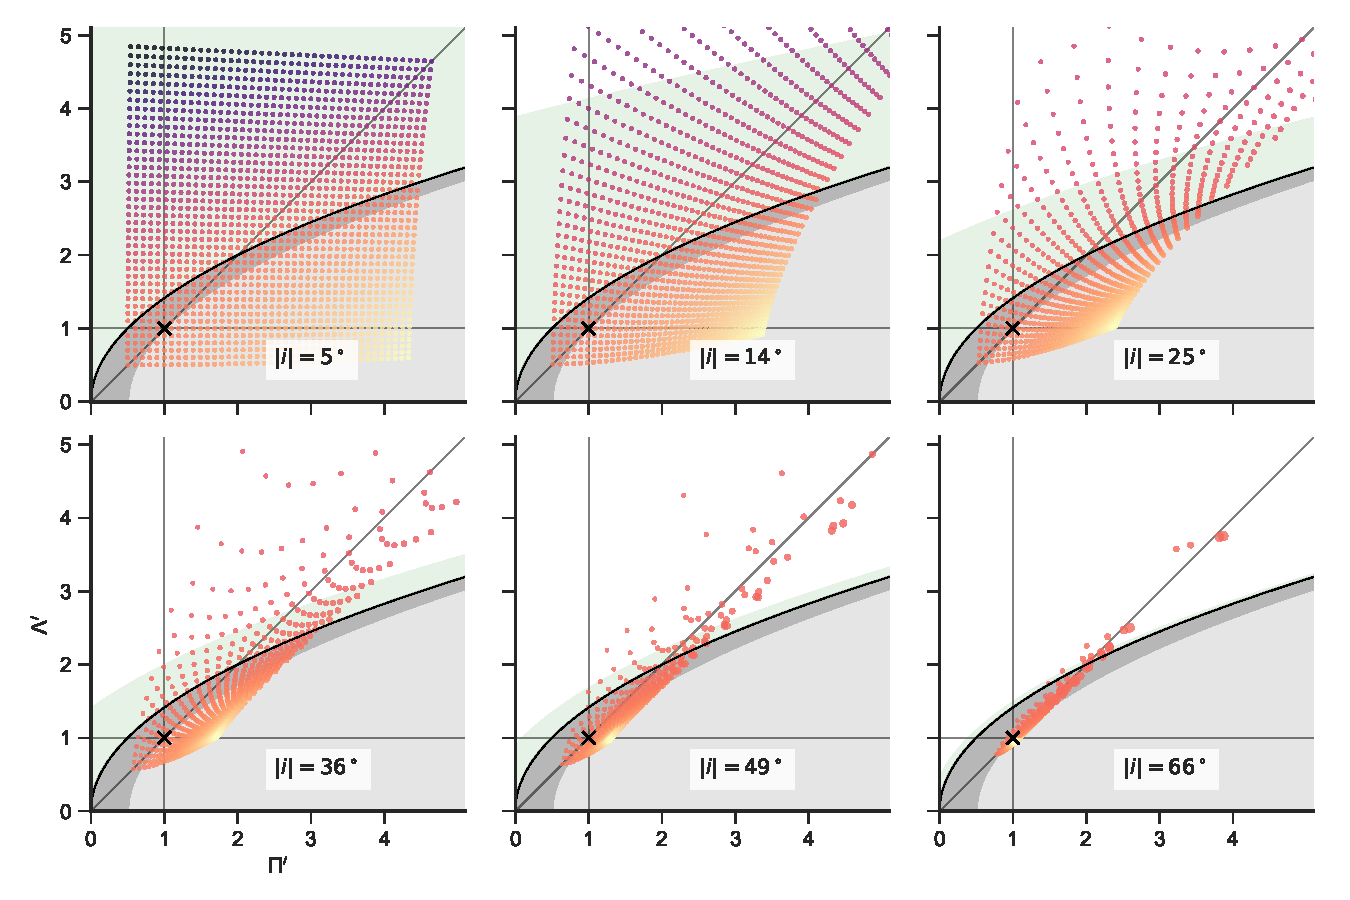
\includegraphics[width=\linewidth]{./Figures/projected-R90-Rc-snapshots}
  \caption{Efectos de la inclinación de la forma aparente de arcos cuádricos cuya planitud y alatud están uniformemente distribuídos en los rangos $\Pi = [0.5, 4.5]$, $\Lambda = [0.5, 4.5]$. En cada pánel se muestra la forma aparente incrementando la inclinación en intervalos iguales de $|\sin i|$. El collor representa el parámetro $\Q$, desde azul (menor valor de $\Q$, que representa formas más abiertas), pasando por naranja, hasta amarillo (elipsoides oblatos). El tamaño representa la distancia aparente estrella--ápex $R'_0/R_0$.}
  \label{fig:snapshots}
\end{figure}


De manera complementaria en la figura \ref{fig:snapshots} mostramos una visión complementaria del análisis de la forma aparente con la inclinación. En esta figura se toman ``capturas'' de $(\Pi', \Lambda')$ en intervalos regulares de $\sin i$. Los valores de la planitud y alatud intrínseca están uniformemente distribuídos en los intervalos $\Pi = [0.5, 4.5]$ y $\Lambda = [0.5, 4.5]$, lo que nos da un cuadrado uniformemente distribuído de valores cuando $|i| = 0$, y que se va distorsionando conforme $|i|$ se incrementa. La escala de color representa el parámetro $\Q$, incrementándose dicho parámetro desde el azúl hasta el amarillo, pasando por el naranja, mientras que el tamaño del punto es proporcional a $R'_0/R_0$. Se puede observar que todos los puntos tienden a la línea $\Pi' = \Lambda')$ a altas inclinaciones, y que los puntos azules quedan fuera del rango de la gráfica. Esto es porque a altas inclinaciones, para las formas muy abiertas ya no existe la línea tangente a la línea de visión. De hecho, la región verde sombreada es la región para la cual aun existe la línea de visión para cada inclinación y se hace cada vez más pequeña conforme la inclinación aumenta. Esta figura es meramente cualitativa, puesto que no hay razón para esperar una distribución uniforme de planitud y alatud (en el siguiente capítulo encontramos que en el modelo de capa delgada no encontramos formas cuyo parametro $\Q$ sea mayor a 1, por ejemplo).

% Utilizando las ecuaciones (\ref{eq:x0}), (\ref{eq:a-prime}) y (\ref{eq:b-prime}), utlizando la definición $D' = D\cos i$ e introduciendo la función $f(i;\theta_c)\equiv \left(1 \pm \tan^2\theta_c\tan^2i\right)^{1/2}$ obtenemos ecuaciones explícitas para los radios característicos en el sistema de referencia del plano del cielo en términos de la inclinación:
%\begin{align}
%  \frac{q'}{q} &= 1 \pm \tilde{R}_c\cot^2\theta_c\left(f(i;\theta_c) - 1\right) \\
%  \tilde{R}'_c &= \frac{\tilde{R_c}}{\cos^2if(i;\theta_c)\frac{q'}{q}} \label{eq:Rpc-quad}\\
%  \tan\theta'_c &= \frac{\tan\theta_c}{\cos if(i;\theta_c)} \label{eq:thcp-quad}\\
%  \tilde{R}'_{90} &= \left(\frac{2\tilde{R}_cf(i;\theta_c) \mp
%                    \tan^2\theta_c\frac{q'}{q}}{q'/q}\right)^{1/2}\frac{\sec %i}{f(i;\theta_c)}
%  \label{eq:Rp90-quad}
%\end{align}
%Cuando $\tilde{R}'_{90}$ es medible, entonces es posible hacer diagramas de diagnóstico como
%el de la figura \ref{fig:diagnostic} para comparar con observaciones, independientemente de cualquier modelo de choques de proa.
%\begin{figure}
%  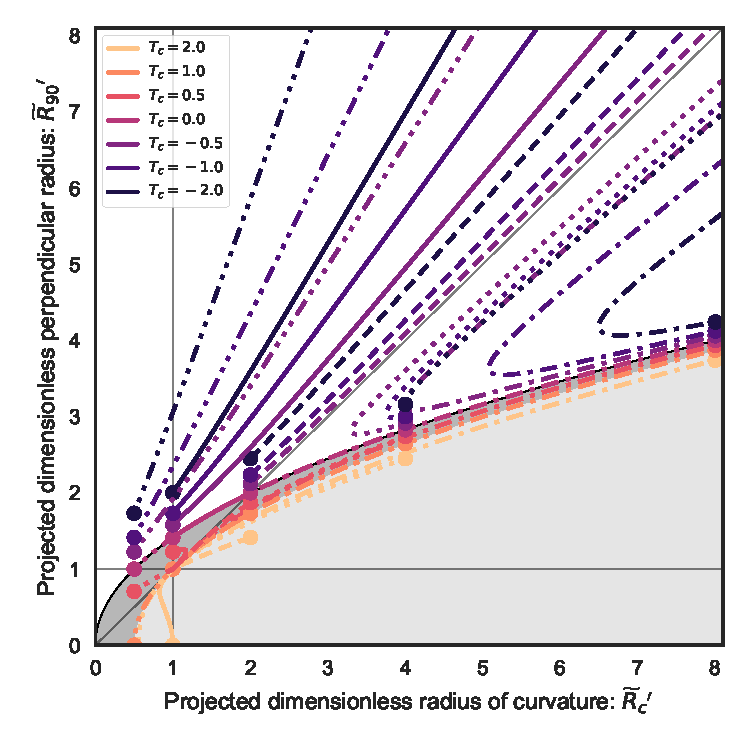
\includegraphics[width=0.5\linewidth]{./Figures/projected-R90-vs-Rc}
%  \caption{Diagrama de diagnóstico $\tilde{R}'_{90}$ vs $\tilde{R}'_c$ para las cuádricas de revolución. En la región sin sombrear se representan las superficies abiertas (hiperboloides, $\theta_c <0$), mientras que la región más oscura representa a elipsoides prolatos  $(0 < \theta_c < 45^\circ)$ y la región poco sombreada a elipsoides oblatos $(\theta_c > 45^\circ)$}
%  \label{fig:diagnostic}
%\end{figure}

\chapter{Modelo de Capa Delgada}
\label{chap:hipersonica}

\defcitealias{Canto:1996}{CRW}
\newcommand\CRW{\citetalias{Canto:1996}}

Un ejemplo más realista para la forma de los choques de proa proviene de modelos hidrodinámicos en estado estacionario de la interacción de flujos hipersónicos en el límite de capa delgada. Ejemplos clásicos son la interacción entre dos vientos de \citet{Canto:1996} (\CRW{} de aquí en adelante) y la interacción entre un viento con una corriente plano--paralela \citep{Wilkin:1996}. 
%El problema de interacción de dos vientos es de gran interés en astrofísica, y ha sido estudiado en múltiples ocasiones, principalmente mediante simulaciones hidrodinámicas. Sin embargo, cuando se toman en cuenta diversos factores, incluídos conservación de masa, momento y momento angular, el problema puede resolverse de manera algebraica.
\section{Cantidades conservadas en un flujo hipersónico de capa delgada}

Consideramos dos flujos hipersónicos, no acelerados que forman una capa estacionaria delgada formada por dos choques radiativos separados por una discontinuidad de contacto. El sistema tiene geometría cilíndrica y los vientos no tienen velocidad azimutal. Bajo estos términos, describimos la posición de la capa delgada como $R(\theta)$, donde $R$ es el radio de la capa medido a partir de la posición del origen del viento con menor momento y $\theta$ es el ángulo polar. Asumimos que el gas chocado está bien mezclado, esto implica que  tiene una sola velocidad pos--choque dada por:

\begin{align}
  \vec{v} = v_r \hat{r} + v_z \hat{z}
\end{align}

Donde el eje de simetría del sistema es paralelo a $\hat{z}$, y $\hat{r}$ es el radio cilíndrico. Definimos $\dot{M}(\theta)$, $\vec{\dot{\Pi}}(\theta)$ y $\dot{J}(\theta)$ como la tasa de pérdida de masa, la tasa de momento y la tasa de momento angular, respectivamente, de la capa delgada integradas desde $\theta=0$ hasta $\theta$. Éstas se calculan de la siguiente manera:

\begin{align}
  \vec{\dot{\Pi}}(\theta) &= \dot{\Pi}_r(\theta) \hat{r} + \dot{\Pi}_z(\theta) \hat{z} = \dot{M}\left(v_r \hat{r} + v_z\hat{z}\right) \label{eq:dot-pi}\\
  \vec{\dot{J}}(\theta) &= \vec{R}(\theta) \times \vec{\dot{\Pi}}(\theta)  \\
  \dot{M}(\theta) &= \dot{M}_w(\theta) + \dot{M}_{w1} \label{eq:dot-M}
\end{align}
Donde $\vec{R}(\theta)\equiv R(\theta)\sin\theta~\hat{r} + R(\theta)\cos\theta~\hat{z}$. Resolviendo el producto cruz y tomando su magnitud encontramos que:
\begin{align}
  \dot{J}(\theta) &= \dot{M}(\theta)R(\theta)v_\theta \label{eq:dot-J}\\
  \mathrm{donde:~} & v_\theta = v_r\cos\theta - v_z\sin\theta \label{eq:v-theta}
\end{align}

Por otro lado, al asumir estado estacionario, necesitamos que la tasa de pérdida de masa, la tasa de momento y la tasa de momento angular de la capa delgada sean iguales a aquellas inyectadas por los dos vientos. Entonces definimos estas cantidades como $\dot{M}_w$, $\dot{\Pi}_{wr}$, $\dot{\Pi}_{wz}$ y $\dot{J}_{w}$ para el viento con menor momento, y para el otro viento se utiliza la misma notación solo que utilizando el subíndice ``w1''. De esta forma tenemos que:
\begin{align}
  \dot{\Pi}_r(\theta)\hat{r} + \dot{\Pi}_z(\theta)\hat{z} &= \left[\dot{\Pi}_{wr}(\theta)+ \dot{\Pi}_{wr1}(\theta)\right]\hat{r} + \left[\dot{\Pi}_{wz}(\theta)+ \dot{\Pi}_{wz1}(\theta)\right]\hat{z} \label{eq:Pi-2} \\
  \dot{J} &=\dot{J}_w(\theta) + \dot{J}_{w1}(\theta) \label{eq:J-2}\\
  \dot{M}(\theta) &= \dot{M}_w(\theta) + \dot{M}_{w1}(\theta) \label{eq:M-2}
\end{align}

Combinando las ecuaciones (\ref{eq:dot-pi}, \ref{eq:dot-M}, \ref{eq:dot-J}, \ref{eq:Pi-2}-\ref{eq:M-2}) encontramos que:

\begin{align}
  \dot{M}(\theta)\left[v_r \hat{r} + v_z\hat{z}\right] &= \left(\dot{\Pi}_{wr}(\theta) + \dot{\Pi}_{wr1}(\theta)\right)\hat{r} +
                                                         \left(\dot{\Pi}_{wz}(\theta) + \dot{\Pi}_{wz1}(\theta)\right)\hat{z} \\
  \dot{M}(\theta)v_\theta R(\theta) &= \dot{J}_w(\theta) + \dot{J}_{w1}(\theta)
\end{align}
Y finalmente combinando con la ecuación (\ref{eq:v-theta}) resolvemos para $R(\theta)$:
\begin{align}
  R(\theta) = \frac{\dot{J}_w(\theta) + \dot{J}_{w1}(\theta)}{\left(\dot{\Pi}_{wr}(\theta) + \dot{\Pi}_{wr1}(\theta)\right)\cos\theta - \left(\dot{\Pi}_{wz}(\theta) + \dot{\Pi}_{wz1}(\theta)\right)\sin\theta} \label{eq:R-wind}
\end{align}

\section{Problema de Interacción de Dos Vientos}
\label{sec:CRW-2-winds}
Aplicamos el formalismo ya mencionado para la interacción de dos vientos radiales. El viento con menor momento se localiza en el origen, y su densidad a radio fijo varía con el ángulo polar como una ley de potencias (figura \ref{fig:isotropic-aniso}), o bien, un viento interno con densidad constante e isotrópica:
\begin{align}
  n_{An}(\theta) &=\left\lbrace
  \begin{array}{lr}
    n_0\cos^k\theta  & \mathrm{si~}\theta\leq 90^\circ \\
    0 & \mathrm{si~}\theta > 90^\circ
  \end{array}\right. \label{eq:Ancantoid-density}\\
  n_C &= n_0 \label{eq:cantoid-density}
\end{align}

Donde el índice $k$ indica el grado de anisotropía del viento ``interno''. Cuando la densidad del viento está dada por la ecuación (\ref{eq:cantoid-density}) denominamos a los choques resultantes como ``cantoides'', por \citet{Canto:1996}, mientras que si la densidad está dada por (\ref{eq:Ancantoid-density}) entonces los denominamos ``Ancantoides''. Un caso particularmente interesantes son el viento para un proplyd \citep{HA:1998}, donde $(k=1/2)$. Por el momento restringimos al viento ``externo'' como isotrópico. El problema se muestra de manera esquemática en la figura \ref{fig:crw-esquema}.

Utilizando las ecuaciones (\ref{eq:Ancantoid-density}, \ref{eq:cantoid-density}) encontramos que la tasa de pérdida de masa está dada por:

\begin{align}
  \dot{M}_w = \int^\theta_0\int^{2\pi}_0\rho_w v_w~r^2_0\sin\theta~d\theta~d\phi  \label{eq:general-inner-dot-M}
\end{align}
Donde $v_w$ es la velocidad del viento inteno, $\rho_w = n\bar{m}$  es su densidad, $n$ se obtiene de las ecuaciones (\ref{eq:Ancantoid-density}), $\bar{m}$  es la masa promedio de las partículas del viento y $r_0$ es el radio del viento al cual se alcanza la velocidad terminal $v_w$. Para un proplyd consideramos que dicho radio es el del frente de ionización.

Resolviendo (\ref{eq:general-inner-dot-M}) para vientos con densidades dadas por (\ref{eq:Ancantoid-density}, \ref{eq:cantoid-density}), encontramos que:

\begin{align}
  \dot{M}_w = \dot{M}^0_w\left\lbrace
  \begin{array}{lr}
    \left(1 - \cos^k\theta\right) & \mathrm{Ancantoides} \\
    \frac{1}{2} \left(1 - \cos\theta\right) & \mathrm{Cantoides}
  \end{array}\right. \label{eq:inner-dot-M}
\end{align}
Donde:
\begin{align}
  \dot{M}^0_w = \left\lbrace
  \begin{array}{lr}
    \frac{2\pi}{k+1}\bar{m}n_o v_w r_0^2 & \mathrm{Ancantoides} \\
    4\pi \bar{m}n_o v_w r_0^2 & \mathrm{Cantoides}
  \end{array}\right.
\end{align}

Con esto, obtenemos las tasas de momento y momento angular. Para los choques cantoides, los resultados corresponden a las ecuaciones (9-11) de \CRW{}, sin embargo, para los choques ancantoides, las tasas de momento (axial y radial) y momento angular están dados por:
\begin{align}
  \dot{\Pi}_{wz} &= \int^{\mathrm{min}(\theta, \pi/2)}_0 v_w\cos\theta~d\dot{M}_w = \frac{v_w \dot{M}^0_w}{2\left(k+2\right)}\mathrm{max}\left(1 - \cos^{k+2}\theta, 1\right) \label{eq:Pi-wz} \\
  \dot{\Pi}_{wr} &= \int^{\mathrm{min}(\theta, \pi/2)}_0 v_w\sin\theta~d\dot{M}_w = \frac{1}{2}\dot{M}^0_w v_w I_k(\theta) \\
  \dot{J}_w &= \int^{\mathrm{min}(\theta, \pi/2)}_0 |\vec{R} \times \vec{v}_w|d\dot{M}_w = 0 \label{eq:inner-dot-J}
\end{align}

Donde:
\begin{align}
  I_k(\theta) = \int^{\mathrm{min}(\theta, \pi/2)}_0 \cos^k\theta \sin^2\theta~d\theta \label{eq:Ikt}
\end{align}
 Esta última integral tiene una solución analítica en términos de una función hipergeométrica de la forma ${}_2F_1\left(-\frac{1}{2}; \frac{1+k}{2}; \frac{3+k}{2}; \cos^2\theta\right)$. En el caso particular $k=1/2$, este resultado se ``simplifica'' a una integral de segundo tipo de la forma $E\left(\frac{\theta}{2} | 2\right)$, pero es más sencillo calcularla de manera numérica. La tasa de momento angular para el viento interior es cero debido a que éste se mide respecto al origen, donde se localiza la fuente con menor momento. En este punto los vectores de posición y velocidad para un valor de $\theta$ dado son paralelos.

Para el viento exterior utilizamos las ecuaciones (12-15) y (19-22) de \CRW{} sin cambiar, pero las incluímos en las siguientes secciones por completez.

\subsection{Interacción con un viento esférico isotrópico}
\label{sec:mod-isotropic}

\begin{figure*}
  \begin{tabular}{lr}
    \includegraphics[width = 0.55\linewidth]{./Figures/cantoid-ancantoid-shape-bfixed} &
    \includegraphics[width=0.55\linewidth]{./Figures/ancantoid-shape}
  \end{tabular}
  \caption{Forma de choques de proa de vientos en interacción. Las coordenadas están normalizadas con $D$, la distancia entre las fuentes de los vientos. La fuente del viento más débil se localiza en el origen $(0, 0)$, mientras que la otra fuente se localiza en $(1, 0)$, ambas marcadas con puntos negros. En (a) los choques de proa mostrados tienen un valor del parámetro $\beta = 0.01$ fijo, mientras que el índice de anisotropía $k$ varía desde 0 hasta 3, mostrados en escala de colores verdes. El choque cantoide con $\beta=0.01$ se muestra en negro. Nótese que el choque ancantoide con $k=0$ es más cerrado en las alas que el tipo cantoide, debido a que en los choques ancantoides la densidad del viento cae a cero cuando $\theta \geq 90^\circ$, mientras que en los cantoides la densidad del viento es constante para toda $\theta$. En (b) el parámetro de anisotropía $k$ es fijo con valor de $1/2$, mientras que el parámetro $\beta$ varía desde $10^{-3}$ hasta $0.99$. La distancia al ápex $R_0$ se incrementa conforme $\beta$ crece, llegando al valor asintótico de $R_0/D = 0.5$ cuando $\beta\to 1$. Lo mismo sucede con el radio de curvatura y $R_{90}$. Algo notable es que en los choques ancantoides aun en el caso límite $\beta=1$, la forma del choque también es curva, debido a que la densidad del viento interior cae con $\theta$ y fuera del eje de simetría el momento del viento exterior es mayor.}
\end{figure}

En este caso tomamos como variable independiente al ángulo polar medido a partir de la posición de la fuente del viento externo, denotado por $\theta_1$. De esta forma las tasas de pérdida de masa, momento y momento angular quedan como sigue:

\begin{align}
  \dot{M}_{w1} &= \frac{M^0_{w1}}{2}\left(1 - \cos\theta_1\right)\\
  \dot{\Pi}_{wz1} &= -\frac{v_{w1}\dot{M}^0_{w1}}{4}\sin^2\theta_1\\
  \dot{\Pi}_{wr1} &= \frac{v_{w1}\dot{M}^0_{w1}}{4}\left(\theta_1 - \sin\theta_1\cos\theta_1\right)\\
  \dot{J}_{w1} &= \int^{\theta_1}_0 R(\theta)v_{w1}\sin(\pi-\theta-\theta_1)~d\dot{M}_{w1} \label{eq:J1}
\end{align}

Utilizando la ley de los senos (ver figura \ref{fig:crw-esquema}), la ecuación (\ref{eq:J1}) queda como sigue:

\begin{align}
  \dot{J}_{w1} &= Dv_{w1}\int^{\theta_1}_0 \sin\theta_1~d\dot{M}_{w1} =
                 \frac{v_{w1}\dot{M}^0_{w1}}{4}\left(\theta_1 - \sin\theta_1\cos\theta_1\right) D \label{eq:J1-iso}
\end{align}

Por otro lado, de la figura \ref{fig:crw-esquema}, podemos deducir la siguiente relación geométrica entre $R(\theta)$,
$\theta$ y $\theta_1$:
\begin{align}
  \frac{R(\theta)}{D} &= \frac{\sin\theta_1}{\sin(\theta+\theta_1)} \label{eq:R-geometric}
\end{align}

Combinando las ecuaciones (\ref{eq:R-wind}, \ref{eq:Pi-wz} - \ref{eq:J1-iso}, \ref{eq:R-geometric}) obtenemos una ecuación implícita que nos indica la dependencia de $\theta_1$ con $\theta$:

\begin{align}
  \theta_1\cot\theta_1 -1 = 2\beta I_k(\theta)\cot\theta - \frac{2\beta}{k+2}\left(1 - \cos^{k+2}\theta\right) \label{eq:th1-th} 
\end{align}
Donde en este caso, la condición de equilibrio de presiones RAM implica que la tasa de momentos $\beta$ ahora está definida como sigue:

\begin{align}
  \beta\dot{M}^0_{w1}v_{w1} = 2(k+1) \dot{M}^0_{w}v_{w}
\end{align}
Sin embargo, (\ref{eq:th1-th}) solo aplica en el rango $0 < \theta \leq \pi/2$. Cuando $\theta > \pi/2$ la relación entre $\theta$ y $\theta_1$ es:

\begin{align}
  \theta_1\cot\theta_1 - 1 = 2\beta\left(I_k(\pi/2)\cot\theta - \frac{1}{k+2}\right) \label{eq:th1-th-far-wings}
\end{align}

Donde:
\begin{align}
I_k(\pi/2) = \frac{\pi}{4}\frac{\Gamma\left(\frac{1+k}{2}\right)}{\Gamma\left(\frac{4+k}{2}\right)} 
\end{align}
y $\Gamma$ es la función Gamma usual.

\subsection{Interacción de un viento esférico isotrópico con un viento plano--paralelo (Choques Wilkinoides)}
\label{sec:wilkinoids}
\begin{figure*} \includegraphics[width=0.6\linewidth]{./Figures/cantoid-wilkinoid-shape}
  \caption{Forma de choques cantoides y el choque wilkinoide. Las coordenadas están normalizadas con la distancia al ápex $R_0$. El choque wilkinoide se muestra en negro y los choques cantoides en escala de azul, con $\beta$ variando desde $10^{-3}$ hasta 0.08. Nótese que el choque wilkinoide se comporta como el caso asíntótico de los choques cantoides cuando $\beta\to 0$.}
\end{figure*}
En este caso las tasas de pérdida de masa, de momento y momento angular del viento plano--paralelo con velocidad $v_a$ y densidad uniforme $\rho_a$ quedan como sigue:
\begin{align}
  \dot{M}_{w1} &= \pi \rho_a v_a R^2 \sin^2\theta\\
  \dot{\Pi}_{wz1} &= - \pi\rho_a v^2_a R^2 \sin^2\theta\\
  \dot{\Pi}_{wr1} &= 0 \\
  \dot{J}_{w1} &= \int^r_0 r'v_a \sin\theta~d\dot{M}_{w1} = \frac{2}{3}\pi\rho_a v_a^2 R^3 \sin^3\theta 
\end{align}
Sustituyendo estas ecuaciones en (\ref{eq:R-wind}) junto con (\ref{eq:inner-dot-M}-\ref{eq:inner-dot-J}) para vientos tipo cantoides $(k=0)$ obtenemos lo siguiente:
\small
\begin{align}
  R = \frac{\frac{2}{3}\pi\rho_a v_a R^3 \sin^3\theta}{\frac{\dot{M}^0_w v_w}{4}\left(\theta-\sin\theta\cos\theta\right)\cos\theta
  - \left(\frac{\dot{M}^0_w v_w}{4}\sin^2\theta - \pi\rho_a v^2_a R^2 \sin^2\theta\right)\sin\theta}
\end{align}
\normalsize
La condición de equilibrio de presión en este caso nos lleva a la siguiente relación:
\begin{align}
  \frac{\dot{M}^0_w v_w}{4\pi R^2_0} = \rho_a v^2_a \label{eq:Wilkin-stagnation}
\end{align}
Por tanto:
\begin{align}
  R/R_0 = \frac{\frac{2}{3}\left(R/R_0\right)^3 \sin^3\theta}{\left(\theta-\sin\theta\cos\theta\right)\cos\theta
  - \left(\sin^2\theta - \left(R/R_0\right)^2 \sin^2\theta\right)\sin\theta}
\end{align}
Resolviendo para $R/R_0$ encontramos que:
\begin{align}
  R = R_0\left[\csc^2\theta\left(1 - \theta\cot\theta\right)\right]^{1/2} \label{eq:R-Wilkin}
\end{align}


\section{Forma ``verdadera'' de los choques cantoides, ancantoides y wilkinoides}

\begin{figure*}
  \includegraphics[0.7\linewidth]{./Figures/Pi-vs-Lambda}
  \caption{Forma verdadera de los choques cantoides, ancantoides y wilkinoides. En cada línea, $\beta$ varía en el rango $[0, 1]$, y los parámetros $(\Pi, \Lambda)$ fueron calculados de acuerdo a los resultados del apéndice \ref{app:derivation-radii}. Los círculos del color de las líneas representan valores particulares de $\beta$: $10^{-3}$, $10^{-2}$, 0.1 y 0.5, y con la diferencia de que el coeficiente de segundo orden de la ecuación \ref{eq:CRW-Rc} para la planitud $\Pi$ fue obtenido de manera numérica con el fin de utilizar este método para encontrar la planitud aparente con la ecuación \ref{eq:Rc-prime}}
  \label{fig:true-Pi-Lambda}
\end{figure*}
Para los tres tipos de formas de choques de proa que utilizamos en este trabajo (cantoides, ancantoides y wilkinoides), calculamos su correspondiente alatud y planitud. Para los choques ancantoides obtenemos lo siguiente. El procedimiento detallado se puede consultar en el apéndice \ref{app:derivation-radii}:

\begin{align}
  \Lambda &= \frac{\left(3\xi_k\right)^{1/2}\left(1+\beta^{1/2}\right)} {\left(1+\frac{1}{5}\xi_k\beta\right)^{1/2}\left(1-\xi_k\beta\right)} \label{eq:CRW-R90}\\
  \Pi &= \left|1 - 2\frac{R_{\theta\theta, 0}}{R_0}\right|^{-1} \label{eq:CRW-Rc}\\
  \mathrm{Donde:~} R_{\theta\theta, 0} &= \frac{C_{k\beta}}{1+\beta^{1/2}} + \frac{1 + 2\beta^{1/2}}{3} \label{eq:2-order}
\end{align}
Donde $\xi_k \equiv \frac{2}{k+2}$ y $C_{k\beta}$ son parámetros que se introduce por conveniencia en el apéndice \ref{app:derivation-radii}.

Para los choques cantoides la planitud y alatud son equivalentes al resultado del choque ancantoide con $k=0$, pero se muestran a continuación por completez:

\begin{align}
  \Pi &= \frac{5}{3\left(1-\beta^{1/2}\right)}\label{eq:cantoid-planitude}\\
  \Lambda &= \frac{\sqrt{3}}{\left(1 + \frac{1}{5}\beta\right)^{1/2}\left(1 - \beta^{1/2}\right)} \label{eq:cantoid-alatude}
\end{align}

Por último, el radio en el ápex, la planitud y alatud para los choques wilkiniodes es:

\begin{align}
   R_0 &= \left(\frac{\dot{M}^0_w v_w}{4\pi \rho_a v^2_a}\right)^{1/2} \\
  \Lambda &= \sqrt{3} \label{eq:R90-Wilkin} \\
  \Pi &= \frac{5}{3} \label{eq:Rc-Wilkin}
\end{align}

$R_0$ en este caso se obtiene directamente de la ecuación (\ref{eq:Wilkin-stagnation}), mientras que $\Pi$ y $\Lambda$ se obtienen tomando el límite $\beta\to 0$ en las ecuaciones (\ref{eq:cantoid-planitude}, \ref{eq:cantoid-alatude}), aunque $\Lambda$ también puede obtenerse evaluando la ecuación (\ref{eq:R-Wilkin}) en $\theta=\pi/2$.

En la figura \ref{fig:true-Pi-Lambda} se muestran los resultados de las ecuaciones (\ref{eq:CRW-R90}-\ref{eq:Rc-Wilkin}) en forma de diagrama $\Lambda-\Pi$. Los choques tipo cantoides ocupan en este diagrama una curva, donde cada punto de ésta representa un valor distinto de $\beta$, cuyo rango es $(0, 1)$, y está representada en color negro. Los choques ancantoides ocupan diferentes curvas, una por cada valor del índice de anisotropía $k$, y se representan por curvas con diferente tonalidad de verde, mientras que los choques wilkinoides ocupan un solo punto en este diagrama, representado por el círculo amarillo.

La tendencia general de los choques cantoides y ancantoides es que conforme se incrementan $\beta$ y $k$, también se vuelven más abiertos y más planos en el aṕex ($\Pi$ y $\Lambda$ incrementan), siendo el choque tipo cantoide el más abierto a un valor de $\beta$ dado. Como ya hemos mencionado, el choque tipo cantoide y el tipo ancantoide con $k=0$ son muy similares, excepto que el choque cantoide es más abierto en las alas $(\theta > 90^\circ)$ debido al soporte que da hacia atrás el viento interior. Sin embargo, como su comportamiento es igual para $\theta \leq 90^\circ$, por tanto, no hay diferencia entre estos dos tipos de choques en este diagrama. Todos los choques se encuentran ya sea en la región de esferoides prolatos (región gris oscura) o hiperboloides (región clara), ninguno en la región de esferoides oblatos (ver figura \ref{fig:Pip-Lambdap-diagnostic}a). Los choques tipo esferoide prolato son los que tienen valores de $\beta$ pequeños, y la transición hacia hiperboloide se da cunado $\beta \sim 0.01$ para los choques cantoides y ancantoides con parámetro $k$ pequeño. Esta transición a los hiperboloides se recorre para $\beta$ mayor conforme el parámetro $k$ se incrementa. Esto contrasta con el caso de las cuádricas puras, que siempre permanecen en la misma región, pero esto se debe a que las formas de los choques de proa son más complejas que una cuádrica de revolución: mientras que la forma de la ``cabeza'' del choque (la región cercana al ápex) puede aproximarse bien con una variedad de cuádricas, la forma de las alas lejanas siempre es más parecida a un hiperboloide (ver figura ). El choque wilkinoide se ubica en el límite $\beta\to 0$ de la curva de los choques cantoides, como era de esperarse, y se ubica en la región de esferoides prolatos. Otro detalle que puede apreciarse en esta figura es que todas las curvas (al menos para $\beta$ pequeña) se aglomeran cerca de la diagonal $\Pi \simeq \Lambda$ con la tendencia de que para anisotropía grande, $\Lambda > \Pi$, existe ena región donde hay una degeneración entre $\beta$ y $k$ que se rompe para $\beta$ grande.

Todo esto funciona para la forma verdadera de los choques de proa, que corresponde a cuando son vistos de canto $(i=0)$. La alatud y planitud verdaderas no toman en cuenta el comportamiento de las alas lejanas $(\theta > 90^\circ)$. De hecho, para un choque dado, hay dos formas de calcular el ángulo de las cuádricas $\theta_Q$. Una es a partir de los parámetros $(\Pi, \Lambda)$ utilizando las ecuaciones (\ref{eq:conic-parameter-a-b}, \ref{eq:thc}, \ref{eq:quadric-parameter-pi-lambda}):

\begin{align}
  \theta^{\mathrm{head}}_Q = sgn\left(2\Pi - \Lambda^2\right)~\tan^{-1}\left|2\Pi-\Lambda^2\right|
\end{align}

La segunda manera es a partir de estimar el ángulo asintótico $\theta_\infty$:

\begin{align}
  \theta^{\mathrm{tail}}_Q = \theta_\infty - \pi
\end{align}

Donde $\theta_\infty$ puede obtenerse a partir de la ecuación (28) de \CRW{} para los choques cantoides:

\begin{align}
  \theta_\infty - \tan\theta_\infty = \frac{\pi}{1-\beta}
\end{align}

Mientras que para los choques ancantoides utilizamos la ecuación (\ref{eq:th1-theta-far-wings}) utilizando la condición $\theta_\infty + \theta_{1\infty} = \pi$:

\begin{align}
  \theta_\infty - \left(\frac{k+2(1-\beta)}{k+2}\right)\tan\theta_\infty = \pi + 2\beta I_k(\pi/2)
\end{align}

Como las soluciones a la forma de los choques de proa, tanto cantoides como ancantoides solo ajustan parcialmente a una cuádrica de revolución, entonces $\theta^{\mathrm{head}}_Q \neq \theta^{\mathrm{tail}}_Q$. Esta discrepancia se vuelve relevante al momento de obtener la forma aparente,ya que en este caso la región del choque que es tangente a la línea de visión se aleja del ápex y se acerca a las alas lejanas conforme se incrementa la inclinación.

\section{Obtención de la Forma Aparente}

A continuación aplicamos el formalismo desarrollado en la sección \S \ref{sec:projection} a las formas de los choques de proa obtenidos en este capítulo para obtener tanto la forma aparente como la planitud y alatud aparentes.

En la figura \ref{fig:apparent-cantoid} mostramos la forma aparente de choques tipo cantoides y wilkinoides, y mostramos como referencia un paraboloide confocal cuya forma aparente no cambia con la inclinación (ver \S \ref{sec:pi-lambda-quadric}), mientras que la figura \ref{fig:apparent-ancantoid}} muestra la forma aparente de choques ancantoides.

\begin{figure}
  \includegraphics[width=\linewidth]{./Figures/cantoid-apparent-shape}
  \caption{Forma aparente de diferentes choques de proa en intervalos de inclinación de $15^\circ$: (a) Paraboloide confocal. (b) Wilkinoide. (c) Cantoide $\beta=0.005$. (d) Cantoide $\beta=0.01$}
  \label{fig:apparent-cantoid}
\end{figure}

\begin{figure}
  \includegraphics[width=\linewidth]{./Figures/cantoid-apparent-shape}
  \caption{Extensión de la figura \ref{fig:apparent-cantoid} para choques de proa no isotrópicos (ancantoides): (a) $\beta=0.005$, $k=1/2$. (b) $\beta=0.01$, $k=1/2$. (c) $\beta=0.005$, $k=3$. (d) $\beta=0.01$, $k=3$}
  \label{fig:apparent-ancantoid}
\end{figure}

Se muestra una tendencia general en donde las alas son sistemáticamente más abiertas para altas inclinaciones. Sin embargo, en el caso de los choques Wilkinoides se muestra el comportamiento opuesto, aunque los cambios son muy sutiles. El caso de la figura \ref{fig:apparent-ancantoid}}a, donde se muestra un choque tipo ancantoide con $\beta=0.005$ y $k=1/2$ se observa que para inclinaciones menores a $60^\circ$, las alas cercanas $(\theta\sim 90^\circ)$ se cierran sutilmente, y luego se abren más para inclinaciones mayores.

En la figuras \ref{fig:th0-isotropic} y \ref{fig:th0-anisotropic} mostramos la solución a las ecuaciones (\ref{eq:th-0}, ref{eq:R0p}) para el modelo de capa delgada, junto con el factor de escalamiento $R'_0/R_0$ en función de la inclinación. En estas figuras se observa que el radio aparente en el ápex siempre aumenta con la inclinación, mostrando un crecimiento más rápido para choques más abiertos, pero un incremento mayor para choques más cerrados; ésto debido a que en los choques más cerrados la inclinación máxima donde aun existe una línea tangente es mayor.

\begin{figure}
  \includegraphics[width=\linewidth]{./Figures/cantoid-th0-vs-i}
  \caption{(a) Soluciones a la ecuación (\ref{eq:th-0}) en función de la inclinación para choques de proa del modelo de capa delgada y viento interior isotrópico (cantoides y wilkinoides). (b) Soluciones a la ecuación (\ref{eq:R0p}) en función de la inclinación normalizadas con $R_0$.}
  \label{fig:th0-isotropic}
\end{figure}

\begin{figure}
  \includegraphics[width=\linewidth]{./Figures/ancantoid-th0-vs-i}
  \caption{(a) Soluciones a la ecuación (\ref{eq:th-0}) en función de la inclinación para choques de proa del modelo de capa delgada y viento interior anisotrópico (ancantoides) para dos índices de anisotropía: $k=1/2$ (arriba) y $k=3$ (abajo). (b) Soluciones a la ecuación (\ref{eq:R0p}) en función de la inclinación normalizadas con $R_0$.}
  \label{fig:th0-anisotropic}
\end{figure}

Las soluciones a las ecuaciones (\ref{eq:th90}, \ref{eq:R90p}) para el modelo de capa delgada se muestran en las figuras \ref{fig:t90-isotropic}, \ref{eq:t90-anisotropic}. Se observa que la alatud aparente se incrementa abruptamente cuando la inclinación se aproxima a la inclinación máxima, excepto en el caso wilkinoide, donde la alatud disminuye con inclinación muy lentamente.

\begin{figure}
  \includegraphics[width=\linewidth]{./Figures/cantoid-th90-vs-i}
  \caption{(a) Soluciones a la ecuación (\ref{eq:th90}) en función de la inclinación para choques de proa del modelo de capa delgada y viento interior isotrópico (cantoides y wilkinoides). (b) Alatud aparente en función de la inclinación, obtenida a a partir del cociente de las soluciones de las ecuaciones (\ref{eq:R90p}, \ref{R0p})}
  \label{fig:t90-isotropic}
\end{figure}

\begin{figure}
  \includegraphics[width=\linewidth]{./Figures/ancantoid-th90-vs-i}
  \caption{(a) Soluciones a la ecuación (\ref{eq:th90}) en función de la inclinación para choques de proa del modelo de capa delgada y viento interior anisotrópico (ancantoides) para dos índices de anisotropía: $k=1/2$ (arriba) y $k=3$ (abajo). (b) Alatud aparente en función de la inclinación, obtenida a a partir del cociente de las soluciones de las ecuaciones (\ref{eq:R90p}, \ref{eq:R0p})}
  \label{fig:t90-anisotropic}
\end{figure}

La planitud aparente se obtuvo a partir de realizar ajustes polinómicos en $\theta^2$ a la forma aparente $R'(\theta')$ para calcular el coeficiente de segundo orden $R'_{\theta'\theta', 0}$ y posteriormente utilizar las ecuaciones (\ref{eq:Rc-prime}, \ref{eq:R0p}). 

Su comportamiento con inclinación se muestra en la figura \ref{fig:Pi-vs-inclination}. Aquí se observa un comportamiento similar al de la alatud aparente; sin embargo, en la figura \ref{fig:Pi-vs-inclination}b, donde el pararámetro de anisotropía es $k=1/2$, se observa una pequeña caída en la planitud justo antes de llegar a la inclinación máxima. 

\begin{figure}
  \includegraphics[width=\linewidth]{./Figures/Pi-vs-i}
  \caption{Soluciones a la ecuación \ref{eq:Rc-prime} para obtener la planitud aparente en función de la inclinación en el modelo de capa delgada para: (a) viento interno isotrópico (cantoides y wilkinoides) y viento interno anisotrópico (ancantoides) con índice de anisotropía de (b) $k=1/2$ y (c) $k=3$.}
  \label{fig:Pi-vs-inclination}
\end{figure}

Por último, mostramos en la figura \ref{fig:Lambda-Pi-diagram} los diagramas $\Lambda'-\Pi'$ para diferentes tipos de choques de proa. Cada curva representa un choque de proa con parámetros $(\beta, k)$ fijos donde la inclinación varía de un punto a otro a lo largo de la curva. El comportamiento de estos choques de proa se diferencia del de las cuádricas de revolución, mostrado en la figura \ref{fig:Pip-Lambdap-diagnostic}a. En este caso, las curvas no están confinadas a una sola región: para inclinaciones bajas, la mayoría de las curvas ajustan mejor a la forma de elipsoides prolatos, a excepción de las curvas con parámetro $\beta$ alto $(\beta \gtrsim 0.01)$, mientras que para altas inclinaciones la forma ajusta mejor a hiperboloides. Esto se debe a la tensión que existe entre la forma de la cabeza y de la cola (figura ).

La curva del choque wilkinoide se muestra en color blanco, y tiene un comportamiento menos interesante que otras curvas: simplemente se mueve desde $(5/3, \sqrt{3})$ hasta $(3/2, \sqrt{8/3})$. Aunque se ubica en la región de elipsoide prolato, el hecho de que $\theta_\infty$ sea de $180^\circ$ sugiere que la forma de las alas lejanas sea más parecido al de un paraboloide. Pero converge en $(3/2, \sqrt{8/3})$ en vez de en $(2, 2)$ porque las alas lejanas son asintóticamente cúbicas en vez de cuadráticas.

La densidad de marcas a lo largo de una curva nos indican la probabilidad de observar dicha porción de ésta, si asumimos una distribución isotrópica de ángulos de visión. Se puede observar que la densidad de marcas usualmente se concentra al inicio de cada curva, cerca de $i=0^\circ$, y este efecto se intensifica cuando $\beta$ es pequeño.

\begin{figure}
  \begin{tabular}{lll}
    (a) & (b) & (c) \\
    \includegraphics[width=0.33\linewidth]{./Figures/ancantoid-R90-vs-Rc-a} & \includegraphics[width=0.33\linewidth]{./Figures/ancantoid-R90-vs-Rc-b}   &                            \includegraphics[width=0.33\linewidth]{./Figures/ancantoid-R90-vs-Rc-lobeta-a}                                             
  \end{tabular}
  \caption{Diagramas planitud-ataud para las soluciones del modelo de capa delgada. Los círculos de colores indican la forma intrínseca para cada modelo $(i=0^\circ)$. Las líneas muestran la solución a este mismo modelo en función de la inclinación. Las marcas más pequeñas corresponden a inclinaciones igualmente espaciadas de $|\sin i|$. El modelo wilkinoide se muestra en color blanco. (a) Soluciones para los modelos cantoide (azul) y ancantoide $k=0.5$ (rojo) para $\beta=[0.001, 0.003, 0.01, 0.03, 0.1, 0.3]$. (b) Soluciones para modelos ancantoides $k=3$ (naranja) y $k=0$ (morado). (c) Igual que (a) pero aumentada para mostrar la convergencia de los modelos cantoides hacia el modelo wilkinoide conforme $\beta\to 0$ utilizando como referencia $\beta=[10^{-3}, 10^{-4}, 10^{-5}]$.}
  \label{fig:Lambda-Pi-diagram}
\end{figure}

\chapter[Resultados Obtenidos]{Resultados obtenidos para los proplyds ``clásicos''}
\label{chap:proplyds}
\thispagestyle{empty}
Probamos nuestro modelo descrito en los capítulos anteriores en una muestra de proplyds pertenecientes a la Nebulosa de Orión (ONC) que presentan un choque de proa. En la figura \ref{fig:proplyds-map} se muestran los proplyds que pertencen a nuestra muestra.

En todos los casos no fue posible medir el radio característico $R_{90}$ debido a que el brillo de la cáscara decae con el ángulo polar $\theta$ y no es detectable para ángulos del orden de $60^\circ$. Sin embargo, a continuación mostraremos la metodología para obtener la inclinación más probable de cada choque, así como los parámetros del modelo de cada uno de éstos que nos indican su forma intrínseca. Los resultados mostrados en este capítulo forman parte de un artículo por publicar.

\begin{figure*}
  \centering
    \includegraphics[width=\linewidth]{./Figures/LV-full-field-annotated}
    \caption{Imagen de la parte central de la Nebulosa de Orión donde se ubican los proplyds de nuestra muestra. Las cruces color cyan corresponden a las mediciones de la forma aparente para cada choque de proa. Los círculos amarillos marcan la posición de cada proplyd y la ``x'' roja corresponde a la posición de la estrella ionizante \thC{}. Los círculos negros ilustran de manera esquemática el radio de curvatura de cada choque.}
    \label{fig:proplyds-map}
\end{figure*}

\section{Metodología para la medición de la forma aparente.}
\label{sec:methodology}
Se utilizaron imágenes en el filtro de [\Ion{O}{III}] de la cámara WPC2 del Telescopio Espacial Hubble (HST). Se utilizaron las herramientas del programa DS9 para análisis de imágenes astronómicas para trazar la posición de \thC{} y de cada uno de los proplyds de la muestra. La posición y la forma de los choques de proa fue trazada con una serie de marcas a lo largo del choque. Las coordenadas de las marcas fueron guardadas en un archivo y luego procesadas para tener las coordenadas del choque en el sistema de referencia del proplyd (Figura \ref{fig:proplyds-map}). El radio de curvatura aparente se obtiene haciendo un ajuste de mínimos cuadrados de la forma de un círculo de las mediciones obtenidas. $R_0$ se obtiene como la distancia a lo largo del eje $x$ entre el proplyd y el ajuste circular dentro del rango de las coordenadas de las mediciones. 

\subsection{Medición de incertidumbres}

Para saber qué tan confiables son las coordenadas de las mediciones, se realizó el procedimiento siguiente: Del total de mediciones realizadas para cada proplyd, se crearon varias sub-muestras donde se utilizamos aproximadamente las dos terceras partes de las mediciones, pero dejando un mínimo de cuatro puntos, y se procedió a calcular los radios característicos para cada sub-muestra, y comprobar qué tanto se desvían estas mediciones de la original. En la figura \ref{fig:char-radii-obs} se muestran ejemplos de dichas sub-muestras para algunos proplyds.


\begin{figure*}
  \centering
  \setkeys{Gin}{width=0.33\linewidth}%, trim=10 30 55 62.5}
\begin{tabular}{@{}c@{}c@{}c@{}}
 
Todos los puntos & Primera sub-muestra & Segunda sub-muestra \\ \includegraphics[clip]{./Programs/LV-bowshocks-xyfancy-positionswill-177-341} & \includegraphics[clip]{./Programs/Multi-Fit/samp00/LV-bowshocks-xyfancy-positionssamp00-177-341} &
\includegraphics[clip]{./Programs/Multi-Fit/samp01/LV-bowshocks-xyfancy-positionssamp01-177-341} \\
\includegraphics[clip]{./Programs/LV-bowshocks-xyfancy-positionswill-LV4} & \includegraphics[clip]{./Programs/Multi-Fit/samp00/LV-bowshocks-xyfancy-positionssamp00-LV4} & \includegraphics[clip]{./Programs/Multi-Fit/samp01/LV-bowshocks-xyfancy-positionssamp01-LV4} \\
\includegraphics[clip]{./Programs/LV-bowshocks-xyfancy-positionswill-168-328} &  \includegraphics[clip]{./Programs/Multi-Fit/samp00/LV-bowshocks-xyfancy-positionssamp00-168-328} & \includegraphics[clip]{./Programs/Multi-Fit/samp01/LV-bowshocks-xyfancy-positionssamp01-168-328}
\end{tabular}
\caption{Ejemplos de incertidumbres sistemáticas en los ajustes circulares a la forma de los choques para tres fuentes (desde la línea superior hasta la inferior): 177-341, LV4 y 168-328. La columna de la izquierda muestra el ajuste a todos los puntos identificados en el borde de la cáscara, donde el número y el espaciamiento de los puntos es una medida subjetiva de nuestra confianza al trazar el borde de cada cáscara. Las dos columnas restantes muestran ajustes a sub-muestras seleccionadas aleatoriamente que contienen 2/3 partes de los puntos de la muestra original para cada cáscara.}
\label{fig:char-radii-obs}
\end{figure*}

\section{Resultados Empíricos.}

Los radios característicos obtenidos para la muestra original y para las submuestras se muestran en la figura \ref{fig:obs-diagnostic}. En cada pánel se utiliza un valor fijo para el parámetro de anisotropía $k$. De estas figuras se pueden obtener la tasa de momentos $\beta$ y la inclinación $i$ para un grado de anisotropía dado por inspección visual al encontrar intersecciones entre las curvas teóricas y las barras radiales de las incertidumbres de cada proplyd. En general algunas observaciones cualitativas que se encuentran son: Los proplyds con planitud mayor, LV4 y LV2b ajustan mejor a modelos donde el parámetro de anisotropía es bajo. LV2, quien tiene la planitud aparente más baja de toda la muestra, ajusta con modelos con alto índice de anisotropía $(k \gtrsim 3)$, con HST1 (177-341) ocurre algo similar, sin embargo, los modelos a los que ajusta este proplyd tienen una tasa de momentos baja e inclinaciones muy altas $(i \sim 80^{\circ})$. Esto es difícil de atribuirselo a errores en las mediciones por que es el proplyd que menos desviaciones tiene entre la medición original y las sub-muestras. El resto de los proplyds ajusta bien con un parámetro de anisotropía medio $(k\sim 1/2 - 3)$. Dependiendo de los parámetros $(\beta, k)$, la inclinación que se le puede atribuir a cada proplyd en la mayoría de los casos varía entre $15^\circ$ y $40^\circ$. 

\begin{figure}
  \centering
 \includegraphics[width=0.48\linewidth]{./Figures/obs-diagnostic-Pi-R0-Cantoid} & \includegraphics[width=0.48\linewidth]{./Figures/obs-diagnostic-Pi-R0-k05} \\
  \includegraphics[width=0.48\linewidth]{./Figures/obs-diagnostic-Pi-R0-k30} & \includegraphics[width=0.48\linewidth]{./Figures/obs-diagnostic-Pi-R0-k80}
  \caption{Similar a la figura \ref{fig:Lambda-Pi-diagram} pero sustituyendo la alatud aparente por el radio aparente en el ápex $R'_0/D'$ para diferentes grados de anisotropía $k$, donde en cada pánel se asume que este parámetro es fijo. A lo largo de cada curva el valor del parámetro $\beta$ es fijo,  mientras que la inclinación se incrementa a lo largo de la curva, empezando a partir del círculo grande, donde $i=0^\circ$. Las marcas circulares pequeñas representan intervalos de $15^\circ$, mientras que las marcas más pequeñas representan intervalos de $5^\circ$. Los resultados observacionales de los choques de proa para nuestro set de proplyds se muestran con puntos negros, mientras que las mediciones de las sub muestras se muestran con líneas de colores radiales que parten desde la medición ``principal''. La opacidad de la medición de cada sub muestra es mayor cuanto menor sea la desviación respecto a la medición principal.}
  \label{fig:obs-diagnostic}
\end{figure}
%\begin{figure*}
%\begin{tabular}{cc}
%\includegraphics[width=0.48\linewidth]{./Figures/conic_xi-10} & \includegraphics[width=0.48\linewidth]{./Figures/conic_xi-08} \\
%\includegraphics[width=0.48\linewidth]{./Figures/conic_xi-04} & \includegraphics[width=0.48\linewidth]{./Figures/conic_xi-02} 
%\end{tabular}
%\caption{Mediciones de los radios característicos de los proplyds $R_c$ y $R_0$. Las curvas representan el ajuste de una cuádrica para un choque de proa con un cociente de momentos $\beta$ fijo, además se muestra su respectivo valor de $\theta_c$. Los puntos a lo largo de cada curva representan una separación en inclinación de $15^\circ$. Las mediciones para cada proplyd vienen acompañadas con el set de sub-muestras representadas como líneas radiales de colores. En cada gráfica se utiliza un valor diferente para el parámetro de anisotropía $\xi$, iniciando con un viento isotrópico $(\xi=1)$, hasta el viento  con mayor anisotropía $(\xi=0.2)$.}
%\label{fig:conic-xi}
%\end{figure*}

Con base a este análisis, se resume en la tabla \ref{tab:arc-fits} los ajustes a los parámetros de los proplyds: cociente de momentos $\beta$, inclinación, distancia a \thC{} intrínseca $D$ y radio del choque en el ápex $R_0/D$.
\begin{landscape}
  \begin{table*}
    \centering
  \caption{Ajuste a los parámetros de los arcos para los choques de proa de los proplyds}
  \label{tab:arc-fits} 
  \newcommand\C[1]{\multicolumn{1}{c}{#1}}
  \begin{adjustbox}{width=1.35\textwidth}
    \small
\begin{tabular}{llrllllrlll}\toprule
             &          & \multicolumn{3}{c}{\dotfill Observado \dotfill}              & \multicolumn{6}{c}{\dotfill Ajuste teórico \dotfill} \\ 
  \C{OW}     & \C{Nombre} & \(D'\) &\C{ \(R_0'/D'\) }&\C{ \(\Pi'_{\mathrm{shape}}\) }&\C{ \(\Pi'_{\mathrm{flux}}\) }&\C{ \(\beta\) }&\C{ \(k\) }&\C{ \(|i|\) }&\C{ \(D\) }&\C{ \(R_0/D\)}\\
  \C{(1)}& \C{ (2) }&\C{ (3)    }&\C{    (4)      }&\C{              (5)           }&\C{           (6)             }&\C{     (7)   }&\C{   (8)   }&\C{   (9) }&\C{  (10) }&\C{   (11)} \\
\midrule     
 168-328  &            &    6.8  &  $0.15 \pm 0.01$  &  $1.45^{+0.10}_ {-0.15}$   &  $1.55 \pm 0.05$     &  0.005  &  0.5  &  $52.5 \pm 2.50$   &  $0.022 \pm \SI{1.5e-3}{}$  &  $0.07$  \\
 169-338  &            &  16.4  &  $0.06 \pm 0.01$  &  $1.45^{+1.05}_{-0.25}$   &  $1.65 \pm 0.10$     &  0.002  &  0.0 -- 0.5  &  $36.3 \pm 1.25$   &  $0.040 \pm \SI{1.3e-3}{}$  &  $0.04$  \\
 177-341  & HST1   & 25.6  &  $0.15 \pm 0.01$  &  $1.25 \pm 0.05$   &  $1.15 \pm 0.05$     &  0.0005 -- 0.001  &  3.0 -- 8.0  &  $72.5 \pm 2.50$   &  $0.171 \pm \SI{2.6e-2}{}$  &  $0.04$  \\
 180-331  &             &  25.1  &  $0.07^{+0.01}_{-0.03}$  &  $1.30 \pm 0.10$   &  $1.30 \pm 0.10$     &  0.0005  &  0.5  &  $62.5 \pm 2.50$   &  $0.109 \pm \SI{2.2e-3}{}$  &  $0.02$  \\
 167-317  &  LV2     &    7.8  &  $0.29^{+0.03}_{-0.05}$  &  $1.15^{+0.35}_{-0.55}$   &  $1.03 \pm 0.18$      &  0.02 -- 0.1  &  3.0 -- 8.0  &  $42.5 \pm 2.04$  &  $0.021 \pm \SI{9.2e-4}{}$  &  $0.18 \pm 0.06$  \\
 166-316  & LV2b    &   7.2  &  $0.11^{+0.01}_{-0.03}$  &  $1.75^{+0.85}_{-0.35}$   &  $1.75 \pm 0.10$     &  0.02 -- 0.01  &  0.0 -- 0.5  &  $20.0 \pm 2.50$  &  $0.015 \pm \SI{4.4e-4}{}$  &  $0.11 \pm 0.02$  \\
  163-317  & LV3      &   6.9  &  $0.33 \pm 0.01$  &  $1.80^{+0.30}_{0.10}$   &  $2.05 \pm 0.05$     &  0.06  &  0.5  &  $40.0 \pm 2.50$   &  $0.018 \pm \SI{9.0e-4}{}$  &  $0.20$  \\
 161-324  & LV4      &   6.2  &  $0.19 \pm 0.01$  &  $2.65^{+0.25}_{-0.65}$   &  $2.10 \pm 0.05$     &  0.02 -- 0.05  &  0.0  &  $23.8 \pm 13.75$  &  $0.014 \pm \SI{1.7e-3}{}$  &  $0.15 \pm 0.03$  \\
 158-323  & LV5      &   9.6  &  $0.21 \pm 0.01$  &  $1.55 \pm 0.15$   &  $1.70 \pm 0.05$     &  0.02  &  0.5  &  $42.5 \pm 2.50$   &  $0.026 \pm \SI{9.4e-3}{}$  &  $0.02$  \\
\bottomrule
\end{tabular}
\end{adjustbox}
\begin{minipage}{0.95\linewidth}
  \centering
\footnotesize
  Notas --
%
  Col.~(1): ID de la fuente \citep{ODell:1994a}.
%
  Col.~(2): Nombre alternativo de la fuente.
% 
  Col.~(3): Distancia proyectada desde \thC{}, segundos de arco.
%
  Col.~(4): Radio exterior aparente a lo largo del eje, normalizado con la distancia proyectada, donde la incertidumbre es calculada a partir de los valores máximo y mínimo de las submuestras descritas en \S~\ref{sec:methodology}, pero utlizando como mínimo la mitad de la resolución de los ejes de la figura \ref{fig:obs-diagnostic}. Se determina con el ajuste circular decrito en \S~\ref{sec:methodology}.
% 
  Col.~(5): Planitud aparente, donde la incertidumbre es calculada del mismo modo que en Col.~(4). Se determina con el ajuste circular descrito en \S~\ref{sec:methodology}.
% 
  Col.~(6): Planitud aparente, pero aplicando el criterio adicional de que el brillo superficial del proplyd obtenido debe coincidir con la predicción teórica. La medición central corresponde al promedio de las mediciones de las submuestras que cumplen con dicho criterio, con una desviación de $\pm 1\sigma$. Si solo una submuestra cumple el criterio, el resultado de Col.~(5) se traspasa a esta columna. 
%
  Col.~(7): Cociente de momentos entre el viento del proplyd y la estrella O (ver capítulo \ref{chap:hipersonica}) de las submuestras utilizadas en Col.~(6). 
% 
  Col.~(8): Parámetro de anisotropía del viento del proplyd.
% 
  Col.~(9): Inclinación respecto al plano del cielo, en grados.
% 
  Col.~(10): Distancia real desde \thC{}, parsecs.
%
  Col.~(11): Radio real de la cáscara a lo largo del eje, normalizado con distancia.

\end{minipage}
\end{table*}
\end{landscape}

\section{Obtención de la Presión de Equilibrio}

Las mediciones de los radios característicos y las inclinaciones obtenidas para los proplyds en esta sección se puede predecir la distancia intrínseca del proplyd $D$ a \thC{}, así como la escala intrínseca del proplyd, dada por el radio en el ápex $R_0$ (columnas 10 y 11 de la tabla \ref{tab:arc-fits}). Con ayuda de estos parámetros y además conociendo el radio del Frente de Ionización y la densidad máxima del flujo fotoevaporado en el Frente de Ionización de cada proplyd podemos estimar el flujo $\Nio_*$ que se requiere para que exista equilibrio de ionización y compararlo con el flujo ionizante que recibe el proplyd de \thC{} a la distancia $D$. A su vez se puede estimar la presión RAM del flujo fotoevaporado antes del choque y compararlo con la presión RAM del viento estelar de \thC{} antes del choque. 


%Utilizamos los perfiles de brillo obtenidos en \citet{HA:1998} para obtener la densidad máxima y el radio del Frente de Ionización de nuestra muestra de proplyds. Sin embargo, a partir de los datos mostrados en la tabla 2 de dicho artículo, encuentro que utilizan una distancia a \thC{} de \SI{460}{pc}, mientras que en este trabajo utilizo una distancia de $414 \pm 6.8 \mathrm{~pc}$ \citep{Menten:2007}. En la tabla \ref{tab:prop-IF-par} muestro la densidad máxima y el radio del Frente de Ionización de nuestra muestra de proplyds corregidos por distancia a \thC{}, además, \citet{Henney:2001} encuentra que la densidad máxima obtenida en \citet{HA:1998} está sobreestimada por un factor del orden del 33\%.


\begin{table}
  % \begin{adjustbox}{width=\linewidth}
  \centering
  \caption{Parámetros del Frente de Ionización de los proplyds.}
  \label{tab:Prop-IF-par}
  \begin{tabular}{cccc} \toprule
    OW      & Nombre & $r_{\mathrm{IF}, 14}$*     & $N_6$* \\
    \midrule
    168-328 &        & $2.5 \pm 0.3$  & $4.22^{+2.71}_{-0.51}$ \\
    169-338 &        & $2.5 \pm 0.3$  & $1.48^{+1.13}_{-0.22}$ \\
    177-314 & HST1   & $18.4 \pm 1.7$ & $0.43^{+0.15}_{-0.07}$ \\ 
    180-331 &        & $11.0 \pm 1.3$ & $0.51^{+0.32}_{-0.11}$ \\
    167-317 & LV2    & $7.1 \pm 0.4$  & $2.67^{+1.24}_{-0.30}$ \\
    166-316 & LV2b   & $2.2 \pm 0.6$  & $4.35^{+3.03}_{-1.34}$ \\
    163-317 & LV3    & $4.5 \pm 0.6$  & $3.28^{+1.98}_{-0.88}$ \\
    161-324 & LV4    & $3.1 \pm 0.3$  & $4.35^{+2.49}_{-0.77}$ \\
    158-323 & LV5    & $5.7 \pm 0.6$  & $2.46^{+1.45}_{-0.60}$ \\
  \bottomrule
  \end{tabular}
  \begin{minipage}{0.9\linewidth}
    \centering
    \footnotesize
    Notas --
%
  Col.~(1): ID de la fuente \citep{ODell:1994a}.
%
  Col.~(2): Nombre alternativo de la fuente.
%
  Col.~(3): Radio del IF del proplyd, en unidades de \SI{e14}{cm}
%
  Col.~(4): Densidad máxima del IF, en unidades de \SI{e6}{cm^{-3}}
%
  * En la Col.~(3) la corrección por distancia se da como sigue: $r_{\mathrm{IF}, 14} = r_{\mathrm{IF}, 14}^{\mathrm{HA}}\frac{\SI{414}{pc}}{\SI{460}{pc}}$, mientras que en la Col.~(4) la corrección es $N_6 = N_6^{\mathrm{HA}}\left(\frac{\SI{414}{pc}}{\SI{460}{pc}}\right)^{-1/2}$, donde además la cantidad $N_6^{\mathrm{HA}}$ está reducida a solo las dos terceras parte de lo que se reporta en \citet{HA:1998}.
  \end{minipage}
\end{table}

El flujo de fotones ionizantes necesario para que exista equilibrio de ionización en el flujo fotoevaporado proveniente del proplyd, se puede determinar con la siguiente ecuación \citep{Henney:2001}:

\begin{align}
  F_{ph} = v_w(r_{mathrm{IF}}) n_{\mathrm{IF}} + \alpha'_{\mathrm{rec}}n^2_{\mathrm{IF}} \omega r_{\mathrm{IF}}\label{eq:F-ph}
\end{align}

Donde $\alpha'_{\mathrm{rec}} = \SI{2.6e-13}{cm^3.s^{-1}}$ (ver apéndice \ref{app:HII}), $\omega \simeq 0.12$ es un factor que está relacionado con la ley de velocidades del flujo fotoevaporado del proplyd, y es proporcional al grosor del IF escalado con $r_{\mathrm{IF}}$, y por último, estamos considerando que los Frentes de Ionización son de tipo D crítico, por lo que $v_w(r_{\mathrm{IF}}) = a_\marhrm{II} = \SI{11}{km.s^{-1}}$ es la velocidad del sonido del medio ionizado.

Por otro lado, el flujo de fotones Ultravioleta provenientes de \thC{} a la distancia $D$ viene dado por:

\begin{align}
  F_* = \left(1 - f_d\right)\frac{\Nio_*}{4\pi D^2} \label{eq:F-star}
\end{align}

Donde $f_d$ es un factor relacionado con la absorción del polvo.

La condición de equilibrio de ionización implica que $F_{ph} = F_*$. Sin embargo, no todas las mediciones de las submuestras predicen una distancia $D$ que lleven a alcanzar dicho equilibrio. En la columna (6) de la tabla \ref{tab:arc-fits} mostramos el promedio de la planitud aparente de las sub-muestras que se aproximan más al equilibrio de ionización, y para las mediciones consecuentes de dicha tabla (columnas (7) en adelante) también se utilizan estas sub-muestras.

Por otro lado, la presión RAM en la cáscara viene dada por:

\begin{align}
  P_{in} = n_0 \bar{m} M^2 \label{eq:P-in}
\end{align}

Donde $n_0$ es la densidad máxima del flujo fotoevaporado antes del choque, $\bar{m} = 1.3 m_p$, $m_p = \SI{1.673e-24}{}$ es la masa del hidrógeno y $M$ es el número de Mach del flujo fotoevaporado antes del choque. Y la presión RAM del viento de \thC{} es:

\begin{align}
  P_* = \frac{\dot{M}^{0}_{w1}v_{w1}}{4\pi D^2} \label{eq:P-star}
\end{align}

Donde $\dot{M}^{0}_{w1} = \SI{3.5e-7}{M_\odot.yr^{-1}}$ es la tasa de pérdida de masa de \thC{}, y $v_{w1} = \SI{1400}{km.s^{-1}}$ es la velocidad terminal del viento de \thC{}.

De manera análoga al flujo, el equilibrio de presiones RAM que implica un choque estacionario se logra cuando $P_{in} = P_*$. %En la figura \ref{fig:wind-fits} se hace una comparación entre $F_{ph}$, $P_{in}$, $F_*$ y $P_{*}$ vs $D$ en un diagrama log-log para las sub-muestras que cumplen con la condición $\left|\frac{F_{ph}}{F_*}\right| < 10$. %Para los proplyds más lejanos se observa que las mediciones de las submuestras disponibles predicen una presión RAM mayor a la que se requiere para que el choque sea estacionario. Esto puede significar que por su distancia a \thC{} la presión del viento estelar deja de ser dominante y otra fuente también contribuye a confinar el choque de proa de estos proplyds. Esta hipótesis se está trabajando en un artículo por publicar.


\begin{figure}
  \centering
  \begin{tabular}{ccc}
    \includegraphics[width=0.3\linewidth]{./Figures/plot-wind-fits} & \includegraphics[width=0.3\linewidth]{./Figures/plot-wind-fits-beta} & \includegraphics[width=0.3\linewidth]{./Figures/plot-wind-fits-HA98} & \includegraphics[width=0.3\linewidth]{./Figures/plot-wind-fits-2} & \includegraphics[width=0.3\linewidth]{./Figures/plot-wind-fits-beta-2} & \includegraphics[width=0.3\linewidth]{./Figures/plot-wind-fits-HA98-2}
  \end{tabular}
  \caption{Diagrama log-log de Flujo y Presión RAM vs distancia, para las sub-muestras de cada proplyd, mostradas con colores, mientras que el flujo y presión RAM de la estrella se muestran con la línea gris. Las mediciones de la presión y el flujo utilizan las mediciones del radio del IF y densidad de la tabla \ref{tab:Prop-IF-par}, una tasa de fotones ionizan
    tes de $\Nio_* = \SI{1e49}{s^{-1}}$, que corresponde a una estrella de tipo espectral entre O5 y O6 (ver tabla \ref{tab:ionizing-radiation}), un factor de absorción por polvo  $f_d$ de 0.5 y el IF de los proplyds es de tipo D-crítico. En los páneles superiores el número de Mach del flujo fotoionizado es $M=3$, y en los páneles inferiores es $M=2$. En la columna izquierda se muestra el modelo A.: se utiliza la densidad y radio del Frente de Ionización de la tabla \ref{tab:Prop-IF-par}. En la columna central se muestra el modelo B.: la densidad se obtiene de a partir de la tasa de momentos $\beta$ obtenida para cada submuestra con la ecuación \ref{eq:b-density}. Y por último en la columna derecha se muestra el modelo HA, que utiliza las densidades de la tabla \ref{tab:Prop-IF-par} y además las inclinaciones reportadas en \citet{HA:1998}.}
  \label{fig:wind-fits}
\end{figure}

En la figura \ref{fig:wind-fits} mostramos diagramas log-log de flujo vs distancia y presión vs distancia de los proplyds (mostrados en colores) contra el flujo y presión del viento de \thC{} (mostrados con la línea gris). En todos los casos utilizamos el radio del Frente de Ionización reportado en \citet{HA:1998}, tabla 2, pero escalados a la distancia a ONC utilizada en este trabajo ($414 \pm \SI{6.8}{pc}$, \citet{Menten:2007}), y mostrados en la columna 3 de la tabla \ref{tab:Prop-IF-par}, para la densidad utilizamos dos modelos diferentes:

\begin{enumerate}[A.]
\item Utilizando los perfiles de brillo y la densidad máxima del Frente de Ionización obtenidos en \citet{HA:1998}, pero escalando por la distancia a \thC{} (columna 4 de la tabla \ref{tab:Prop-IF-par})
\item A partir de nuestras propias mediciones de la tasa de momentos $\beta$, y utilizando las ecuaciones (\ref{eq:beta-def}, \ref{eq:inner-dot-M}) la densidad se calcula como sigue:

  \begin{align}
    n_0 = \frac{\beta\left(\dot{M}^0_{w1}v_{w1}\right)\left(k + 1\right)}{2\pi R^2_0 \bar{m}\left(M a_{\mathrm{II}}\right)^2} \label{eq:b-density}
  \end{align}
  
\end{enumerate}

Y como modelo de referencia utilizamos las densidades de la columna 4 de la tabla \ref{tab:Prop-IF-par} y las inclinaciones reportadas en \citet{HA:1998} (modelo HA). Además, suponemos que el número de Mach del flujo fotoevaporado es de $M=[2, 3]$, que es un intervalo plausible para la velocidad del flujo fotoevaporado. Se observa en general que los cambios en el flujo y la presión por el número de Mach del flujo fotoevaporado son mínimos, (varían por un factor de $4/9$, excepto por el modelo B. donde la presión del viento interna no depende del número de Mach). 


\chapter{Conclusiones}
\label{chap:conclusions}
\thispagestyle{empty}
Write Conclusions, discussions, etc. here
\includegraphics[width=0.1\linewidth]{./Figures/tux-development}

\newbool{firstbib}
\booltrue{firstbib}
\preto{\bibitem}{\ifbool{firstbib}{\thispagestyle{empty}\setbool{firstbib}{false}}{}}
\bibliographystyle{mnras}
\bibliography{orion_tesis}
\newpage
\appendix
% \appendixpage
% \addappheadtotoc
\newcommand{\norm}[1]{\left\lVert#1\right\rVert}

\chapter[Regiones \Ion{H}{II}]{Regiones \boldmath{\Ion{H}{II}} \citep{Stahler:2004}}
\label{app:HII}

%\newcommand\N{\ensuremath{\mathcal{N}}}

Consideremos el caso en que se forma una estrella masiva dentro de una nube molecular, que por simplicidad está compuesta exclusivamente de hidrógeno molecular $\mathrm{H_2}$. La estrella masiva emite fotones ultravioleta que tienen la energía suficiente para disociar el $\mathrm{H_2}$  como para ionizar el hidrógeno atómico resultante. Luego el plasma ionizado se recombina para volver a ser \Ion{H}{I} emitiendo líneas espectrales de diversas energías, siendo la más energética la línea de \Ion{Ly}{\alpha}. Como al realizar una ionización se pierde un fotón ionizante y el flujo de radiación proveniente de la estrella es finito, entonces la estrella solo puede ionizar la región de la nube más próxima a ésta. Si suponemos que la nube tiene densidad uniforme, entonces esta región tendrá forma esférica, conocida como \textit{esfera de Strömgren}.

\section{Esfera de Strömgren}

El plasma ionizado dentro de la esfera de Strömgren se encuentra en balance de ionización, esto es, que la tasas de ionización y la de recombinación son iguales. La tasa de ionizaciones es igual a la cantidad de fotones ionizantes que emite la estrella central por segundo. Esto es, los fotones que poseen una energía mayor al límite de Lymann, que corresponde a  $E = \SI{13.6}{eV}$, o bien $\lambda = \SI{912}{\angstrom}$. En la tabla \ref{tab:ionizing-radiation} se muestra la tasa de fotones ionizantes $\Nio_*$ para estrellas masivas de tipo espectral O y B temprano.

\begin{table}
  \centering
  \begin{tabular}{cccc} \toprule
    Tipo & Masa & $\log \Nio_*$ & $\log \Nio_{FUV}$ \\
    Espectral & (\SI{}{M_\odot}) & (\SI{}{s^{-1}}) & (\SI{}{s^{-1}})  \\
    \midrule
    O4 & 70 & 49.9 & 49.5 \\
    O5 & 60 & 49.4 & 49.2 \\
    O6 & 40 & 48.8 & 48.8 \\
    O7 & 30 & 48.5 & 48.6 \\
    O8 & 23 & 48.2 & 48.4 \\
    O9 & 20 & 47.8 & 48.2 \\
    B0 & 18 & 47.1 & 48.1 \\
    B1 & 13 & 45.4 & 47.5 \\
    B2 & 10 & 44.8 & 47.1 \\
    \bottomrule
  \end{tabular}
  \caption{Tasa de fotones ionizantes para estrellas masivas \citep{Stahler:2004}}
  \label{tab:ionizing-radiation}
\end{table}

El radio de esta esfera se denomina \textit{radio de Strömgren} que viene dado por:


\begin{align}
  R_s = \left[\frac{3\Nio_*}{4\pi\alpha'_{rec}(n^0_H)^2}\right]^{1/3} = 0.4\mathrm{~pc}\left(\frac{\Nio_*}{10^{49}\mathrm{~s^{-1}}}\right)^{1/3}\left(n_{H_2}\right)^{-2/3} \label{eq:stromgren}
\end{align}

Donde $\alpha'_{rec}$ es el coeficiente de recombinación a todos los niveles energéticos del hidrógeno excepto el estado base, $n^0_H$ y $n_{H_2}$ son la densidad numérica del hidrógeno neutro y del hidrógeno molecular donde está embebida la región \Ion{H}{II}, respectivamente.

En la expresión numérica, se adopta una temperatura de \SI{e4}{K} que es la temperatura característica de una región \Ion{H}{II} y con la que el coeficiente de recombinación $\alpha'_{rec}$ adopta un valor de \SI{2.6e-13}{cm^3.s^{-1}}.

Dentro de la región \Ion{H}{II}, la probabilidad por unidad de tiempo de ionizar un átomo de hidrógeno dado es mucho mayor a la probabilidad de una recombinación, por lo que el gas está casi completamente ionizado. Sin embargo, en los bordes la densidad de gas neutro aumenta debido a que en dicha región el flujo de fotones ionizantes ha sido atenuado por todo el gas ionizado más próximo a la estrella. La transición de gas ionizado a gas neutro tiene un grosor $\Delta r$ que corresponde al camino libre medio del gas neutro. Esto es:

\begin{align}
\Delta R = \frac{1}{\sigma_{\nu_1}n^0_H}  
\end{align}

Donde $\sigma_{\nu_1}$ es la sección recta de un átomo de hidrógeno en el estado base, evaluada en la longitud de onda del límite de Lymann. Utilizando $\sigma_{\nu_1} = \SI{6.8e-18}{cm^2}$ y $n^0_H = \SI{2e3} 10^{3}{cm^{-3}}$ obtenemos que $\Delta r = \SI{7.4e13}{cm} \sim \SI{5e-5}{R_s}$, lo que muestra que las regiones \Ion{H}{II} tienden a tener bordes bien delimitados.

Sin embargo, las esferas de Strömgren no son objetos estáticos, sino que se expanden con el tiempo. Este proceso ocurre en dos etapas: en la primera inicialmente no existe ninguna región \Ion{H}{II} pero que la radiación ultravioleta de la estrella hace que se expanda de manera exponencial al disociar e ionizar el gas a su alrededor hasta alcanzar el radio de Strömgren. Posteriormente la diferencia de presiones entre el gas ionizado de la región \Ion{H}{II} y del gas neutro circundante, provoca una segunda expansión con forma de ley de potencias hasta alcanzar equilibrio de presiones.

\section{Flujos de Champaña}
La segunda expansión lleva a que la región \Ion{H}{II} se expanda dos órdenes de magnitud por encima del radio de Strömgren, pero el tiempo que toma alcanzar dichas dimensiones es tan largo que la estrella central muere antes de se alcanze el equilibrio de presiones. Sin embargo, es más probable que el frente de ionización rebase el borde de la nube molecular donde se formó, y en este caso el gas ionizado altamente presurizado escapa directamente hacia el medio interestelar que lo rodea (que tiene una presión aún menor que la de la nube molecular), creando el \textit{Flujo de champaña}.

\section{Características de la emisión}

Tradicionalmente la línea de \Ion{H}{\alpha} es la que se utiliza para detectar regiones \Ion{H}{II} en el óptico, sin embargo, otras líneas espectrales, tales como iones de carbono, oxígeno y nitrógeno también son importantes. Es más, aunque estos iones son relativamente poco abundantes, poseen estados meta-estables que pueden ser excitados por electrones del ambiente que tengan solo unos pocos eV de energía, y posteriormente emitir líneas prohibidas de emisión. La sección transversal para la excitación de la línea es relativamente grande, aun más que la de la recombinación electrón-protón, por lo que la emisión de líneas prohibidas es un proceso de enfriamiento más eficaz que la recombinación en cascada del hidrógeno. Los iones más comunes de estos metales son los que están ionizados varias veces, tales como el [\Ion{O}{II}], que emite en óptico el doblete $\lambda\lambda 3726-\SI{3729}{\angstrom}$, el [\Ion{O}{III}], que emite en óptico el doblete $\lambda\lambda 4959-\SI{5007}{\angstrom}$, el [\Ion{N}{II}] que tiene dos transiciones que emiten a las longitudes de onda de $\lambda \SI{6583}{\angstrom}$ y $\lambda \SI{6548}{\angstrom}}$, y el [\Ion{C}{IV}] a $\lambda \SI{1549}{\angstrom}$ en ultravioleta.
Por otro lado, en radio continuo observamos radiación libre-libre. A bajas frecuencias, donde la aproximación de Rayleigh-Jeans es válida, el coeficiente de absorción es proporcional a $\nu^{-2}$. Por tanto, a bajas frecuencias la región \Ion{H}{II} es ópticamente gruesa respecto a frecuencias más altas. En el régimen ópticamente grueso, la emisividad es proporcional a $\nu^{2}$ y la pendiente nos da una estimación directa de la temperatura. Por otro lado, en el régimen ópticamente delgado, el flujo es proporcional a la medida de emisión, por lo que teniendo la región \Ion{H}{II} espacialmente resuelta, podemos tener una estimación de la densidad electrónica.

%\includegraphics[width=0.1\linewidth]{./Figures/tux-development}

\chapter{Choques y Frentes de Ionización}
\label{app:shocks}
\thispagestyle{empty}
Algunas veces en un medio gaseoso pueden existir discontinuidades importantes en alguna de sus propiedades físicas, cuando estas propiedades son la presión, densidad y temperatura del gas nos estamos refiriendo a un choque, que es producido cuando el gas sufre una perturbación a una velocidad superior a la del sonido, mientras que si la discontinuidad ocurre en el grado de ionización del gas, entonces esta discontinuidad es conocida como frente de ionización. En esta sección analizaremos las condiciones de salto tanto de los choques como de los frentes de ionización para conocer las propiedades del gas en las dos interfaces de la discontinuidad.
\section{Choques}

Consideremos un fluído que tiene densidad $\rho_1$, presión $P_1$ y se mueve en la dirección de eje $+x$ con velocidad $u_1$. En la posición $x = s(t)$ existe un choque que se mueve a velocidad $u_0\equiv \frac{ds}{dt}$. Delante del choque el fluído tiene densidad $\rho_2$, presión $P_2$ y se mueve a velocidad $u_2$.

Antes y después del choque escogemos dos puntos arbitrarios, $x_1$ y $x_2$, respectivamente que forman una superficie cada uno en el plano $yz$ que están en co-movimiento con la discontinuidad (ver figura \ref{fig:shock}). 

\begin{figure}
  \centering
  \includegraphics[width=0.7\linewidth]{./Figures/shock}
  \caption{Representación esquemática de un fluido con una discontinuidad situada en $x=s(t)$. Detrás y delante del choque en las posiciones $x=x_1$ y $x=x_2$, respectivamente, situamos dos superficies paralelas al choque y que están en co-movimiento con éste.}
  \label{fig:shock}
\end{figure}

La masa encerrada dentro del volumen que forman las dos superficies es constante en el tiempo, esto es, la cantidad que fluido que entra por la superficie 1 (atrás del choque), debe ser igual a la que sale por la superficie 2:

\begin{align}
  \frac{d}{dt}\int^{x_2}_{x_1} \rho~dx = 0 \label{eq:rho-dx}
\end{align}

Por otro lado, dentro del volumen entre las dos superficies, la presión del fluído en la superficie 1 contribuye a incrementar el momento, mientras que la presión en la superficie 2 tiene el efecto contrario, entonces:

\begin{align}
  \frac{d}{dt}\int^{x_2}_{x_1} \rho u~dx = P_1 - P_2 \label{eq:u-rho-dx}
\end{align}

Por último, por completez la potencia mecánica por unidad de área $P_1u_1 - P_2u_2$ incrementa la energía interna del fluído entre las superficies:

\begin{align}
  \frac{d}{dt}\int^{x_2}_{x_1} \rho\left(\frac{u^2}{2} + \epsilon\right)~dx = P_1u_1 - P_2u_2 \label{eq:rho-u2-epsilon-dx}
\end{align}

Donde $\epsilon$ es la energía interna por unidad de masa. Nótese que esta ecuación no es válida si el fluído puede perder energía por radiación (este caso se discutirá aparte más adelante).

Las tres ecuaciones anteriores son de la siguiente forma:

\begin{align}
  \frac{dJ}{dt} \equiv \frac{d}{dt}\int^{x_2}_{x_1} \Psi(x, t)~dx
\end{align}

Donde $\Psi(x, t)$ presenta una discontinuidad espacial en $x=s(t)$. Como la integral implica solo la coordenada espacial y la derivada es respecto al tiempo, entonces podemos intercambiar el orden de éstas:

\begin{align}
    \frac{dJ}{dt} = \int^{x_2}_{x_1} \frac{d\Psi}{dt}~dx = \int^{x_2}_{x_1} \left(\frac{\partial\Psi}{\partial t} + \frac{\partial\psi}{\partial x}\frac{dx}{dt}\right)~dx
\end{align}

Debido a la discontinuidad separaramos el segundo término de la integral:

\begin{align}
  \begin{split}
    \frac{dJ}{dt} = \int^{x_2}_{x_1} \frac{\partial\Psi}{\partial t}~dx + \int^{s}_{x_1}\frac{\partial\psi}{\partial x}\frac{dx}{dt}~dx +  \int^{x_2}_{s}\frac{\partial\psi}{\partial x}\frac{dx}{dt}~dx \\= \int^{x_2}_{x_1}\frac{\partial\Psi}{\partial t}~dx\left(\Psi_1u_0-\Psi_1u_1+\Psi_2u_2-\Psi_2u_0\right) \label{eq:dj-dt}
    \end{split}
\end{align}

Como $x_1$ y $x_2$ son puntos arbitrarios, podemos tomar el límite cuando $x_1, x_2 \to s$. Este límite es de interés ya que los choques en muchos casos son muy delgados en comparación con el tamaño característico del sistema. De esta manera el primer término del lado derecho de la ecuación (\ref{eq:dj-dt}) desaparece porque la derivada parcial respecto al tiempo de $\Psi$ es finita para toda $x$ (incluída la discontinuidad). Entonces:

\begin{align}
  \lim_{x_1, x_2 \to s}\frac{dJ}{dt} = \Psi_2v_2 - \Psi_1v_1 \label{eq:dj-dt-lim}
\end{align}
Donde $v_2\equiv u_2 - u_0$ y $v_1 \equiv u_1-u_0$ son las velocidades del fluído respecto a la velocidad del choque.

Utilizando la ecuación (\ref{eq:dj-dt-lim}) en (\ref{eq:rho-dx}) obtenemos la primera condición de salto:

\begin{align}
  \rho_1v_1 = \rho_2v_2 \label{eq:jump-1}
\end{align}

Aplicando a su vez en la ecuación (\ref{eq:u-rho-dx}) con ayuda de la ecuación (\ref{eq:jump-1}) obtenemos la siguiente condición de salto:

\begin{align}
  \rho_1v^2_1 = \rho_2v^2_2 \label{eq:jump-2}
\end{align}

Por último, la última condición de salto, solo válida para sistemas adiabáticos es, utilizando la ecuación (\ref{eq:rho-u2-epsilon-dx}) es:

\begin{align}
  \frac{1}{2}v^2_1 + \epsilon_1 + \frac{P_1}{\rho_1} = \frac{1}{2}v^2_2 + \epsilon_2 + \frac{P_2}{\rho_2} \label{eq:jump-3}
\end{align}

Para el caso en que el fluído pierde energía por radiación, la ecuación (\ref{eq:u-rho-dx}) sufre la siguiente modificación:

\begin{align}
     \frac{d}{dt}\int^{x_3}_{x_1} \rho\left(\frac{u^2}{2} + \epsilon\right)~dx = P_1u_1 - P_3u_3 -2F_{rad}\label{eq:rho-u2-epsilon-dx-rad}
\end{align}

Donde $F_{rad}$ es el flujo de radiado por el fluído y $x_3$ es un punto localizado más allá de la región de relajamiento del choque (la zona donde el fluído está radiando, como referencia podemos tomar la figura 3 de \citet{Shull:1979}).

De esta forma, la nueva condición de salto en caso de un choque radiativo es:

\begin{align}
  \frac{1}{2}v^2_3 + \epsilon_3 + \frac{P_3}{\rho_3} = \frac{1}{2}v^2_1 + \epsilon_1 + \frac{P_1}{\rho_1} \frac{2F_{rad}}{\rho_1v_1}\label{eq:jump-rad}
\end{align}


\section{Frentes de Ionización}
Para esta sección, utilizaremos el subíndice ``0'' para las propiedades del gas en la interfaz neutra, mientras que para la interfaz ionizada utilizaremos el subídice ``i'' (ver figura \ref{fig:IF}). Bajo esta nomenclatura, combinando las ecuaciones (\ref{eq:jump-1}, \ref{eq:jump-2}) para las condiciones de salto en el Frente de ionización y reescribiendo la presión en términos de la velocidad del sonido:

\begin{figure*}
  \centering
  \includegraphics[width=0.8\linewidth]{./Figures/IF}
  \caption{Representación esquemática de la estuctura de un frente de ionización. En un medio gaseoso, con densidad $\rho_0$, presión $P_0$ y que se mueve velocidad $v_1$ está expuesto a radiación ionizante con flujo $\Nio_*$. El gas ionizado tiene densidad $\rho_i$, presión $P_i$ y se mueve a velocidad $v_i$. Las velocidades están medidas en el sistema de referencia del frente de ionización.}
  \label{fig:IF}
\end{figure*}

\begin{align}
  P_x = c^2_x\rho_x
\end{align}

Donde el subíndice ``x'' puede hacer referencia tanto al medio neutro o ionizado, encontramos el salto en densidad del frente de ionización:

\begin{align}
  \frac{\rho_i}{\rho_0} = \frac{1}{2c^2_i}\left[v^2_0 + c^2_0 \pm \left(\left(v^2_0 + c^2_0\right)^2 -4v^2_0c^2_i\right)^{1/2}\right]
\end{align}
O bien, en términos del número de Mach del gas neutro $\mathcal{M}\equiv v_0/c_0$:

\begin{align}
    \frac{\rho_i}{\rho_0} = \frac{1}{2}\frac{c^2_0}{c^2_i}\left[\mathcal{M}^2 + 1 \pm \left(\left(\mathcal{M}^2 + 1\right)^2 -4\mathcal{M}^2\frac{c^2_i}{c^2_0}\right)^{1/2}\right] \label{eq:IF-jump-density}
\end{align}

En la ecuación (\ref{eq:IF-jump-density}) se requiere que el argumento de la raíz cuadrada sea positivo. Para que esto suceda se debe cumplir la siguiente condición:

\begin{align}
  \mathcal{M}^2 - 2\mathcal{M}\frac{c_i}{c_0} + 1 \geq 0 \label{eq:discriminant-mach}
\end{align}

Los casos críticos (donde el discriminante (\ref{eq:discriminant-mach}) es igual a cero) son:

\begin{align}
  \mathcal{M}_R = \frac{c_i}{c_0}\left[1 + \left(1 - \frac{c^2_0}{c^2_i}\right)^{1/2}\right] \\
  \mathcal{M}_D = \frac{c_i}{c_0}\left[1 - \left(1 - \frac{c^2_0}{c^2_i}\right)^{1/2}\right]
\end{align}

Como $c^2_i \gg c^2_0$, dado que $c_i \sim 10\mathrm{~kms^{-1}}$ y $c_0 \sim 1-3\mathrm{~kms^{-1}}$ entonces podemos hacer las siguientes aproximaciones:

\begin{align}
  \mathcal{M}_R \simeq 2\frac{c_i}{c_0} \\
  \mathcal{M}_D \simeq \frac{1}{2}\frac{c_0}{c_i}
\end{align}

Cuando $\mathcal{M} \geq \mathcal{M}_R$, el frente de ionización se denomina tipo R (rarified), y en caso de que $\mathcal{M} \leq \mathcal{M}_D$ se denominan frentes tipo D (dense). Cuando $\mathcal{M} = \mathcal{M}_R$ o $\mathcal{M} = \mathcal{M}_D$ los frentes se denominan R crítico y D crítico, respectivamente. En los frentes tipo R el material neutro viaja a velocidad supersónica y el salto de densidad es $\rho_i/\rho_0 < 0$ (la onda de material que pasa a través del frente de ionización está rarificada respecto al material ionizado, de ahí el nombre). En los frentes tipo D ocurre lo contrario: la onda de material viaja a velocidad subsónica y es densa respecto al material ionizado. En el caso de que $\mathcal{M}_D < \mathcal{M} < \mathcal{M_R}$ la onda de material que viaja hacia el frente de ionización se amortigua rápidamente. En la figura \ref{fig:IF-jump}a se muestran las soluciones para el salto de densidad para frentes de ionización ``fuertes'' (signo positivo en la ecuación (\ref{eq:IF-jump-density})) y ``débiles'' (signo negativo en (\ref{eq:IF-jump-density})).

\begin{figure}
  \centering
  \begin{tabular}{lr}
    \includegraphics[width=0.5\linewidth]{./Figures/IF-types} &
    \includegraphics[width=0.5\linewidth]{./Figures/IF-vel-jump}
  \end{tabular}
  \caption{Soluciones para el salto en (a) densidad y (b) velocidad de un frente de ionización. La línea punteada representa la solución a la ecuación (\ref{eq:IF-jump-density})cuando se utiliza el signo negativo, mientras que la línea contínua a la solución con signo positivo. En la región sombreada en verde se muestran los frentes tipo D y en la región azul los frentes tipo R. Los frentes tipo D crítico y R crítico ocurren donde se intersectan las soluciones con las líneas punteadas verticales.}
  \label{fig:IF-jump}
\end{figure}
Por otro lado, el salto en velocidad lo podemos derivar combinando las ecuaciones (\ref{eq:jump-1}, \ref{eq:IF-jump-density}). El resultado se muestra en la figura \ref{fig:IF-jump}b. En el caso de los frentes R crítico y D crítico, la velocidad del gas en el medio ionizado es igual a la velocidad del sonido.

\chapter[Radio de Curvatura]{Derivación Matemática del Radio de Curvatura}
\label{app:math-curvature-radius}
\thispagestyle{empty}
\section{Caso General}
Tomamos una curva genérica $\vec{\sigma}(t) \equiv x(t) \hat{x} + y(t) \hat{y}$ continua y suave para todo valor de $t$ real y finito. Sus derivadas se denotan como $\vec{\sigma}'(t)$ y $\vec{\sigma}''(t)$. Su longitud de arco está dada por:

\begin{align}
  s(t) = \int^t_0 \norm{\vec{\sigma}'(t')}~dt' \label{eq:arc-length}
\end{align}

Reparametrizamos la trayectoria $\vec{\sigma}(t)$ con la longitud de arco y diferenciando respecto a ésta obtenemos lo siguiente:

\begin{align}
  \frac{d\vec{\sigma}}{ds} = \frac{\vec{\sigma}'(t)}{\norm{\vec{\sigma}'(t)}} \equiv \vec{T}(s)
\end{align}

Esta última expresión se logró diferenciando la ecuación (\ref{eq:arc-length}) y aplicando la regla de la cadena al diferenciar $\frac{d\vec{\sigma}}{ds}$. $\vec{T}(s)$ es el vector tangente a la trayectoria $\vec{\sigma}(s)$.

La curvatura $\kappa$ se define como la magnitud de la derivada del vector tangente respecto a la longitud de arco, o bien, como la segunda derivada de la trayectoria $\vec{\sigma}(s)$:

\begin{align}
  \kappa \equiv \norm{\vec{T}'(s)} = \norm{\vec{\sigma}''(s)} 
\end{align}

El radio de curvatura se define como el radio de un círculo que ajusta localmente a la trayectoria, y se calcula como el inverso
multiplicativo de la curvatura:

\begin{align}
  R_c = \frac{1}{\kappa}
\end{align}

Aplicando la regla de la cadena encontramos la siguiente expresión para la curvatura:

\begin{align}
  \kappa = \norm{\frac{\vec{\sigma}''(t)}{\norm{\vec{\sigma}'(t)}^2} - \frac{\vec{\sigma}'(t)}{\norm{\vec{\sigma}'(t)}^4}
  \vec{\sigma}'(t)\cdot\vec{\sigma}''(t)} \label{eq:curvature}
\end{align}

Escribimos las componentes de las derivadas de $\vec{\sigma}(t)$ para calcular los factores que intervienen en la
ecuación (\ref{eq:curvature}):

\begin{align} 
  \vec{\sigma}'(t) &= \dot{x}\hat{x} + \dot{y} \hat{y} \\
  \vec{\sigma}''(t) &= \ddot{x} \hat{x} +  \ddot{y} \hat{y} \\
  \implies \vec{\sigma}'(t)\cdot\vec{\sigma}''(t) &= \dot{x}\ddot{x} + \dot{y}\ddot{y}
\end{align}

De esta forma, calculamos la curvatura como sigue:

\begin{align}
  \kappa &= \left[\left(\frac{\ddot{x}}{\norm{\vec{\sigma}'}^2} - \frac{\dot{x}(\dot{x}\ddot{x} + \dot{y}\ddot{y})}{\norm{\vec{\sigma}'}^4}\right)^2
  + \left(\frac{\ddot{y}}{\norm{\vec{\sigma}'}^2} - \frac{\dot{y}(\dot{x}\ddot{x} + \dot{y}\ddot{y})}{\norm{\vec{\sigma}'}^4} 
\right)^2\right]^{1/2} \\
\begin{split}
 \kappa  &= \norm{\vec{\sigma}'}^{-2}\left[\left(\ddot{x}(\dot{x}^2 + \dot{y}^2) - \dot{x}(\dot{x}\ddot{x} + \dot{y}\ddot{y})\right)^2\\
    & + \left(\ddot{y}(\dot{x}^2 + \dot{y}^2) - \dot{y}(\dot{x}\ddot{x} + \dot{y}\ddot{y})\right)^2 \right]^{1/2}
\end{split}\\
 \kappa  &= \norm{\vec{\sigma}'}^{-2}\left[\left(\ddot{x}\dot{y}^2 - \dot{x}\dot{y}\ddot{y}\right)^2 +
   \left(\ddot{y}\dot{x}^2 - \dot{y}\dot{x}\ddot{x}\right)^2 \right]^{1/2} \\
 \kappa  &=\norm{\vec{\sigma}'}^{-3}\left[\ddot{x}^2\dot{y}^2 + \ddot{y}^2\dot{x}^2 - 2\ddot{x}\ddot{y}\dot{x}\dot{y}\right]^{1/2} \\
\kappa &= \frac{\left|\ddot{x}\dot{y} - \ddot{y}\dot{x}\right|}{\left(\dot{x}^2+\dot{y}^2\right)^{3/2}} 
\end{align}

Utilizando coordenadas polares, y utlizando el ángulo polar $\theta$ como parámetro, la expresión para el radio de curvatura queda como sigue:

\begin{align}
R_c = \frac{\left(R^2 + R^2_\theta\right)^{3/2}}{\left|R^2 + 2R_\theta -RR_{\theta\theta}\right|}\label{eq:Rc-generic}
\end{align}

Donde $R_\theta \equiv \frac{dR}{d\theta}$ y $R_{\theta\theta} \equiv \frac{d^2R}{d\theta^2}$.

Evaluando (\ref{eq:Rc-generic}) en el ápex $(\theta = 0)$ encontramos que $R_{\theta, 0} = 0$ por ser el mínimo de $R(\theta)$ y podemos quitar las barras de valor absoluto porque el denominador resultante siempre es positivo por la misma razón. Por tanto recuperamos la ecuación (\ref{eq:generic-Rc}):

\begin{align}
R_c = \frac{R_0^2}{R- R_{\theta\theta, 0}}\label{eq:Rc-apex}
\end{align}

\section[Polinomio Grado $2n$]{Radio de curvatura para un polinomio de grado $2n$}
\label{app:curvature-radius-poly}

Dado que es de nuestro interés calcular el radio de curvatura del choque en el eje de simetría
$(\theta=0)$, debido a que es analíticamente más fácil de calcular, y a su vez es medible
observacionalmente ajustando un círculo a una serie de mediciones de la posición del choque (sección ).
Entonces, hacemos una aproximación para la función $R(\theta)$ que nos da la forma del choque
mediante un polinomio par de grado $2n$ de la siguiente forma:

\begin{align}
R(\theta) \simeq R_0\left(1 + R_{\theta \theta, 0}\theta^2 + \mathcal{O}(\theta^4)\right)
\end{align}

De esta forma calculamos las derivadas de $R(\theta)$:

\begin{align}
  \dot{R}(\theta) &\simeq R_0\theta\left(2R_{\theta \theta, 0} + \mathcal{O}(\theta^2)\right) \\
  \ddot{R}(\theta) &\simeq R_0\left(2R_{\theta \theta, 0} + \mathcal{O}(\theta^2)\right)
\end{align}

Evaluando en $\theta = 0$ obtenemos los siguiente:

\begin{align}
  R(0) &= R_0 \\
  \dot{R}(0) &= 0 \\
  \ddot{R}(0) &= 2R_{\theta \theta, 0} R_0 \\
  \implies \omega(0) &= 0 \\
  \dot{\omega}(0) &\equiv \frac{\ddot{R}(0)}{R(0)} - \left(\frac{\dot{R}(0)}{R(0)}\right)^2 = 2R_{\theta \theta, 0}
\end{align}

Sustituyendo en la ecuación (\ref{eq:Rc-generic}) obtenemos la planitud en el ápex:

\begin{align}
  \Pi = \frac{1}{\left|1 - 2R_{\theta \theta, 0}\right|}\label{eq:Rc-nose}
\end{align}

Por esto en el apéndice \ref{app:derivation-radii} para encontrar el radio de curvatura nos enfocamos en encontrar
el coeficiente de segundo orden en la expansión en serie de $R(\theta)$.

\chapter[Matrices de Rotación]{Matrices de Rotación y Proyección en el Plano del Cielo.}
\label{app:matrix}
\thispagestyle{empty}
La transformación del sistema de referencia del objeto (no primado) al sistema de referencia del plano del cielo (primado), se realiza mediante una rotación respecto al eje $y$ por un ángulo $i$. Dicha rotación es descrita por la matriz de rotación $\mathbf{A}_y(i)$:

\begin{align}
  \mathbf{A}_y(i) = \left(
  \begin{array}{ccc}
    \cos i & 0 & -\sin i \\
    0      & 1 & 0       \\
    \sin i & 0 & \cos i
  \end{array}\right)
\end{align}

A su vez se pueden obtener con esta matriz los vectores unitarios del sistema de referencia primado en términos de los vectores unitarios del sistema de referencia no primado:

\begin{align}
  \hat{x}' = \mathbf{A}_y(-i)\left(
  \begin{array}{c}
    1 \\ 0 \\ 0
  \end{array}\right)\\
  \hat{y}' = \mathbf{A}_y(-i)\left(
  \begin{array}{c}
    0 \\ 1 \\ 0
  \end{array} \right)\\
  \hat{z}' = \mathbf{A}_y(-i)\left(
  \begin{array}{c}
    0 \\ 0 \\ 1
  \end{array}\right) \label{eq:y-matrix}
\end{align}

Es de notarse que en este caso el signo de $i$ está invertido debido a que actualmente la matriz de rotación $\mathbf{A}_y(i)$ realiza una rotación en favor de las manecillas del reloj, mientras que convencionalmente se utiliza el signo positivo del ángulo de rotación para rotaciones en contra de las manecillas del reloj \citep{Bronson}.

Por otro lado, como estamos considerando choques con geometría cilíndrica, entonces todos los ángulos azimutales $\phi$ son equivalentes. Entonces, por simplicidad, podemos trabajar con curvas bidimensionales en plano $xy~(z=0)$, donde su forma tridimensional es una superficie de revolución de éstas alrededor del eje $x$ y se puede encontrar mediante la matriz de rotación:

\begin{align}
  \mathbf{A}_x(\phi) = \left(
  \begin{array}{ccc}
    1 & 0        & 0         \\
    0 & \cos\phi & -\sin\phi \\
    0 & \sin\phi & \cos\phi
  \end{array}
  \right) \label{eq:x-matrix}
\end{align}

Donde $\phi$ toma valores en el intervalo $[0, 2\pi]$

\chapter[Derivación de Radios Característicos]{Derivación paso a paso de los Radios Característicos en el Modelo de Capa Delgada}
\label{app:derivation-radii}
\thispagestyle{empty}
\section{$R_0$}
Podemos determinar el radio característico $R_0$ a partir de la condición de que el choque es estacionario. En este caso,
los momentos de los dos vientos son iguales en la posición del choque. Por tanto, utilizando la ecuación de momento en $\theta=0$
obtenemos lo siguiente:

\begin{align}
  \rho_{ws} v^2_w &= \rho_{ws1} v^2_{w1}
\end{align}
Donde $\rho_{ws}$ y $\rho_{ws1}$ son las densidades de los dos vientos en la posición del choque. Por otro lado, como la tasa de pérdida
de masa es constante para un ángulo $\theta$ dado, entonces podemos hacer lo siguiente:

\begin{align}
  \frac{\dot{M}^0_w}{4\pi R_0^2 v_w}v^2_w &= \frac{\dot{M}^0_{w1}}{4\pi\left(D-R_0\right)^2v_{w1}}v^2_{w1} \label{eq:momento-R0-uf}
\end{align}
En esta última ecuación hemos sustituído $\dot{M}^0_w = 4\pi R_0^2 v_w \rho_{ws}$ y \\
$\dot{M}^0_{w1} = 4\pi \left(D - R_0\right)^2 v_{w1} \rho_{ws1}$.

Reduciendo la ecuación (\ref{eq:momento-R0-uf}) encontramos una expresión para $R_0$:

\begin{align}
  \frac{R_0}{D} = \frac{\beta^{1/2}}{1+\beta^{1/2}}
\end{align}

\section[Alatud]{Alatud de Choques tipo Cantoides y Ancantoides}
\label{app:alatude-derivation}
$R_{90}$ puede determinarse a partir de evaluar las ecuaciones (\ref{eq:R-geometric}) y (\ref{eq:th1-th}) en $\theta=\frac{\pi}{2}$
como sigue:

\begin{align}
  \frac{R_{90}}{D} &= \tan\theta_{1,90} \\
  \theta_{1,90}\cot\theta_{1,90} -1 &=  - \frac{2\beta}{k+2}
\end{align}

Donde $\theta_{1,90} = \theta_1\left(\frac{\pi}{2}\right)$. Introducimos un nuevo parámetro $\xi \equiv \frac{2}{k+2}$ de modo que
combinando las dos ecuaciones anteriores obtenemos lo siguiente:

\begin{align}
  \frac{R_{90}}{D} = \tan\theta_{1,90} = \frac{\theta_{1,90}}{1-\xi\beta} \label{eq:r90-incomplete}
\end{align}

Hacemos una expansión en serie para el lado izquierdo de la ecuación y reducimos:

\begin{align}
  \theta^2_{1,90}\left(1 + \frac{\theta^2_{1,90}}{15}\right) \simeq 3\beta\xi
\end{align}
Tomamos la solución a primer orden $\theta_{1,90} = 3\beta\xi$,  sustituímos este valor en el término correctivo y resolvemos para
$\theta_{1,90}$:

\begin{align}
  \theta_{1,90} = \left(\frac{3\xi\beta}{1+\frac{1}{5}\xi\beta}\right)^{1/2} \label{eq:th190}
\end{align}

Finalmente sustituímos (\ref{eq:th190}) en (\ref{eq:r90-incomplete}) para obtener $R_{90}$:
\begin{align}
  \frac{R_{90}}{D} &= \frac{\left(3\xi\beta\right)^{1/2}}{\left(1+\frac{1}{5}\xi\beta\right)^{1/2}\left(1-\xi\beta\right)} \\
  \Lambda &= \frac{\left(3\xi\right)^{1/2}\left(1+\beta^{1/2}\right)}
                   {\left(1+\frac{1}{5}\xi\beta\right)^{1/2}\left(1-\xi\beta\right)} 
\end{align}

\section[Planitud]{Planitud de choques tipo Cantoides y Ancantoides}

Siendo que el choque de proa en nuestro modelo genérico es simétrico, entonces la forma $R(\theta)$ debe ser una función par,
por tanto podemos hacer la siguiente expansión en serie:

\begin{align}
  R(\theta) \simeq R_0 + \frac{1}{2}R_{\theta\theta, 0}\theta^2 + \mathcal{O}(\theta^4)
\end{align}

De esta forma la planitud del choque en el ápex queda como sigue (ver apéndice \ref{app:math-curvature-radius}):
\begin{align}
  \Pi = \left(1 - 2\frac{R_{\theta \theta, 0}}{R_0}\right)^{-1}
\end{align}

Para encontrar el coeficiente de segundo orden $R_{\theta \theta, 0}$ hacemos una expansión en serie de las ecuaciones (\ref{eq:th1-th}) y
(\ref{eq:R-geometric}) para ángulos pequeños, mostrando a continuación la expansión de cada término para al final hacer la
reducción algebraica:

\begin{align}
  \theta_1\cot\theta_1 -1 &\simeq -\frac{\theta^2_1}{3}\left(1 + \frac{\theta^2_1}{15}\right) \\
  \cos^k\theta &\simeq \left(1 - \frac{\theta^2}{2}\right)^k \simeq \left(1 - \frac{k\theta^2}{2}\right) \\
  \sin^2\theta &\simeq \theta^2\left(1 - \frac{\theta^2}{6}\right)^2 \simeq \theta^2\left(1 - \frac{\theta^2}{3}\right)\\
  \implies \cos^k\theta\sin^2\theta &\simeq \theta^2\left[1 - \left(\frac{1}{3} + \frac{k}{2}\right)\theta^2\right] \\
  \implies I_k(\theta) &\simeq \frac{\theta^3}{3}\left[1 - \frac{1}{10}\left(3k + 2\right)\theta^2\right] \\
  \cot\theta &\simeq \theta^{-1}\left(1 - \frac{\theta^2}{3}\right) \\
  \implies 2\beta I_k(\theta)\cot\theta &\simeq \frac{2}{3}\beta\theta^2\left[1 - \frac{1}{30}\left(9k + 16\right)\theta^2\right] \\
  -\frac{2\beta}{k+2}\left(1 - \cos^{k+2}\theta\right) &\simeq \beta\theta^2\left[1 - \frac{1}{12}\left(3k+4\right)\right]
\end{align}

Sustituyendo las expansiones anteriores en (\ref{eq:th1-th}) obtenemos lo siguiente:
\begin{align}
  \theta^2_1\left(1 + \frac{\theta^2_1}{15}\right) \simeq \beta\theta^2\left[1 + \frac{1}{60}\left(4 - 9k\right)\theta^2\right]
  \label{eq:th1-th-approx}
\end{align}

La solución a primer orden (ignorando el término cuártico) es $\theta^2_ 1 \simeq \beta\theta^2$. Sustituímos esta solución en el
término correctivo y resolvemos para $\theta^2_1$:

\begin{align}
  \theta^2_1 &\simeq \beta\theta^2\left[1 + \frac{1}{60}\left(4 - 9k\right)\theta^2\right]\left(1 + \frac{\beta\theta^2}{15}\right)^{-1} \\
  \theta^2_1 &\simeq \beta\theta^2\left[1 + \frac{1}{60}\left(4 - 9k\right)\theta^2\right]\left(1 - \frac{\beta\theta^2}{15}\right) \\
  \implies \theta^2_1 &\simeq \beta\theta^2\left(1 + C_{k\beta}\theta^2\right) \\
  \mathrm{Donde:\quad}C_{k\beta} &= \left(\frac{1}{15} - \frac{3k}{20} - \frac{\beta}{15}\right)
\end{align}

Utilizamos esta solución para $\theta_1$ en la ecuación (\ref{eq:R-geometric}), ignorando términos de orden superior al cuártico
dentro de los corchetes:

\begin{align}
  \theta_1 &\simeq \beta^{1/2}\theta\left(1 + C_{k\beta}\theta^2\right)^{1/2} \\
  \implies \theta + \theta_1 &\simeq \theta\left[1 + \beta^{1/2}\left(1 + \frac{C_{k\beta}}{2}\theta^2\right)\right]\\ 
  \sin\theta_1 &\simeq \theta_1\left(1 - \frac{\theta^2_1}{6}\right) \\
  &\simeq \beta^{1/2}\theta\left(1 + \frac{C_{k\beta}}{2}\theta^2\right)\left[1 - \frac{\beta\theta^2\left(1 + C_{k\beta}\theta^2\right)}{6}\right]\\
  \implies \sin\theta_1 &\simeq \beta^{1/2}\theta\left[1 + \left(\frac{C_{k\beta}}{2}- \frac{\beta}{6}\right)\theta^2\right]
\end{align}
\begin{align}
  \sin\left(\theta + \theta_1 \right) &\simeq \left(\theta + \theta_1\right)\left[1 - \frac{\left(\theta + \theta_1\right)^2}{6}\right] \\
           &\simeq \theta\left[1 + \beta^{1/2}\left(1 + \frac{C_{k\beta}}{2}\theta^2\right)\right] \left[1 - \frac{\theta^2\left(1 + \beta^{1/2}
             \left(1 + \frac{C_{k\beta}}{2}\theta^2\right)\right)^2}{6}\right] \\
           &\simeq \theta\left(1 + \beta^{1/2}\right)\left[1 + \left(\frac{\beta^{1/2}C_{k\beta}}{2\left(1 + \beta^{1/2}\right)} - \frac{1}{6}\left(1 + \beta^{1/2}\right)^2
             \theta^2\right)\right]\\
\begin{split}
  \implies \frac{R}{D} &\simeq \frac{\beta^{1/2}}{1 + \beta^{1/2}}\left[1 + \left(\frac{C_{k\beta}}{2} - \frac{\beta}{6}\right)\theta^2\right] \\
               & \left[1 + \left(\frac{\beta^{1/2}C_{k\beta}}{2\left(1 + \beta^{1/2}\right)} - \frac{\left(1 + \beta^{1/2}\right)^2}{6}\right)\theta^2\right]^{-1} 
\end{split}\\
  &\simeq R_0 \left[1 + \left(\frac{C_{k\beta}}{2\left(1+\beta^{1/2}\right)} + \frac{1+2\beta^{1/2}}{6}\right)\theta^2\right] 
\end{align}

De esta mostramos que el término de segundo órden que necesitamos en la ecuación (\ref{eq:CRW-Rc}) está dado por:

\begin{align}
  \frac{R_{\theta\theta, 0}}{2} = \frac{C_{k\beta}}{2\left(1+\beta^{1/2}\right)} + \frac{1+2\beta^{1/2}}{6}
\end{align}

que es el resultado mostrado en la ecuación (\ref{eq:2-order})

\section[Planitud Wilkinoides]{Planitud para choques tipo Wilkinoides}
\label{sec:Rc-Wilkin}
Hacemos expansión Taylor hasta cuarto orden de cada uno de los términos de la ecuación (\ref{eq:R-Wilkin})

\begin{align}
  \csc^2\theta &\simeq \theta^{-2}\left(1 - \frac{\theta^2}{6} + \mathcal{O}(\theta^4)\right)^{-2} \simeq
                 \theta^{-2}\left(1 + \frac{\theta^2}{3} + \mathcal{O}(\thta^4)\right) \\
  \theta\cot\theta &\simeq 1 - \frac{\theta^2}{3}\left(1 + \frac{\theta^2}{15} + \mathcal{O}(\theta^4)\right) \\
  \implies 1 -\theta\cot\theta &\simeq \frac{\theta^2}{3}\left(1 + \frac{\theta^2}{15} + \mathcal{O}(\theta^4)\right)
\end{align}

Sustituímos en la ecuación (\ref{eq:R-Wilkin}):

\begin{align}
  R(\theta) &\simeq R_0\left[3\theta^{-2}\left(1 + \frac{\theta^2}{3}+\mathcal{O}(\theta^4)\right)\frac{\theta^2}{15}
  \left(1 + \frac{\theta^2}{15}\right) \right]^{1/2} \\
  \implies R(\theta) &\simeq R_0\left[1 + \frac{2\theta^2}{5} + \mathcal{O}(\theta^4)\right]^{1/2} \\
  \implies R(\theta) &\simeq R_0\left[1 + \frac{\theta^2}{5} + \mathcal{O}(\theta^4)\right]
\end{align}

De esta forma mostramos que el coeficiente de segundo orden en este caso es $R_{\theta \theta, 0} = \frac{1}{5}$. Por lo tanto,
sustituyendo este valor en la ecuación (\ref{eq:Rc-nose}) encontramos que

\begin{align}
  \Pi = \frac{5}{3}
\end{align}


\chapter{True Versus Apparent Shapes of Bowshocks}
\label{app:article}
\thispagestyle{empty}

Este artículo contiene gran parte de esta Tesis, actualmente publicado en la revista Monthly Notices of the Royal Astronomical Society (MNRAS) en Marzo de 2018 \citep{Tarango-Yong:2018a}. 
\setkeys{pdfpages}{pages=-}
\includepdf{quadrics-bowshock.pdf}

\listoffigures
\listoftables
\end{document}
